%%%%%%%%%%%%%%%%%%%%%%%%%%%%%%%%%%%%%%%%%%%%%%%%%%%%%%%%%%%%%%%%%%%%%%%%%%%%%%%%
% Preámbulo                                                                    %
%%%%%%%%%%%%%%%%%%%%%%%%%%%%%%%%%%%%%%%%%%%%%%%%%%%%%%%%%%%%%%%%%%%%%%%%%%%%%%%%

\documentclass[11pt,a4paper,titlepage,oneside]{report}

%%% RELACIÓN DE VARIABLES A PERSONALIZAR %%%
\def\lingua{esp}
%\def\lingua{esp} % descomenta esta liña se redactarás a memoria en español
%\def\lingua{eng} % descomenta esta liña se redactarás a memoria en inglés
\def\nome{Mateo Amado Ares}                             % substitúe aquí o teu nome
\def\nomedirectorA{José Rouco Maseda}              % substitúe aquí o nome de quen dirixe
\def\nomedirectorB{Jorge Novo Buján}             % duplica esta liña máis veces se o precisas, cambiando
                                                     % a letra final (A, B, C, D...): úsanse na portada.tex
\def\titulo{Alineación de imágenes oftalmológicas utilizando redes neuronales implícitas} % substitúe aquí o título do teu TFG
%\def\titulacion{gced}                               % descomenta esta liña e comenta a seguinte se es estudante do GCED
\def\titulacion{gei}
\def\mencion{COMPUTACIÓN}                           % descomenta a mención que che corresponda se es estudante do GEI
%\def\mencion{ENXEÑARÍA DO SOFTWARE}
%\def\mencion{ENXEÑARÍA DE COMPUTADORES}
%\def\mencion{SISTEMAS DE INFORMACIÓN}
%\def\mencion{TECNOLOXÍAS DA INFORMACIÓN}

%\def\renomearcadros{si} % descomenta esta liña se redactas a memoria en español e prefires que
                         % os "cuadros" e o "índice de cuadros" se renomeen
                         % a "tablas" e "índice de tablas" respectivamente

\usepackage{estilo_tfg}

% Lista de paquetes potencialmente interesantes (uso baixo demanda)

% \usepackage{alltt}       % proporciona o entorno alltt, semellante a verbatim pero que respecta comandos
% \usepackage{enumitem}    % permite personalizar os entornos de lista
% \usepackage{eurofont}    % proporciona o comando \euro
% \usepackage{float}       % permite máis opcións para controlar obxectos flotantes (táboas, figuras)
% \usepackage{hhline}      % permite personalizar as liñas horizontais en arrays e táboas
  \usepackage{longtable}   % permite construir táboas que ocupan máis dunha páxina
% \usepackage{lscape}      % permite colocar partes do documento en orientación apaisada
% \usepackage{moreverb}    % permite personalizar o entorno verbatim
  \usepackage{multirow}    % permite crear celdas que ocupan varias filas da mesma táboa
% \usepackage{pdfpages}    % permite insertar ficheiros en PDF no documento
% \usepackage{rotating}    % permite diferentes tipos de rotacións para figuras e táboas
% \usepackage{subcaption}  % permite a inclusión de varias subfiguras nunha figura
% \usepackage{tabu}        % permite táboas flexibles
% \usepackage{tabularx}    % permite táboas con columnas de anchura determinada

%%%%%%%%%%%%%%%%%%%%%%%%%%%%%%%%%%%%%%%%%%%%%%%%%%%%%%%%%%%%%%%%%%%%%%%%%%%%%%%%
% Corpo                                                                        %
%%%%%%%%%%%%%%%%%%%%%%%%%%%%%%%%%%%%%%%%%%%%%%%%%%%%%%%%%%%%%%%%%%%%%%%%%%%%%%%%

\begin{document}

 %%%%%%%%%%%%%%%%%%%%%%%%%%%%%%%%%%%%%%%%
 % Preliminares do documento            %
 %%%%%%%%%%%%%%%%%%%%%%%%%%%%%%%%%%%%%%%%

 \begin{titlepage}
  
  \hspace*{128pt}
  \textcolor{udcpink}{{\fontencoding{T1}\fontfamily{phv}\selectfont Facultade de Informática}}\\[-32pt]

  \begin{center}
    
\includegraphics[scale=0.3]{imaxes/udc}\\[25pt]

    {\large TRABALLO FIN DE GRAO \\
            \nometitulacion \\
            \nomemencion } \\[10pt]

    \carimbo \\[25pt]

    \begin{huge}
      \begin{spacing}{1.3}
        \bfseries \titulo
      \end{spacing}
    \end{huge}
  \end{center}
  
  \vfill
  
  \begin{flushright}
    {\large
    \begin{tabular}{ll}
      {\bf Estudante:} & \nome \\
      {\bf Dirección:} & \nomedirectorA \\
                       & \nomedirectorB \\ % duplica esta liña máis veces se o precisas, cambiando
                                           % a letra final (A, B, C, D...); define eses nomes no memoria_tfg.tex
    \end{tabular}}
  \end{flushright}
  \rightline{A Coruña, \datasimple.}
\end{titlepage}

 \dedicatoria{A quienes despertaron mi curiosidad.} % escribe neste comando o teu texto de dedicatoria
 \paxinaenbranco
 \begin{agradecementos}
Agradezco a mis directores, Jorge Novo Buján y José Rouco Maseda, y a David Rivas Villar por su apoyo y ayuda durante este trabajo.
También agradezco a mi familia y amigos, especialmente a Daniela, por estar ahí cuando hacía falta.
\end{agradecementos}
 %%%%%%%%%%%%%%%%%%%%%%%%%%%%%%%%%%%%%%%%%%%%%%%%%%%%%%%%%%%%%%%%%%%%%%%%%%%%%%%%

\pagestyle{empty}
\begin{abstract}
O aliñamento da imaxe oftalmolóxica é un campo moi relevante. Aliñar imaxes médicas é útil para,
entre outras cousas, revisar o avance dunha enfermidade ao longo do tempo. O caso dos ollos é de particular importancia xa que permiten a observación in-vivo de tecido neuronal e vasos sanguíneos. Aliñar as imaxes manualmente é un proceso tedioso e complexo, polo que automatizar este proceso é moi beneficioso.

Neste traballo explórase o uso de redes de representación implícita,
 onde se parametriza a imaxe como unha función continua coas coordenadas como entrada e o valor do pixel como saída, como unha alternativa para o aliñamento de imaxes.
 Estas aportan vantaxes frente a representacións tradicionais discretas como a independencia de resolución e poder prescindir de grandes bases de datos xa que se adestran mediante un proceso de optimización para cada par de imaxes.
 Ademais, en lugar de usar funcións de activación estándar como RELU, adoitan empregar unha función de activación sinusoidal (SIREN), que pode axudar a eliminar o sesgo cara sinais de baixa frecuencia e mapear mellor deformación pequenas e detalladas.

Adaptando o traballo realizado por \cite{wolterink2021implicit}, valoraráse se este método é apto para a tarefa de aliñamento de imaxes oftalmolóxicas e como se compara con métodos convencionais.

  \vspace*{25pt}
  \begin{segundoresumo}
    Ophthalmic image alignment is a highly relevant field. Aligning medical images is useful for, among other things, reviewing the progression of a disease over time. The case of eyes is particularly important as they allow in-vivo observation of neuronal tissue and blood vessels. Manually aligning images is a tedious and complex process, so automating this process is beneficial.
    
    This work explores the use of implicit representation networks, where the image is parameterized as a continuous function with coordinates as input and pixel value as output. This provides advantages over traditional discrete representations such as resolution independence and the ability to dispense with large databases since they are trained through an optimization process for each group of images.
    Furthermore, instead of using standard activation functions like RELU, they typically employ a sinusoidal activation function (SIREN), which can help eliminate bias towards low-frequency signals and better map small and detailed deformations.
    
    Based on the work done by \cite{wolterink2021implicit}, this study will evaluate whether this method is suitable for the task of aligning ophthalmic images and how it compares to conventional methods.
  \end{segundoresumo}
\vspace*{25pt}
\begin{multicols}{2}
  \begin{description}
  \item [\palabraschaveprincipal:] \mbox{} \\[-20pt]
  \begin{itemize}
      \item Imagen médica
      \item Imagen oftalmológica
      \item Aprendizaje profundo
      \item Registro de Imágenes 
      \item Representaciones neuronales implícitas
  \end{itemize}
  
  \end{description}
  \begin{description}
  \item [\palabraschavesecundaria:] \mbox{} \\[-20pt]
  \begin{itemize}
      \item Medical imaging
      \item Ophthalmological imaging
      \item Deep learning
      \item Image Registration
      \item Implicit neural representations (INRs)
  \end{itemize}
  \end{description}
  \end{multicols}
\end{abstract}
\pagestyle{fancy}

%%%%%%%%%%%%%%%%%%%%%%%%%%%%%%%%%%%%%%%%%%%%%%%%%%%%%%%%%%%%%%%%%%%%%%%%%%%%%%%%


 \pagenumbering{roman}
 \setcounter{page}{1}
 \bstctlcite{IEEEexample:BSTcontrol}
 \setcounter{secnumdepth}{3}
 \tableofcontents
 \listoffigures
 \listoftables
 \clearpage
 
 \pagenumbering{arabic}
 \setcounter{page}{1}

 %%%%%%%%%%%%%%%%%%%%%%%%%%%%%%%%%%%%%%%%
 % Capítulos                            %
 %%%%%%%%%%%%%%%%%%%%%%%%%%%%%%%%%%%%%%%%

 \chapter{Introducción}
\label{chap:introducion}

\lettrine{E} n este primer capítulo se exponen las motivaciones y objetivos de este trabajo. Además, se detallará la estructura de la memoria y los apartados que la conforman.

\section{Motivación}
\label{sec:motivacion}

La oftalmología se vale del análisis de imágenes obtenidas por diversos métodos para realizar diagnósticos y seguimientos precisos. Sin embargo, dado que estas imágenes pueden provenir de distintas modalidades y ser tomadas desde distintos puntos en el espacio o en instantes separados en el tiempo, es preciso alinearlas para poder compararlas de manera efectiva. La alineación, también denominada registro, consiste en deformar dos o más imágenes con el objetivo de que las características de interés se encuentren en la misma posición (superpuestas). Este es un proceso tedioso y propenso a errores cuando se realiza manualmente, por lo que cualquier mejora en él es de gran utilidad para los profesionales de la salud. Este problema es adecuado para ser automatizado, ya que no requiere de un juicio clínico, sino que se basa en la comparación de características visuales de las imágenes.

Existen diversas técnicas para realizar la alineación automática, especialmente con la llegada del aprendizaje profundo a la visión por computador, donde es habitual el uso de redes neuronales convolucionales (CNN). Sin embargo, estos modelos, aunque efectivos, presentan limitaciones significativas: requieren grandes conjuntos de datos para su entrenamiento, un recurso escaso y costoso en el ámbito médico, y generalmente muestran una precisión menor que los métodos convencionales.

Las representaciones neuronales implícitas (INRs) emergen como un paradigma alternativo que modela la deformación como una función continua definida en los propios pesos de la red. Esta técnica ofrece ventajas clave, como la independencia de la resolución y la capacidad de entrenarse para cada par de imágenes, eliminando la necesidad de bases de datos. A pesar de su potencial, su aplicación específica al desafío del registro de retinografías permanece inexplorada, presentando una clara oportunidad de investigación.

Para abordar esta laguna, este trabajo adapta el framework IDIR, propuesto por Wolterink et al. \cite{wolterink2021implicit} en el ámbito del registro de pulmones, a la tarea de alineación de imágenes oftalmológicas. El objetivo es determinar si esta metodología puede superar las limitaciones de los enfoques anteriores y ofrecer una solución robusta y precisa en este dominio.

\section{Objetivos}
\label{sec:obxectivos}

En este trabajo se explorará el uso de redes de representación implícita para la alineación de imágenes oftalmológicas, para determinar si son aptas para esta tarea y si pueden superar las limitaciones de los métodos anteriores.
Para ello, los objetivos específicos son:
\begin{itemize}
    \item Adaptar el trabajo de IDIR \cite{wolterink2021implicit} para aplicarlo a imágenes oftalmológicas de dos dimensiones.
    \item Comparar el rendimiento del método propuesto en los conjuntos de datos de FIRE \cite{FIRE} y RFMID \cite{RFMiD}.
    \item Analizar la influencia de distintos parámetros en el rendimiento, en particular la influencia de la función de activación SIREN.
\end{itemize}

\section{Estructura}
\label{sec:estrutura}

En esta sección se detallará la estructura de la memoria y los apartados que la conforman.

\begin{itemize}
    \item \textbf{Capítulo 1: Introducción}: en este capítulo se introduce el trabajo, explicando las motivaciones y objetivos del mismo.
    \item \textbf{Capítulo 2: Contexto}: en este capítulo se explicará el contexto del trabajo, introduciendo conceptos básicos de visión por computador e imágenes médicas, así como el estado del arte en alineación de imágenes.
    \item \textbf{Capítulo 3: Metodología y planificación}: en este capítulo se explicará la metodología empleada y la planificación del trabajo.
    \item \textbf{Capítulo 4: Trabajo realizado}: en este capítulo se describe el trabajo realizado.
    \item \textbf{Capítulo 5: Experimentos y resultados}: en este capítulo se presentarán los experimentos realizados y se discutirán los resultados obtenidos.
    \item \textbf{Capítulo 6: Conclusiones}: en este capítulo se resumen las conclusiones del trabajo y sus implicaciones.
    \item \textbf{Capítulo 7: Trabajo futuro}: en este capítulo se propondrán líneas de trabajo futuro.
\end{itemize}
 \chapter{Contexto}
\label{chap:contexto}

\lettrine{E}{n} este apartado se introduce el contexto relevante a este trabajo que provee los conceptos básicos necesarios para su comprensión.
Para ello se describe el campo de la oftalmología y la imagen médica, así como el estado del arte en alineamiento de imágenes.

\section{Oftalmología}
\label{sec:Oftalmoloxía}
La oftalmología es la especialidad médica encargada del estudio y tratamiento de las enfermedades de los ojos, incluyendo el globo ocular, su musculatura, el sistema lagrimal y los párpados.
El ojo humano es uno de los órganos de los que más dependemos y mayor cantidad de información sensorial aporta, así como uno de los más complejos de nuestro cuerpo \cite{kanski2011clinical}.

La importancia de la oftalmología radica no solo en el tratamiento de las enfermedades oculares, sino también en su capacidad para proporcionar información valiosa sobre el estado de salud general del paciente.
La observación directa de los vasos sanguíneos y del tejido neuronal 'in vivo' permite a los oftalmólogos detectar signos precoces de diversas enfermedades sistémicas.
Por ejemplo, el glaucoma, que no presenta síntomas en sus etapas iniciales, puede ser diagnosticado mediante exámenes regulares de la presión ocular y del nervio óptico \cite{importglaucoma}.
Esta capacidad de diagnóstico precoz hace de la oftalmología una especialidad fundamental en la prevención y en el mantenimiento de la salud visual y general del paciente.

\subsection{Anatomía del ojo humano}
\label{subsec:Anatomía do ollo humano}
El ojo se encarga de captar la luz y transformarla en impulsos eléctricos que se envían al cerebro.
Esta información es interpretada por el cerebro, que mediante mecanismos como la atención y la memoria, permite la percepción visual. \cite{eyefunct}
El ojo humano está compuesto por varias estructuras, cada una con una función específica que permite la percepción visual \cite{eyeanat}. Entre ellas destacan:

\begin{itemize}
\item Córnea y Cristalino: actúan juntas para enfocar la luz en la retina. La córnea, situada en la parte exterior del ojo, proporciona mayor parte de la capacidad refractiva, mientras que el cristalino, una lente flexible, ajusta el enfoque para objetos a diferentes distancias.
\item Pupila e Iris: regulan la cantidad de luz que entra en el ojo. El iris, la parte coloreada del ojo, se expande o contrae para controlar el tamaño de la pupila, el orificio central.
\item Retina: una capa de células sensibles a la luz (fotorreceptores) que convierten los estímulos luminosos en señales eléctricas, procesados inicialmente en la retina misma.
\item Nervio óptico: transporta las señales eléctricas generadas en la retina hasta el cerebro, donde se interpretan como imágenes.
\item Disco óptico: también conocido como "punto ciego", es el área donde el nervio óptico sale del ojo; carece de fotorreceptores.
\item Vasos sanguíneos: distribuyen los nutrientes y el oxígeno necesarios a la retina y eliminan sus residuos metabólicos.
\end{itemize}

La figura \ref{fig:imaxes_ojo} muestra estas estructuras localizadas en imágenes.

\begin{figure}[tbp]
    \centering
    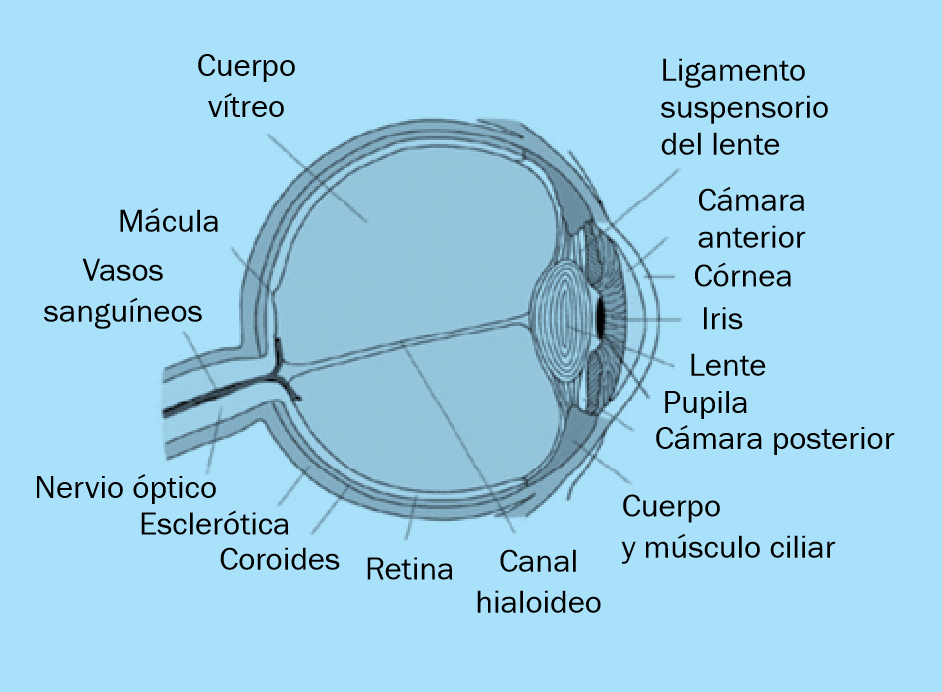
\includegraphics[width=0.45\textwidth]{imaxes/ojo1.png}
    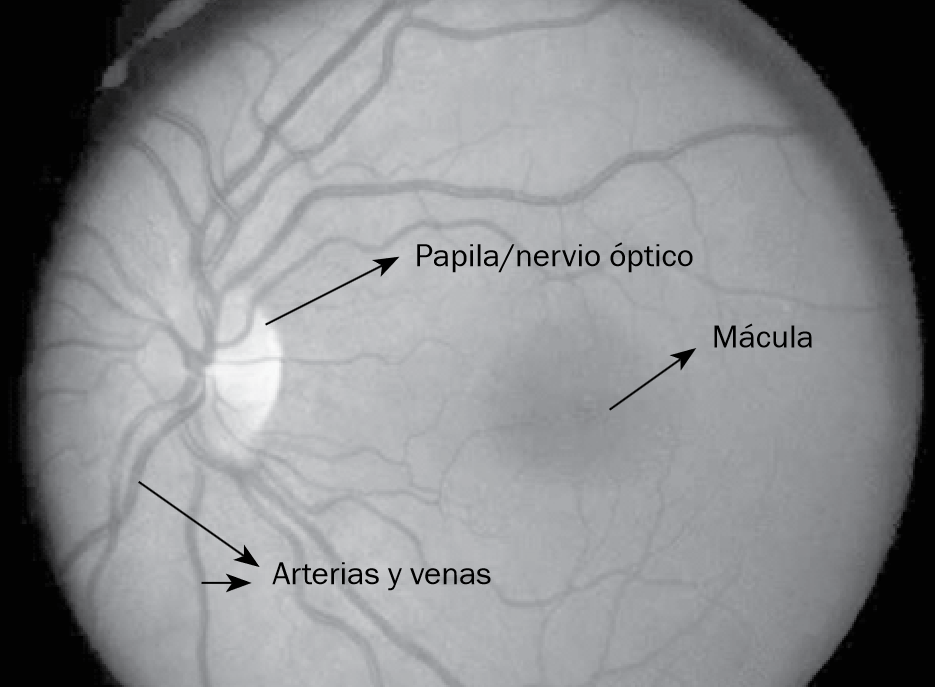
\includegraphics[width=0.45\textwidth]{imaxes/ojo2.png}
    \caption{Imágenes del ojo humano, extraídas de \cite{visionyojo}. A la izquierda, vista lateral del ojo anotada. A la derecha, retinografía del ojo anotada.}
    \label{fig:imaxes_ojo}
\end{figure}

\subsection{Imagen oftalmológica}
\label{subsec:Imaxe oftalmolóxica}
Existen diversas modalidades de imagen médica que permiten observar el ojo, cada una con diferentes propiedades y aplicaciones.
Entre ellas se incluyen la fotografía de fondo de ojo, la tomografía de coherencia óptica (OCT) y la angiografía con fluoresceína \cite{ilginis2014ophthalmic}.

Este trabajo se centra en la fotografía de fondo de ojo entre otras razones por su uso común en la práctica clínica.
Esto se debe en gran parte a su accesibilidad, requiriendo equipo más barato y menor entrenamiento comparada con las otras modalidades.
Además, es una técnica no invasiva y rápida de realizar, lo que la hace preferible en la mayoría de los casos \cite{retinimaging}.

Para realizarla se hace uso de una cámara especial denominada retinógrafo, y generalmente requiere de la previa dilatación de la pupila del paciente.
De esta forma se permite mayor entrada de luz en los ojos, lo que provoca una mejor visualización de la retina y mejora la calidad de la imagen.
Un especialista puede analizar la retinografía para detectar signos de enfermedades como la retinopatía diabética, la hipertensión o la degeneración macular \cite{retreggood}.

\section{Registro de imágenes}
\label{sec:Rexistro de imaxes}
El registro de imágenes es un proceso que consiste en, sobre dos o más imágenes, determinar la correspondencia espacial entre ellas
y alinearlas en un sistema de coordenadas común, con el objetivo de que las características de interés se encuentren en la misma posición.

El registro de imágenes tiene utilidad en muchos campos diferentes como la imagen satelital, geografía, robótica... pero el
campo de la imagen médica es de los más interesantes por su aplicación práctica y es el que se aborda en este trabajo \cite{goshtasby2017theory}.
Estas imágenes pueden variar a nivel temporal, espacial, de dimensión o de modalidad.

En el ámbito de la salud un registro adecuado puede emplearse para comparar imágenes de un mismo paciente tomadas en distintos momentos, en distintas modalidades o para comparar entre diferentes pacientes.
Esto permite la revisión del avance de una enfermedad a lo largo del tiempo, la fusión de imágenes de distintas modalidades o la detección de patrones comunes entre distintos individuos.
La fusión de imágenes permite interpretar mucho mejor la información disponible en ellas, y es de gran ayuda para guiar a los médicos en la toma de decisiones.
También es útil para corregir los movimientos involuntarios del paciente durante la adquisición de imágenes, como en el caso de la respiración en imágenes de pulmones, o para la intervención guiada por imagen (\gls{IGRT}) que no
podría funcionar sin la utilización adecuada de técnicas de registro de imágenes \cite{wang2022neuralrenderingstereo3d}.

Hasta recientemente, gran parte del trabajo de registro se hacía de forma manual por expertos con software como BigWarp \cite{bigwarp},
y dependía de las habilidades del profesional para detectar las características de interés y realizar el alineamiento.
Esto hacía que el proceso fuese lento y propenso a errores, además de poco práctico para grandes volúmenes de imágenes.

En la figura \ref{fig:retin_reg} se muestra un ejemplo de registro de imágenes de retina, donde se puede observar cómo las imágenes son alineadas para que las estructuras anatómicas coincidan.

\begin{figure}[tbp]
    \centering
    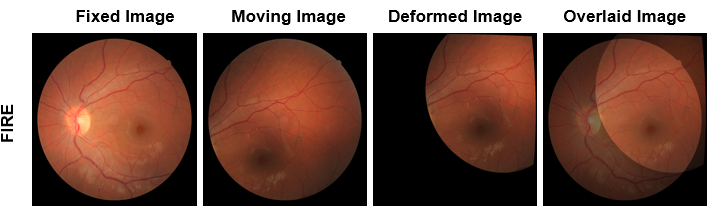
\includegraphics[width=0.8\textwidth]{imaxes/retin-reg.png}
    \caption{Ejemplo de registro de imágenes de retina \cite{sivaraman2024retinaregnetzeroshotapproachretinal}}
    \label{fig:retin_reg}
\end{figure}

\subsection{Categorías de registro}\label{subsec:Categorías de registro}

El registro de imágenes puede ser clasificado en distintas categorías según sus características.

\begin{itemize}
    \item \textbf{Según el número de imágenes:}
    \begin{itemize}
        \item \textit{Par a par:} El registro se realiza entre dos imágenes, una fija y una móvil.
        \item \textit{Múltiple:} Se registran varias imágenes simultáneamente, buscando una correspondencia global.
    \end{itemize}

    \item \textbf{Según la modalidad:}
    \begin{itemize}
        \item \textit{Intra-modalidad:} Las imágenes pertenecen a la misma modalidad (por ejemplo, dos retinografías).
        \item \textit{Inter-modalidad:} Las imágenes provienen de modalidades diferentes (por ejemplo, retinografía y OCT).
    \end{itemize}

    \item \textbf{Según el tipo de transformación:}
    \begin{itemize}
        \item \textit{Rígida:} Solo permite traslación y rotación, manteniendo las distancias y ángulos.
        \item \textit{Afín:} Además de traslación y rotación, permite escalado y cizallamiento.
        \item \textit{Deformable (no rígida):} Permite deformaciones locales complejas y no lineales.
        \item \textit{Difeomórfica:} Transformación no rígida que es continua, invertible y diferenciable en todo su dominio. Si no tiene esta característica, no se puede garantizar que la transformación sea reversible, por lo que son preferidas en muchos casos \cite{han2022diffeomorphicimageregistrationneural}.
    \end{itemize}

    \item \textbf{Según el grado de automatización:} \cite{deeplernreview3dreg}
    \begin{itemize}
        \item \textit{Manual:} El usuario selecciona puntos de control o ajusta parámetros.
        \item \textit{Automático:} El proceso se realiza sin intervención humana, mediante algoritmos.
        \item \textit{Semiautomático:} Combina intervención manual y automática.
    \end{itemize}

    \item \textbf{Según la naturaleza de la transformación:}
    \begin{itemize}
        \item \textit{Simétrico:} La transformación es consistente en ambas direcciones entre las imágenes.
        \item \textit{Asimétrico:} La transformación se calcula solo en un sentido. Cuando se trabaja con imágenes de forma asimétrica, la imagen de referencia se denomina imagen fija y la imagen que se quiere registrar imagen móvil.
    \end{itemize}

\end{itemize}

Las transformaciones lineales globales suelen representarse en matrices de transformación, donde cada elemento de la matriz representa un parámetro de la transformación.

En el caso de transformaciones más complejas, se utilizan campos de vectores de deformación (\gls{DFV}s), que permite representar deformaciones locales en la imagen, haciéndola mucho más flexible para representar transformaciones no lineales y detalladas.
Los DFVs suelen ser representados con una matriz de igual tamaño a la imagen, donde cada elemento representa un vector que indica la dirección y la magnitud de la deformación.

Este trabajo se ubica en el registro de imágenes par a par, intra-modalidad y con transformaciones deformables. Es un proceso totalmente automático que produce transformaciones asimétricas.

En la figura \ref{fig:dfv_visualization} se muestran dos formas de visualizar un DFV: mediante flechas que indican la dirección y magnitud de la deformación, y aplicando la deformación a una cuadrícula para ver cómo se distorsiona.

\begin{figure}[tbp]
    \centering
    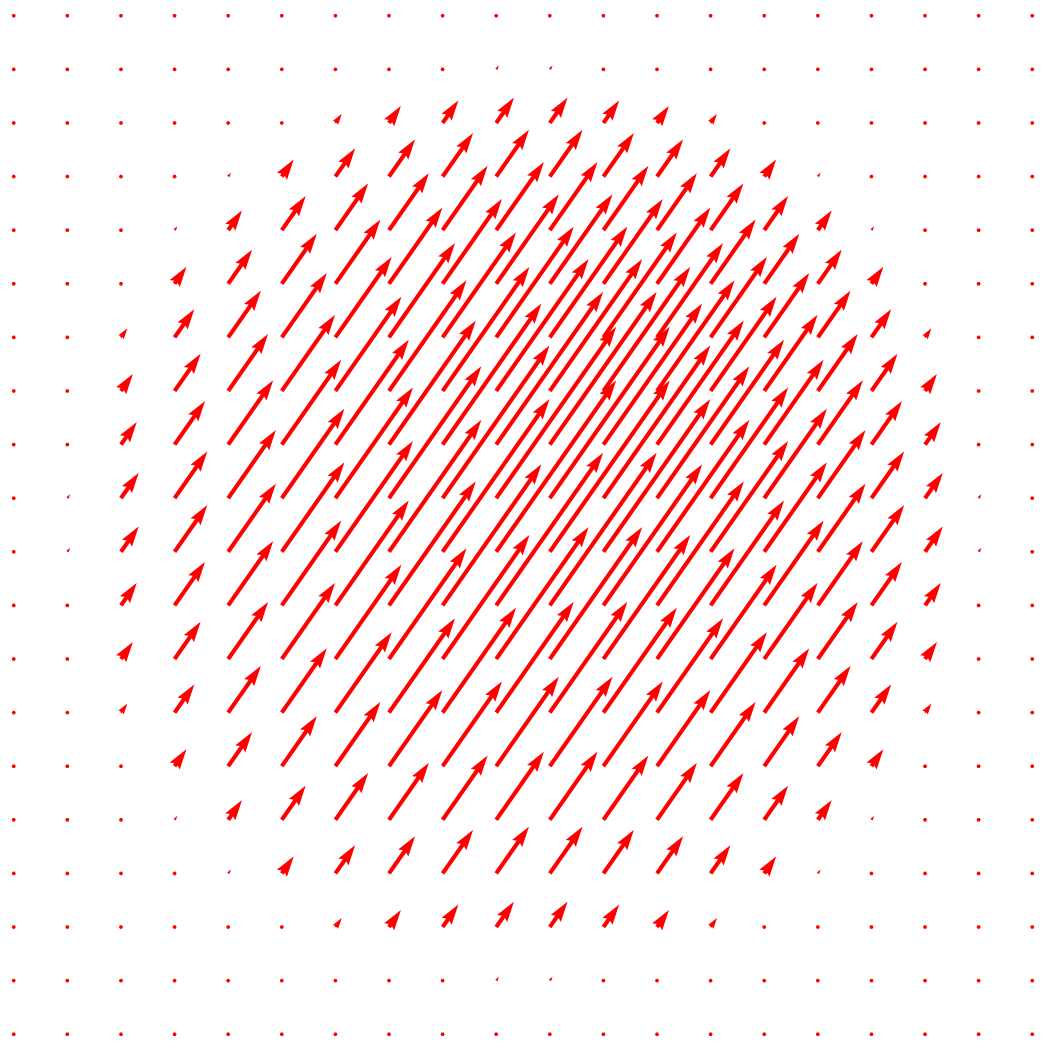
\includegraphics[width=0.45\textwidth]{imaxes/dfv_arrows.png}
    
\includegraphics[width=0.45\textwidth]{imaxes/dfv_grid.png}
    \caption{Visualización del campo de vectores de deformación (DFV). A la izquierda, representación mediante flechas. A la derecha, esta deformación aplicada a una cuadrícula.}
    \label{fig:dfv_visualization}
\end{figure}

\subsection{Estado del arte}
\label{subsec:Estado del arte}

El registro de imágenes médicas constituye un área de investigación fundamental que ha experimentado importantes avances en las últimas décadas. En este ámbito, la precisión y la robustez del registro cobran especial relevancia, ya que son empleados para el diagnóstico y seguimiento de enfermedades, así como para la planificación de tratamientos quirúrgicos.
En el campo de la oftalmología, los métodos que funcionan bien en varios dominios de imagen médica (cerebro, pulmones, etc) suelen requerir ajustes para funcionar en retinas, por lo que hay un estado del arte paralelo.

La evolución de los métodos de registro en retinografías refleja la transición desde enfoques puramente algorítmicos hacia metodologías híbridas, donde publicaciones recientes como HybridRetina \cite{liu2024progressiveretinalimageregistration} muestran cómo para alcanzar los mejores resultados es beneficioso combinar ambos enfoques, aprovechando la precisión de los métodos clásicos y la adaptabilidad de los métodos de aprendizaje automático.

\subsubsection{Métodos clásicos}\label{subsubsec:Métodos clásicos}

Los métodos clásicos de registro de imágenes médicas pueden clasificarse en dos categorías principales:
Aquellos basados en similitud de imagen (\gls{IBR}) y aquellos basados en características (\gls{FBR}).
También existen métodos híbridos que combinan ambos enfoques \cite{integrateintfeat}.
El resultado final puede ser los parámetros de la transformación o la imagen fusionada.

\paragraph{Métodos basados en similitud de imagen}
\label{par:Métodos basados en similitud de imagen}

El registro se realiza comparando los valores de intensidad de los píxeles o voxeles mediante una métrica de similitud entre la imagen fija y la imagen móvil.
Este enfoque tiende a requerir múltiples iteraciones para converger, en las cuales se calcula el grado de semejanza entre las imágenes y
se actualizan los parámetros de la transformación utilizando un mecanismo de optimización hasta que se cumplan los criterios de terminación.

Los métodos de registro tradicionales tienen tres componentes principales: la métrica de similitud, el optimizador y el modelo de transformación.

La figura \ref{fig:rexistro_iterativo} muestra un diagrama del proceso de registro iterativo.

\paragraph{Métodos basados en características}
\label{par:Métodos basados en características}

El registro se realiza identificando y emparejando características destacables entre las imágenes, como puntos, líneas o bordes.
Típicamente, estos métodos tienen 3 pasos principales:

\begin{itemize}
\item \textbf{Detección de puntos de interés:} Identificación de puntos o regiones destacables en las imágenes, como bordes, esquinas o texturas. Para esto pueden utilizarse algoritmos como SIFT \cite{sift}, SURF \cite{surf}, BRISK \cite{brisk} o FREAK \cite{freakkeypoint}.
\item \textbf{Descripción de características:} los puntos detectados son descritos y comparados entre imágenes usando descriptores.
\item \textbf{Estimación de la transformación:} una vez encontradas las correspondencias, se calcula la transformación que alinea las imágenes con algoritmos de emparejamiento como FLANN \cite{flann} o RANSAC \cite{ransac}.
\end{itemize}

Algunos de los métodos tradicionalmente más utilizados en este campo son \gls{GDB-ICP} \cite{GDB-ICP} y Harris-PIIFD \cite{piifd}. Este último utiliza el algoritmo Harris \cite{Harris1988ACC} para la detección de puntos de interés, los describe con \gls{PIIFD}, y se emparejan usando \gls{BBF} \cite{BBF}.
Finalmente, se refinan las coincidencias y se elige la transformación (rígida, afín o polinomial) según el número de pares de puntos válidos. Sobre esta base se han propuesto varias mejoras para adaptarlo al registro multimodal de retinas como UR-SIFT \cite{ur-sift} o \gls{GMM} \cite{GMM}.

Una ventaja de este enfoque es la capacidad para registrar imágenes con grandes variaciones locales o modalidades diferentes, ya que no depende tanto de la semejanza global entre las imágenes.

Otros métodos clásicos relevantes en el campo de la imagen de ojo incluyen REMPE \cite{rempe}, que estima simultáneamente la pose de las cámaras y la forma del ojo. Hace uso de un modelo elipsoidal para el ojo y estima la posición de las cámaras con RANSAC, para luego refinarla con una variante de PSO \cite{pso}.

\begin{figure}[tbp]
\centering
\begin{tikzpicture}[node distance=2cm, scale=0.8, every node/.style={transform shape}]
% Nodes
\node (imageFixa) [process] {Imagen Fija};
\node (imageMobil) [process, right of=imageFixa, xshift=3cm] {Imagen Móvil};
\node (featureExtraction) [process, below of=imageFixa, yshift=-1cm] {Cálculo de medida de similitud};
\node (parameterUpdate) [process, below of=featureExtraction, yshift=-1cm] {Actualización de Parámetros};
\node (applyTransformation) [process, below of=parameterUpdate, yshift=-1cm] {Aplicar la Transformación};
\node (criteriaCheck) [decision, below of=applyTransformation, yshift=-1cm] {¿Criterios Cumplidos?};
\node (result) [process, below of=criteriaCheck, yshift=-1cm] {Resultado};
% Arrows
\draw [arrow] (imageFixa) -- (featureExtraction);
\draw [arrow] (imageMobil) -- (featureExtraction);
\draw [arrow] (featureExtraction) -- (parameterUpdate);
\draw [arrow] (parameterUpdate) -- (applyTransformation);
\draw [arrow] (applyTransformation) -- (criteriaCheck);
\draw [arrow] (criteriaCheck) -- node[anchor=west] {Sí} (result);
\draw [arrow] (criteriaCheck.east) -- ++(1,0) node[anchor=south, xshift=0.5cm] {No} |- (featureExtraction.east);
\end{tikzpicture}
\caption{Proceso de registro de imágenes iterativo}
\label{fig:rexistro_iterativo}
\end{figure}

También existen múltiples programas que hacen uso de estos métodos en herramientas para facilitar el registro de imágenes, como SimpleITK \cite{simpleitk}, Elastix \cite{elastix} o ANTs \cite{ants}.

\subsubsection{Métodos de aprendizaje profundo}\label{subsubsec:Métodos de aprendizaje profunda}

Con la llegada de los métodos de aprendizaje profundo a la imagen médica, comenzaron a emplearse redes neuronales para realizar el alineamiento de imágenes.
Existe un gran interés por los métodos basados en aprendizaje profundo, como se refleja en el creciente número de publicaciones en el campo. En la figura \ref{fig:method_comp} se muestra la evolución del número de publicaciones sobre registro de imágenes, diferenciando entre los métodos basados en aprendizaje profundo y los métodos tradicionales.

Los métodos de aprendizaje profundo pueden ser clasificados en dos tipos según si requieren de \glossary{DFV}s anotados o no en la etapa de entrenamiento:
supervisados (requieren anotaciones) y no supervisados (no requieren anotaciones) \cite{nie2024medicalimageregistrationapplication}.

Según el grado de supervisión utilizado en la etapa de entrenamiento, los métodos supervisados pueden dividirse en supervisados o débilmente supervisados.
El registro totalmente supervisado hace uso de DVFs de referencia para supervisar el proceso de aprendizaje, y el término de pérdida suele basarse en la discrepancia entre los DVFs de referencia y los DVFs predichos.

El registro débilmente supervisado puede utilizar otras etiquetas de referencia implícitas, no basadas en datos explícitos como los DFVs, sino que utilizan información indirecta para guiar el proceso de registro, como la similitud entre las imágenes o restricciones basadas en la forma o límites anatómicos de las estructuras.
Más de dos tipos de datos de referencia son frecuentemente utilizados para entrenar modelos de registro débilmente supervisados \cite{bharati2022deeplearningmedicalimage}.

Los métodos no supervisados tienen la ventaja de no requerir datos anotados, lo cual es una gran ventaja ya que uno de los mayores retos para las redes de imágenes médicas es la recolección de datos de calidad para el entrenamiento \cite{medicalimageanalysis}.
La creación de conjuntos de DFVs anotados es un proceso laborioso y costoso, que normalmente solo puede ser ejecutado por especialistas, por lo que los métodos de registro no supervisados son de gran interés.
De forma similar a los métodos iterativos, es común emplear una métrica de similitud entre las imágenes junto con un término de regularización para guiar el proceso de optimización evitando caer en transformación no realistas.

Los enfoques de aprendizaje profundo son útiles tanto en su capacidad de aprender la tarea de registro de manera end-to-end, como para sustituir módulos concretos del proceso tradicional.
En ese sentido, los métodos de aprendizaje profundo pueden ser categorizados según la tarea del proceso de registro que sustituyen.

\begin{figure}[tbp]
\centering
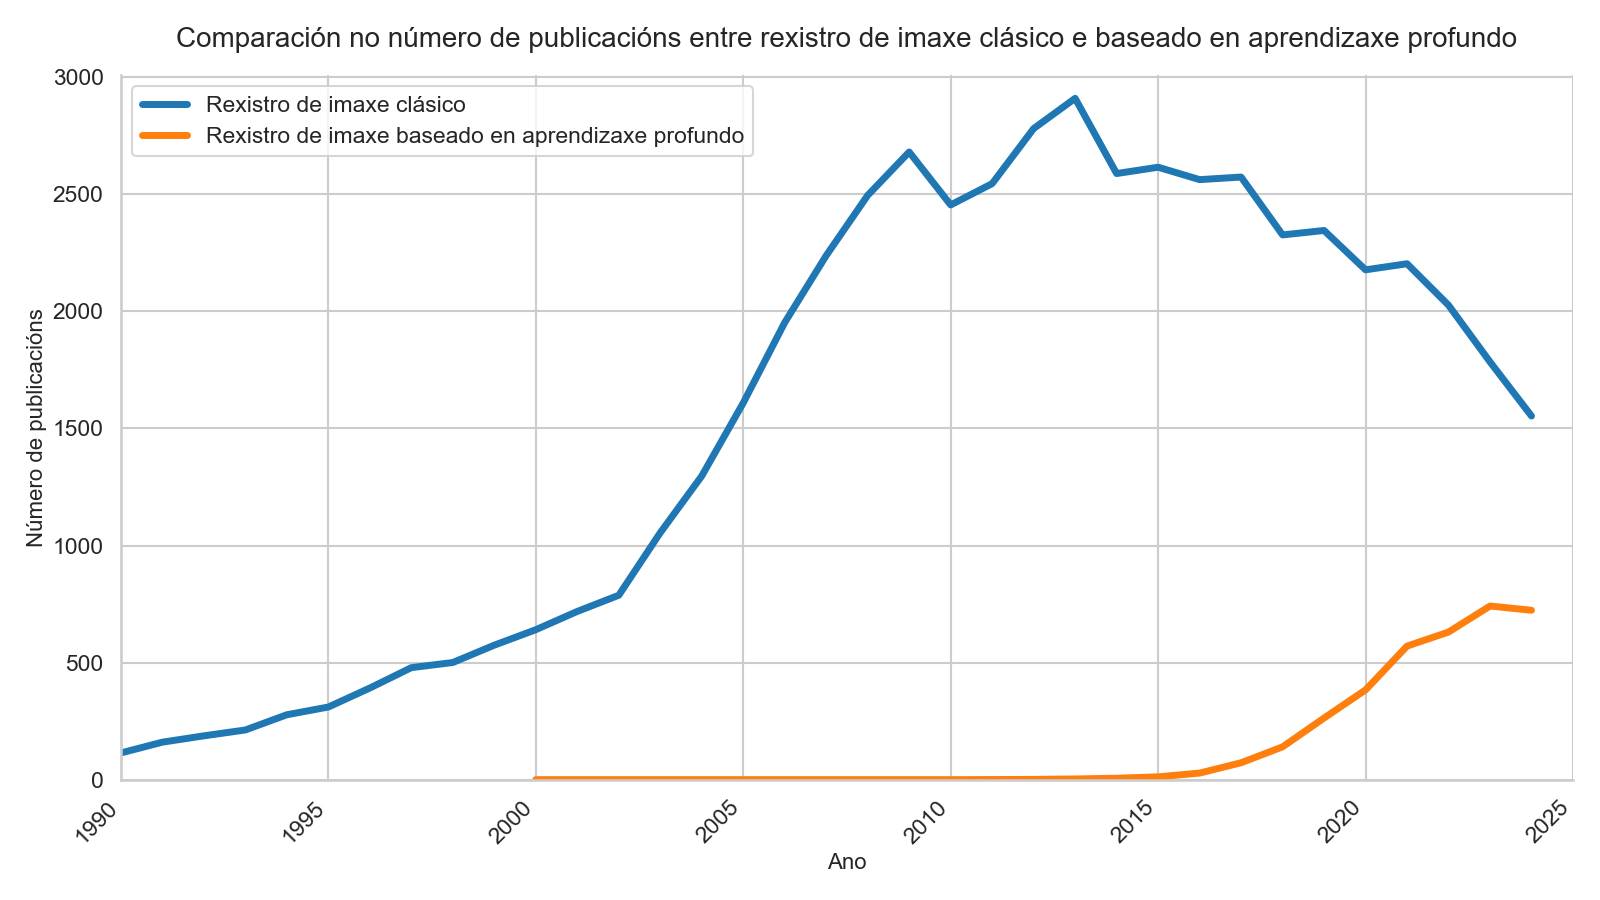
\includegraphics[width=0.8\textwidth]{imaxes/methods_comp.png}
\caption{Comparación de publicaciones a lo largo del tiempo relacionadas con el registro de imágenes. Datos extraídos de Scopus \cite{scopus}, realizando las consultas: "TITLE-ABS-KEY(image AND registration) AND NOT(deep AND learning)" y "TITLE-ABS-KEY(image AND registration) AND (deep AND learning)"}
\label{fig:method_comp}
\end{figure}

Los métodos de aprendizaje profundo pueden sustituir cualquiera de estos pasos que forman los métodos de registro clásicos de forma independiente o en combinación.

\paragraph{En registro basado en intensidad (IBR)}
\label{par:IBR_substitution}

\begin{itemize}
\item \textbf{Métrica de similitud:} Los métodos de aprendizaje profundo pueden aprender métricas de similitud más robustas que las tradicionales. Estas métricas aprendidas pueden ser más efectivas en imágenes multimodales o con artefactos.
Por ejemplo, Czolbe et al. \cite{semanticsimilarity} proponen dos métricas de similitud semánticas que aprende la semejanza entre imágenes comparando las características de alto nivel extraídas. Presentan una aproximación no supervisada que hace uso de autoencoders y otra semisupervisada que incorpora datos de segmentación.
\item \textbf{Optimizador:} Los métodos de aprendizaje profundo pueden sustituir el proceso de optimización iterativa tradicional por redes que aprenden a predecir directamente los parámetros de transformación óptimos. Una aproximación común es emplear estos conjuntos de datos para optimizar una CNN que, dadas dos imágenes nuevas y no vistas, predice el DFV correspondiente \cite{defregcnn}. Durante el proceso de entrenamiento, la red puede tener acceso a los DFVs con la deformación correcta, o se pueden obtener indirectamente a través de la optimización de una métrica de similitud de imágenes.
\item \textbf{Modelo de transformación:} Estos métodos aprenden representaciones implícitas de la transformación a través de redes neuronales, permitiendo modelar deformaciones más complejas que los modelos paramétricos tradicionales. Los métodos como IDIR \cite{wolterink2021implicit} encajan en esta categoría, utilizando campos neuronales implícitos para representar las transformaciones de registro.
\end{itemize}

\paragraph{En registro basado en características (FBR)}
\label{par:FBR_substitution}

\begin{itemize}
\item \textbf{Detectores de características:} Las redes neuronales pueden aprender a detectar puntos de interés más robustos y repetibles que los detectores clásicos como \glossary{SIFT}. SuperPoint \cite{superpoint} introduce un detector de características basado en redes neuronales que aprende a detectar puntos de interés y a describirlos simultáneamente.
\item \textbf{Descriptores de características:} Los descriptores aprendidos mediante redes neuronales pueden capturar información más discriminativa, mejorando la precisión del emparejamiento posterior. Estos métodos aprenden representaciones que son invariantes a transformaciones específicas del dominio.
\item \textbf{Emparejamiento:} Las redes neuronales pueden aprender a realizar el emparejamiento de características de forma robusta, especialmente en presencia de cambios de iluminación o perspectiva. SuperGlue \cite{superglue} es un ejemplo de modelo que aprende a emparejar puntos de interés detectados utilizando una arquitectura basada en atención para capturar las relaciones entre los puntos.
\end{itemize}

\paragraph{Métodos de regresión directa}
\label{par:direct_regression}

El aprendizaje profundo tiende a requerir de una gran cantidad de datos para ser entrenados, lo que puede ser una desventaja ya que en muchos casos no se disponen de bases de datos anotadas del tamaño necesario.

Los métodos de regresión directa aprenden a mapear directamente desde un par de imágenes hasta los parámetros de la transformación, sin necesidad de optimización iterativa ni extracción explícita de características.

También son denominados métodos de inferencia amortizada debido a la capacidad de realizar múltiples inferencias (registros) tras un único proceso de entrenamiento, en contraposición a los métodos tradicionales que requieren optimización individual para cada par de imágenes.
Estos enfoques son útiles por su eficiencia computacional en la fase de inferencia. Voxelmorph \cite{Balakrishnan_2019voxelmorph} es uno de los frameworks más utilizados en el registro de imágenes deformable, haciendo uso de modelos basados en \gls{CNN}s y que también permite incorporar información auxiliar (como segmentaciones) si está disponible, mejorando así la precisión del registro.

Métodos como UDIR-Net \cite{undefreg} o DIO \cite{Jena_2025} también implementan estas ideas.

\subsubsection{Estado del arte en el registro de retinografías}\label{subsubsec:Estado_da_arte_no_rexistro_de_retinografías}

El registro de retinografías presenta un conjunto de desafíos únicos que lo distinguen de otros dominios de la imagen médica.
Uno de los principales obstáculos son las deformaciones no rígidas. Estas deformaciones pueden originarse por la proyección de la superficie 3D curva de la retina en una imagen 2D o variaciones en la forma del ojo de cada paciente. Además, es frecuente encontrar pares de imágenes con áreas de solapamiento mínimas lo que dificulta la identificación de correspondencias para el alineamiento. A esto se suman las variaciones de iluminación, contraste y color entre imágenes capturadas en diferentes situaciones, así como los cambios anatómicos inducidos por patologías, que alteran las estructuras utilizadas para el registro.
Finalmente, la escasez de conjuntos de datos públicos, especialmente para condiciones o poblaciones específicas, supone una barrera importante para el desarrollo de modelos de aprendizaje supervisado.

La dificultad para obtener campos de deformación de referencia para el entrenamiento impulsó el desarrollo de marcos no supervisados. Estos modelos se entrenan optimizando una función de pérdida basada en la similitud de imagen entre la imagen móvil deformada y la imagen fija, junto con un término de regularización sobre la suavidad de la deformación.

Dentro de los métodos clásicos, los basados en características (FBR) siguen siendo referentes en cuanto a precisión. Entre ellos destacan VOTUS \cite{Votus}, que es especialmente robusto en imágenes de poco solapamiento y representa los árboles vasculares como grafos para encontrar la correspondencia entre ellos. REMPE \cite{rempe} es otro método ya mencionado anteriormente en esta categoría.

En el campo del aprendizaje profundo, RetinaRegNet \cite{sivaraman2024retinaregnetzeroshotapproachretinal} es un modelo reciente de tipo "zero-shot" que utiliza características extraídas de modelos de difusión para establecer correspondencias, alcanzando resultados de vanguardia.

ConKeD (Contrastive Keypoint Descriptors) y su evolución, ConKeD++, se centran en perfeccionar la creación de descriptores de puntos de interés, uno de los componentes más críticos de los métodos basados en características (FBR).
La principal ventaja es que obtiene resultados comparables a los de los métodos clásicos de vanguardia (como REMPE y VOTUS) pero con tiempos de ejecución mucho más rápidos.

La mayoría de estos algoritmos son evaluados y comparados utilizando el conjunto de datos de referencia FIRE \cite{FIRE}, permitiendo una cuantificación objetiva del rendimiento.

\section{Representaciones Neuronales Implícitas}
\label{sec:Representación Neuronais Implícitas}

La representación de conocimiento es uno de los problemas más importantes en el área de la computación, y las redes profundas son una de las herramientas más útiles, especialmente en el campo de la visión por computador.
Tradicionalmente se emplean representaciones discretas, donde el espacio de entrada es dividido en celdas y cada celda es asignada un valor (por ejemplo nubes de puntos, matrices de píxeles o vóxeles...).
Una de las principales desventajas de estas representaciones es que su complejidad se incrementa rápidamente con el número de dimensiones representadas, además del coste de memoria asociado.

Las representaciones neuronales implícitas son un paradigma innovador que permite modelar señales continuas mediante funciones parametrizadas por redes neuronales.
Codifican la información como una función continua, que mapea valores de entrada a los valores correspondientes de salida, en lugar de almacenar directamente valores de características o señales.

Representar la señal como una función continua permite solucionar los problemas asociados a la discretización y se obtienen otra serie de ventajas.

Las INR son mucho más eficientes debido a la compresión de la información que realizan de forma implícita. Al mismo tiempo, permite un nivel de detalle no limitado por la resolución de la imagen, sino por la capacidad de la red.
Además, las representaciones continuas son diferenciables, lo que permite el cálculo de gradientes y derivadas de forma analítica en lugar de tener que aproximarlos por diferencias finitas.
Esto también implica que las representaciones implícitas son independientes de la resolución, lo que permite la reconstrucción en cualquier escala espacial.

Típicamente se emplea un MLP como arquitectura para representar la función implícita. No obstante, el uso de la función de activación ReLU tiende a no obtener los mejores resultados, debido a que son incapaces de representar deformaciones locales sin afectar a su comportamiento global \cite{rahaman2019spectralbiasneuralnetworks},
por lo que mucha investigación se dirige a encontrar alternativas que mejoren la representación de la señal. \cite{essakine2024standimplicitneuralrepresentations}

Una de estas alternativas es SIREN \cite{sitzmann2020implicitneuralrepresentationsperiodic}, sobre la que profundizaremos más adelante.
Otras propuestas incluyen \cite{ramasinghe2022periodicityunifyingframeworkactivations} propone las funciones de activación gaussianas como alternativa a SIREN, y argumenta que pueden obtener mejores representaciones y más robustas.
\cite{saragadam2023wirewaveletimplicitneural} aporta una nueva función de activación basada en wavelets, que parece ser especialmente útil para la representación de imágenes.

Las representaciones implícitas pueden ser clasificadas en dos categorías: generalizables y sobreajustadas \cite{yu2024neuraltrajectorymodelimplicit}.
Las representaciones sobreajustadas se centran en reproducir con precisión una única señal, mientras que las representaciones generalizables pueden modelar varias en una misma red.

\subsection{Aplicaciones}
\label{subsec:Aplicacións}

Las INR son utilizadas en todo tipo de campos, desde generación de imágenes \cite{reddy2022multiimplicitneuralrepresentationfonts}, pasando por
reconstrucción de objetos \cite{mildenhall2020nerfrepresentingscenesneural} \cite{mescheder2019occupancynetworkslearning3d} o modelado de señales complejas \cite{wu2021iremhighresolutionmagneticresonance}.

Las representaciones implícitas están recibiendo cada vez más atención de la comunidad médica, y son especialmente útiles para las tareas de imagen inversa, que requieren la reconstrucción de representaciones correctas a partir de datos incompletos o ruidosos \cite{molaei2023implicitneuralrepresentationmedical}.
Métodos como NeRP, propusieron el uso de representaciones implícitas para la reconstrucción de imágenes de resonancia magnética a partir de datos incompletos, y obtuvieron resultados comparables a métodos tradicionales \cite{shen2023nerpimplicitneuralrepresentation}.

NeRF hace uso de representaciones implícitas para sintetizar nuevos puntos de vista en escenas 3D \cite{mildenhall2020nerfrepresentingscenesneural},
optimizando una función volumétrica continua que modela la densidad de volumen y la radiancia emitida en cada punto del espacio.
Utilizan un MLP, cuya entrada es una única coordenada continua 5D (localización espacial (x, y, z) y dirección de visión (θ, φ))
y cuya salida es la densidad de volumen y la radiancia emitida dependiente de la vista en esa localización espacial.
La única entrada necesaria para optimizar su representación es un conjunto de imágenes con poses de cámara conocidas.
Este trabajo demuestra que las representaciones implícitas están capacitadas para modelar escenas 3D complejas con alta fidelidad visual.

Las representaciones implícitas también tienen bastante potencial en el campo de planificación de trayectorias,
donde se hace uso de INRs para modelar entornos y planificar trayectorias para uno o varios agentes \cite{yu2024neuraltrajectorymodelimplicit}.
La principal ventaja de hacerlo de esta forma frente a la forma tradicional (algoritmos computacionalmente intensos, especialmente para multi-agentes) es la velocidad a la que encuentran soluciones (por debajo del milisegundo en GPUs).
La mayor desventaja es que no garantizan la convergencia a una solución óptima y sin colisiones, pero los autores demuestran que la calidad de las trayectorias generadas es adecuada para la mayoría de las aplicaciones \cite{trajectinr}.

En el ámbito médico, se utilizan este tipo de representaciones para garantizar la seguridad del paciente durante la cirugía teleoperada y optimizar la trayectoria del robot para evitar colisiones con el paciente, por ejemplo en la boca y garganta \cite{teleoperatdrob}.
Con este método, se evita la reconstrucción de mallas a partir de imágenes, que es un proceso costoso e imperfecto, y se modela mediante una INR a partir de los datos médicos disponibles.
Los comandos de movimiento de la mano del operador son tomados como entrada por el modelo, que después de un proceso de optimización, genera una secuencia de movimientos libre de colisiones que será enviada a la mano robótica.
También son utilizadas para crear reconstrucciones 3D de pulmones que mitigan las distorsiones causadas por el movimiento respiratorio \cite{velikova2024implicitneuralrepresentationsbreathingcompensated}.

Otro uso interesante de las representaciones neuronales implícitas es la compresión de imágenes. Algoritmos como COIN \cite{coin} representan los datos de entrada mediante redes neuronales implícitas (funciones que mapean coordenadas a valores RGB), logrando una compresión eficiente y una reducción significativa del tiempo de codificación en muchas modalidades.

\subsection{Registro basado en Representaciones Neuronales Implícitas}\label{subsec:Rexistro_baseado_en_INRs}

El registro de imágenes basado en Representaciones Neuronales Implícitas (INR) parametriza la transformación de deformación como una función continua, generalmente con un Perceptrón Multicapa (MLP), que mapea coordenadas espaciales a vectores de desplazamiento. A diferencia de las CNN, la red no procesa las intensidades de la imagen directamente, sino que se optimiza usando estas para calcular la pérdida. Una de las ventajas en este contexto es la capacidad de calcular gradientes analíticos exactos de la transformación, permitiendo una regularización más precisa que con aproximaciones de los métodos basados en rejillas.

Las funciones de activación periódicas (SIREN \cite{sitzmann2020implicitneuralrepresentationsperiodic}) permitieron superar el problema de los sesgos hacia transformaciones de baja frecuencia del MLP, y fueron utilizadas por IDIR alcanzando resultados de vanguardia \cite{wolterink2021implicit}.

Los principales inconvenientes son la lentitud en la inferencia (requiere optimización para cada par de imágenes) y la tendencia a generar pliegues espaciales (deformaciones no realistas). La investigación actual se centra en modelos híbridos para mitigar estos problemas.
Algunos de los enfoques más relevantes incluyen:
SINR (Spline-enhanced INR) combina INR con B-splines, donde la red predice los desplazamientos de una rejilla de control dispersa. Esto impone suavidad de forma intrínseca y facilita el registro multimodal \cite{SINR}.
INR ciclo-consistentes, que entrenan simultáneamente la transformación directa y la inversa, usando cada red como regularizador de la otra para mejorar la robustez.
Meta-aprendizaje: Aprende una inicialización de pesos óptima a partir de un gran conjunto de datos para acelerar drásticamente la convergencia en la inferencia \cite{learnedinit}.
INR condicionadas por geometría: Incorporan conocimiento anatómico previo para simplificar la complejidad de la deformación a aprender \cite{harten2023deformable}.
Sun et al. \cite{sun2024medicalimageregistrationneural} proponen un registro de imágenes que usa campos neuronales para modelar la transformación, utilizando también codificación posicional (que transforma las coordenadas espaciales en vectores de alta dimensión) lo que permite que la red aprenda con mayor facilidad las transformaciones de alta frecuencia.

El uso de Representaciones Neuronales Implícitas (INR) para el registro de imágenes ofrece una precisión notable al modelar la deformación como una función continua y analíticamente diferenciable. Este enfoque, ejemplificado por el éxito inicial de IDIR, permite una regularización más exacta que los métodos basados en rejillas. No obstante, su aplicación práctica se ve obstaculizada por la lentitud de la optimización por cada par de imágenes y el riesgo de producir deformaciones no realistas con pliegues espaciales. El estado del arte actual tiende a abordar estos retos mediante la hibridación.

\section{Trabajo propuesto}
\label{sec:Traballo proposto}

El trabajo propuesto se ubica dentro de los métodos de aprendizaje profundo, y más concretamente en el registro de imágenes basado en intensidad (IBR) utilizando representaciones neuronales implícitas (INRs).

Como mostramos en este capítulo, a pesar del potencial de las representaciones neuronales implícitas en diversos dominios médicos, su aplicación específica al registro de retinografías permanece inexplorada.

Esta falta de investigación es especialmente relevante dadas las potenciales ventajas que ofrecen las INRs, como la capacidad de modelar deformaciones complejas y su independencia de la resolución.

Basándose en el framework introducido por \cite{wolterink2021implicit}, se propone modificarlo para adaptarlo a la tarea de registro de retinografías. El objetivo es conseguir registros consistentemente precisos, especialmente en el dataset de FIRE que contiene imágenes reales de retina.

Esta adaptación representa una contribución novel al estado del arte en el registro de retinografías, explorando por primera vez el potencial de las representaciones neuronales implícitas en este dominio específico.
 \chapter{Metodología y planificación}
\label{chap:Metodoloxía e planificación}
\lettrine{E}{n} esta sección se explica la metodología de trabajo empleada para el desarrollo del proyecto, así como la planificación del mismo.
Además, se describen los recursos utilizados y se hace una estimación de los costes asociados al proyecto.

\section{Metodología del desarrollo}
\label{sec:Metodoloxía do desenvolvemento}

Al ser un proyecto de investigación, la metodología de trabajo más adecuada es una metodología iterativa e incremental, que permite adaptarse a los cambios que van surgiendo durante el desarrollo del proyecto.
Esta metodología permite obtener un artefacto funcional al final de cada iteración, lo que permite obtener retroalimentación constante.
Cada iteración comienza con un análisis de lo que se quiere conseguir, seguida de las fases de diseño y codificación, y termina con una fase de testeo del producto.

\section{Planificación del proyecto}
\label{sec:Planificación do proxecto}
El proyecto inicialmente se divide en las siguientes fases principales:

\begin{itemize}
    \item \textbf{Revisión del estado del arte:}
    \begin{itemize}
        \item Estudio del dominio biológico: características de las imágenes oftalmológicas, su importancia y aplicaciones.
        \item Análisis de trabajos relacionados con IDIR, representaciones implícitas y segmentación de imágenes oftalmológicas mediante redes neuronales.
    \end{itemize}
    Esta fase se estimó en aproximadamente 3 semanas de trabajo, dada la necesidad de familiarizarse con el contexto e identificar soluciones previas relevantes.

    \item \textbf{Análisis del trabajo base:}
    \begin{itemize}
        \item Estudio en profundidad del código original de IDIR.
        \item Replicación de los resultados originales para verificar el funcionamiento correcto.
    \end{itemize}
    El esfuerzo estimado para esta tarea fue de 2 semanas, considerando el análisis del código y la puesta en marcha del entorno.

    \item \textbf{Adaptación al nuevo dominio:}
    \begin{itemize}
        \item Modificación de la arquitectura para trabajar con imágenes 2D en lugar de 4D.
        \item Implementación de las adaptaciones necesarias para imágenes oftalmológicas.
    \end{itemize}
    Esta etapa se estima una duración de 5 semanas, debido a la complejidad de las modificaciones y pruebas necesarias.

    \item \textbf{Evaluación y experimentación:}
    \begin{itemize}
        \item Diseño de una metodología de evaluación específica para el nuevo dominio.
        \item Realización de múltiples experimentos para optimizar el rendimiento.
        \item Validación de la efectividad en imágenes oftalmológicas.
    \end{itemize}
    Se estima un esfuerzo de 8 semanas, repartidas entre el diseño experimental, ejecución y análisis de los resultados de los distintos experimentos.

    \item \textbf{Documentación:}
    \begin{itemize}
        \item Redacción de la memoria final del proyecto.
        \item Análisis y presentación de los resultados obtenidos.
    \end{itemize}
    Para la documentación se reservaron 2 semanas, incluyendo la redacción, revisión y preparación de los anexos. La memoria será redactada a lo largo de todo el proceso, pero en esta fase final se revisará y completará.
\end{itemize}

En total, se estima una duración de 20 semanas para el proyecto, repartidas entre las distintas fases.
En la figura \ref{fig:planificacion_proxecto} se muestra el diagrama de Gantt que resume la planificación del proyecto, indicando las fases principales y su duración estimada.

\begin{figure}[tbp]
    \centering
    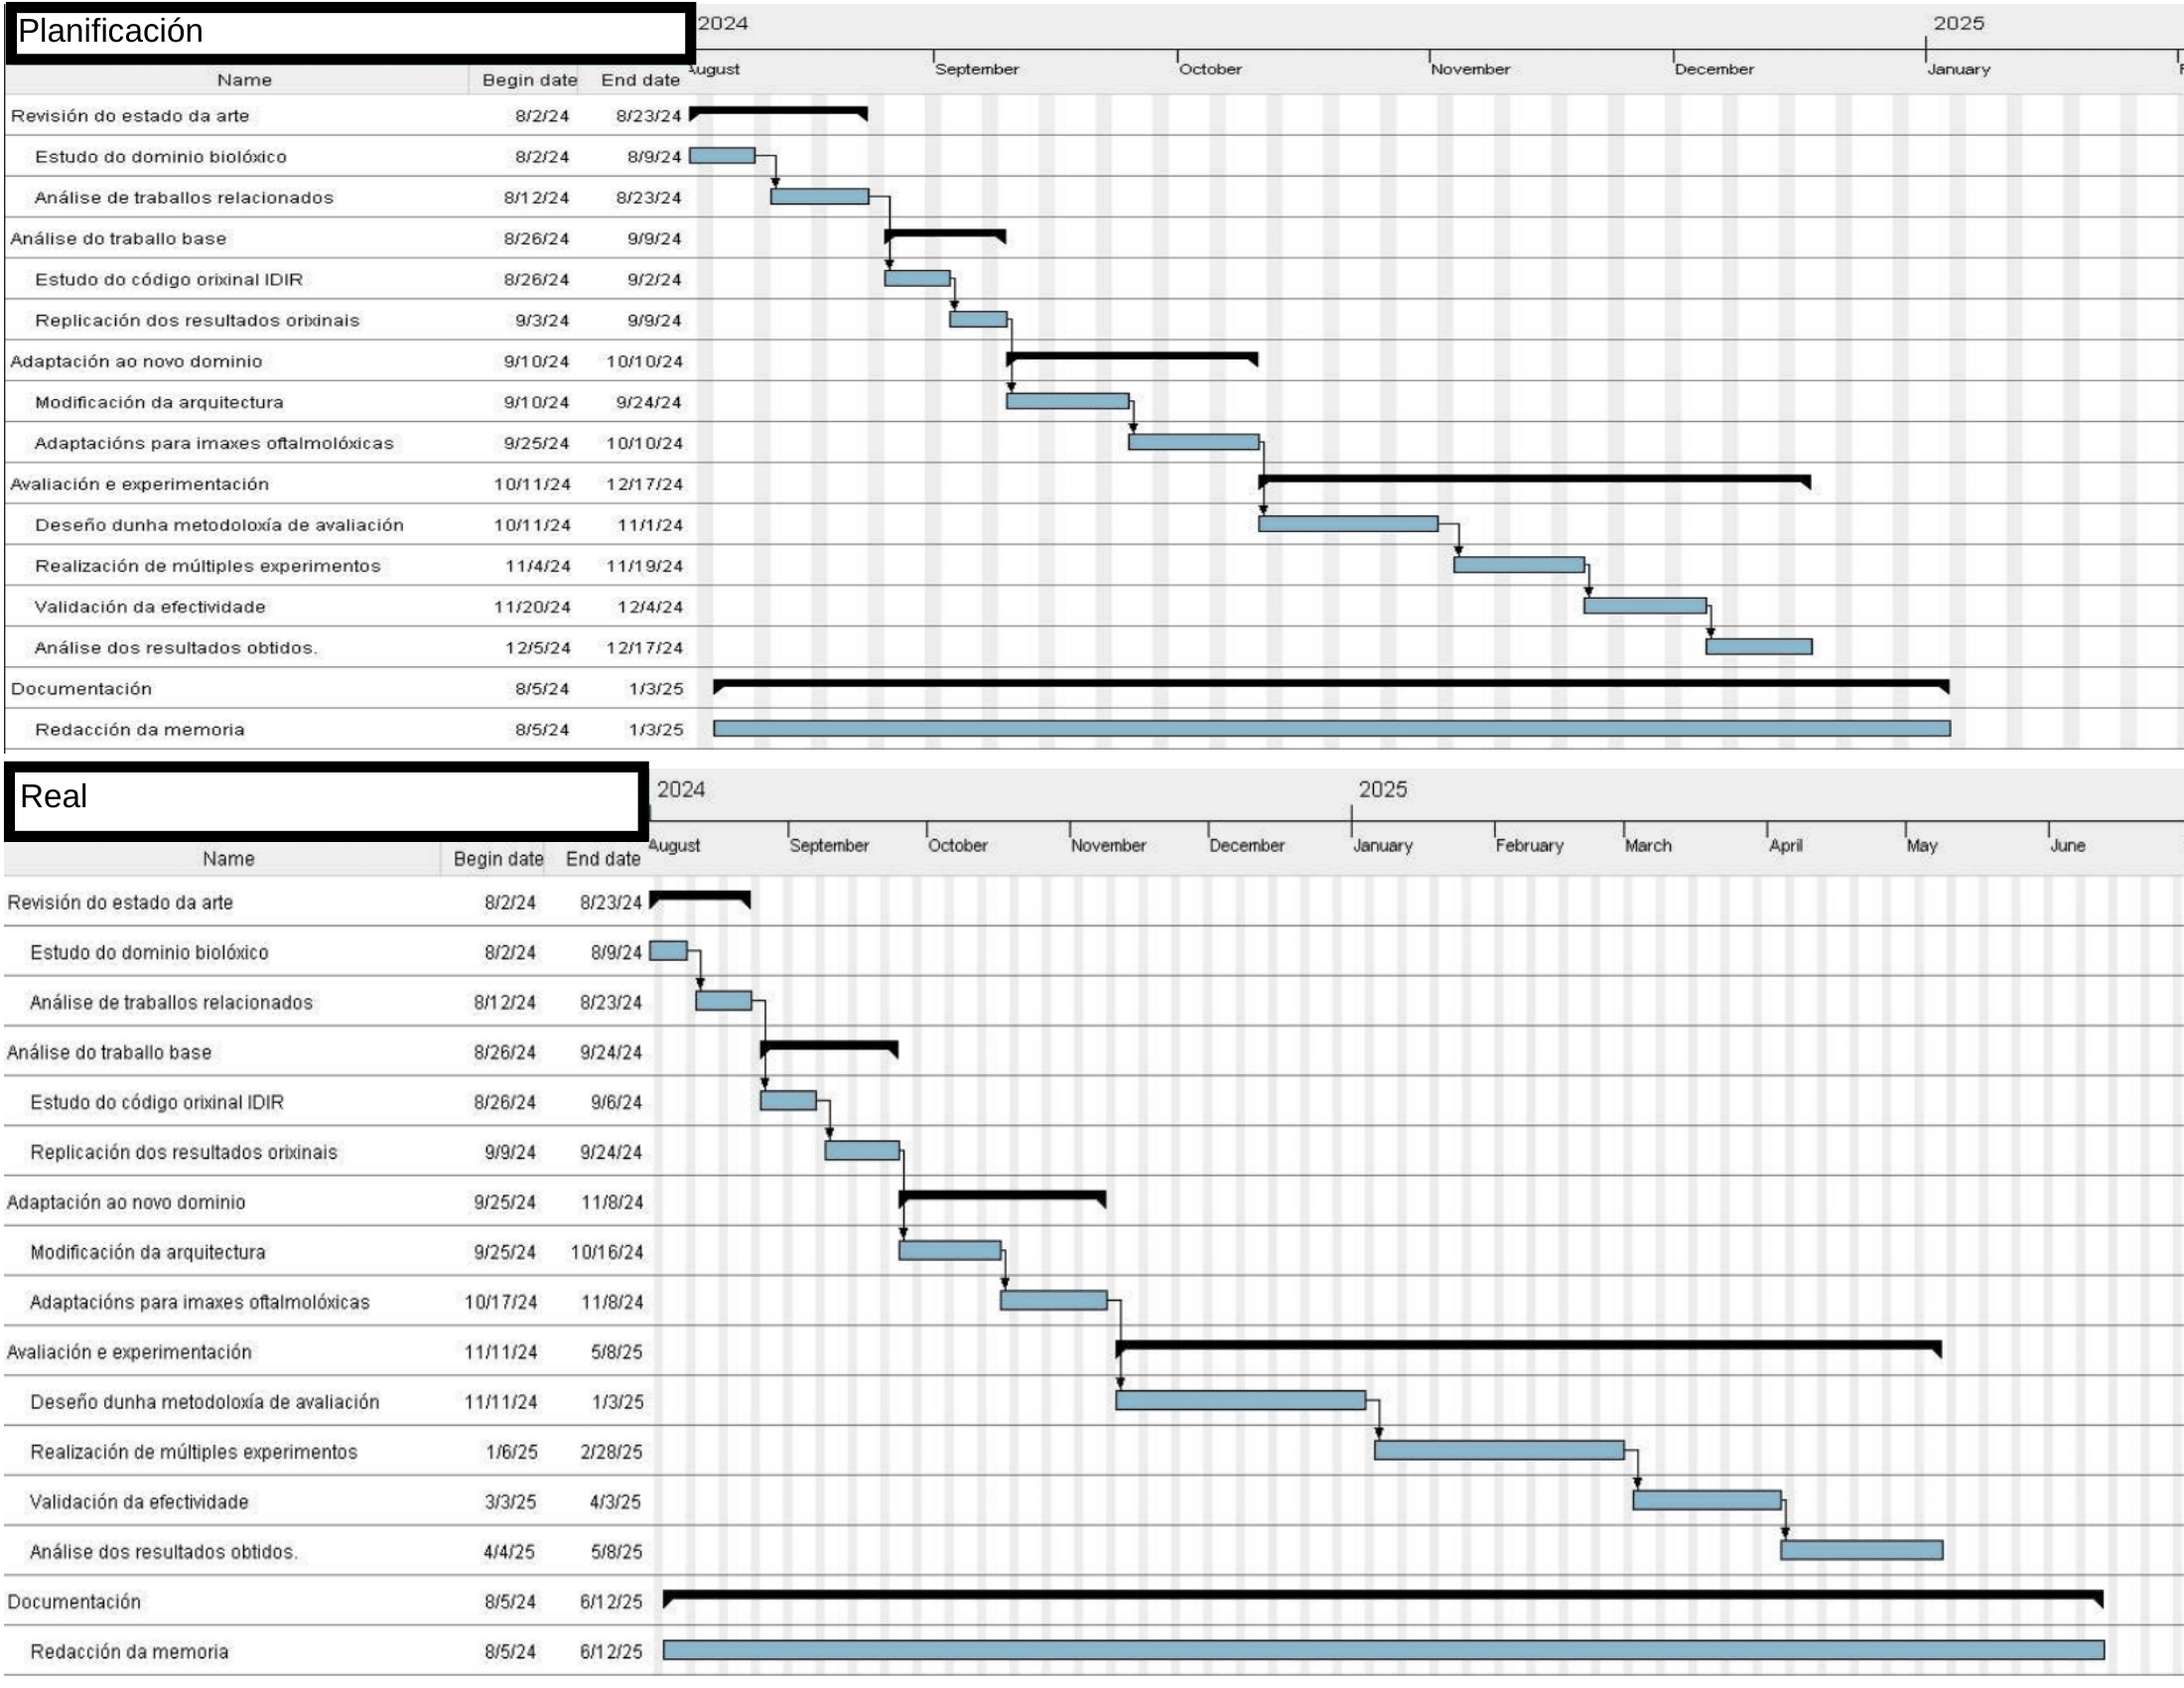
\includegraphics[height=1\textwidth, angle=90]{imaxes/gants-1.png}
    \caption{Diagramas de Gantt de la planificación del proyecto y duración real de cada fase}
    \label{fig:planificacion_proxecto}
\end{figure}

\section{Recursos utilizados}
\label{sec:Recursos utilizados}

\subsection{Software}
\label{subsec:Software}

Ya que parte del trabajo consiste en adaptar un trabajo previo,
se decidió emplear mucho del mismo software que el trabajo original para facilitar la implementación y reproducibilidad.
Lo más relevante es PyTorch, una librería de código abierto para Python que facilita la elaboración de redes neuronales. Se utilizaron las versiones de Python 3.12.3 y CUDA 12.2. También se emplean librerías de apoyo como NumPy (para trabajar con matrices), Matplotlib (visualización), OpenCV o scikit-learn (manejo de imágenes).

Otro software empleado incluye VSCode (IDE), Git (control de versiones) y LaTeX (redacción de memoria).

\subsection{Hardware}
\label{subsec:Hardware}

El proyecto fue desarrollado en un ordenador portátil conectado por ssh a un servidor con GPU.
Se utilizaron dos servidores diferentes, uno montado por mí\footnote{\url{https://blog.m19182.dev/writings/Building-my-Homelab}} y otro facilitado por el grupo de investigación VARPA (Visión Artificial y Reconocimiento de Patrones).

La gran parte de los experimentos fueron realizados en el primero, pero para poder ejecutar el proyecto con las imágenes en su resolución original fue necesario emplear el segundo
debido a las limitaciones de memoria de la GPU. En la tabla \ref{tab:comparativa_servidores} se muestra una comparativa entre los servidores utilizados, indicando las principales características de hardware de cada uno.

\begin{table}[tbp]
\centering
\begin{tabular}{|c|c|c|}
\hline
\textbf{Característica} & \textbf{Servidor Personal} & \textbf{Servidor VARPA} \\ \hline
Procesador & AMD Ryzen 9 5950X&  AMD Ryzen Threadripper 3960X \\ \hline
GPU & NVIDIA RTX 3090 & NVIDIA RTX A6000  \\ \hline
\end{tabular}
\caption{Comparativa entre los servidores utilizados}
\label{tab:comparativa_servidores}
\end{table}


\subsection{Conjuntos de datos}
\label{subsec:Conxuntos de datos}
Para el desarrollo del proyecto se emplearon dos conjuntos de datos diferentes:

\begin{itemize}
    \item \textbf{RFMID:} 3200 imágenes de fondo de ojo en color con resolución 1712x1712.
    \item \textbf{FIRE:} 134 pares de imágenes de retinas en color, con un tamaño de 2912×2912 píxeles
\end{itemize}

Estos son descritos en mayor detalle en la sección \ref{sec:Conxuntos de datos}.

\subsection{Estimación de costes}
\label{subsec:Estimación de custos}

Los costes del hardware son ignorados ya que ya estaba disponible antes de la realización del proyecto.

Los costes de los recursos humanos se calculan para un estudiante y dos tutores, resultando en un coste estimado de 20.680€, IVA incluido. La tabla \ref{tab:estimacion_custos} muestra la estimación de costes de los recursos humanos desglosados, considerando un estudiante a 20€/hora y tutores a 35€/hora.

\begin{table}[h]
\centering
\begin{tabular}{|c|c|c|c|}
\hline
\textbf{Recurso} & \textbf{Coste por hora} & \textbf{Horas estimadas} & \textbf{Coste total} \\ \hline
Estudiante & 20€ & 880h & 17.600€ \\ \hline
Tutor 1 & 35€ & 44h & 1.540€ \\ \hline
Tutor 2 & 35€ & 44h & 1.540€ \\ \hline
\end{tabular}
\caption{Estimación de costes de los recursos humanos (IVA incluido)}
\label{tab:estimacion_custos}
\end{table}

\section{Seguimiento de la planificación}
\label{sec:Seguimento da planificación}

La planificación del proyecto fue revisada periódicamente según las fases del proyecto, y para identificar desviaciones respecto al plan inicial.

A pesar de que en las fases iniciales del proyecto se respetó la planificación, la fase de adaptación al nuevo dominio y la fase de evaluación y experimentación sufrieron retrasos significativos.

La fase de adaptación al nuevo dominio requirió más tiempo del esperado debido a la complejidad de las modificaciones necesarias para adaptar el modelo a imágenes 2D, así como a la necesidad de realizar múltiples pruebas para garantizar el correcto funcionamiento del modelo adaptado. La fase de evaluación también se vio afectada, ya que requirió más tiempo del esperado para diseñar una metodología de evaluación adecuada. Finalmente, la fase de experimentación requirió más tiempo del previsto, en parte debido a los malos resultados obtenidos inicialmente, que obligaron a revisar en profundidad el código e implementar nuevas pruebas para asegurar la correcta implementación.
En total, esto conllevó un retraso de aproximadamente 18 semanas respecto a la planificación inicial.

La fase final de análisis de resultados y redacción de la memoria también se vio afectada, aunque en menor medida, lo que conllevó un retraso adicional de 2 semanas, resultando en una duración total del proyecto de 40 semanas, frente a las 20 semanas inicialmente previstas.

En la figura \ref{fig:planificacion_proxecto} se muestra el diagrama de Gantt actualizado, que refleja la duración real de cada fase del proyecto.

\subsection{Estimación de coste real}
\label{subsec:Estimación de custo real}

La estimación de coste del proyecto fue de 20.680€, como se indicó en la sección \ref{subsec:Estimación de custos}. No obstante, debido a los retrasos en el desarrollo del proyecto, el coste real aumentó de forma proporcional al tiempo extra empleado.

Dado que el proyecto se extendió durante 20 semanas más de lo previsto (el doble de la planificación inicial), el coste real estimado asciende a 41.360€ (IVA incluido).
 \chapter{Trabajo Realizado}
\label{chap:Traballo Realizado}

\lettrine{E}{n} este capítulo se presenta el trabajo realizado para adaptar el framework IDIR al registro de imágenes de retina en 2D. Se comienza con una vista general del proceso y una descripción detallada del método IDIR original, seguido de la explicación de las modificaciones realizadas para adaptar el sistema a las características específicas de las imágenes de fondo de ojo. Posteriormente, se describen los conjuntos de datos empleados, el diseño experimental desarrollado y los métodos de evaluación utilizados para validar los resultados.

\section{Vista General}
\label{sec:VistaXeral}

El trabajo realizado se centró en la adaptación del framework IDIR, originalmente diseñado para 4D-CT torácicas, al problema específico del registro de imágenes de fondo de ojo en 2D. Esta tarea requirió modificar la arquitectura de la red neuronal para operar en dos dimensiones, reformular los términos de regularización y adaptar los procesos de entrenamiento y evaluación para el nuevo dominio.
Para optimizar el modelo, se diseñó un proceso de experimentación sistemático y se desarrollaron metodologías de entrenamiento específicas. Entre ellas destacan la creación de estrategias de muestreo que priorizan regiones de interés anatómico y técnicas como el ajuste dinámico de hiperparámetros para refinar la convergencia del modelo.

Finalmente, para validar los resultados, se construyó un marco de evaluación que fue aplicado sobre los datasets FIRE (que contiene pares de imágenes reales con diferentes grados de superposición y variaciones anatómicas) y RFMiD (transformaciones lineales generadas), lo que permite juzgar distintas características de la red. La evaluación combinó métricas cuantitativas objetivas y el análisis cualitativo visual para garantizar la calidad y el realismo de las deformaciones obtenidas.

\section{IDIR}
\label{sec:IDIR}

IDIR (Implicit Deformable Image Registration) es un método de alineamiento de imágenes basado en redes neuronales.
Su principal diferencia frente a una red convolucional tradicional es que,

Lo que se propone es optimizar directamente el DFV haciendo uso de una representación implícita, de forma que la deformación está representada en los propios pesos de un MLP \cite{wolterink2021implicit}.

Otros trabajos como NIR \cite{sun2024medicalimageregistrationneural} o NODEO \cite{nodeo} proponen métodos de registro similares que también hacen uso de representaciones implícitas de las deformaciones, aplicados a resonancias magnéticas del cerebro.

\subsection{Arquitectura}
\label{subsubsec:Arquitectura}

Se hace uso de un MLP de 3 capas, y determinaron experimentalmente que obtenían mejor resultado con 256 unidades por capa que 128.
Por cada época de entrenamiento (2500 en total), 10000 puntos son muestreados aleatoriamente del espacio de coordenadas dentro de la máscara.
El término de pérdida es la 'normalized cross-correlation' entre los valores de los píxeles muestreados en la imagen fija y los correspondientes de la imagen móvil.
Utilizan Adam de optimizador, con un learning rate de 0.0001.

\subsubsection{Función de activación}
\label{subsubsec:Función de activación}

Una elección estándar para la función de activación es \textbf{ReLU}:

\[
f(x) = \max(0, x) = \begin{cases} 
x & \text{si } x > 0 \\ 
0 & \text{si } x \leq 0 
\end{cases}
\]

No obstante, para redes de representación implícita como con la que estamos trabajando, esta tiene una serie de desventajas.

Las ReLUs tienen un sesgo hacia señales de baja frecuencia \cite{rahaman2019spectralbiasneuralnetworks},
lo que significa que el modelo puede tener dificultades para representar pequeñas deformaciones locales en el registro de imágenes.

\cite{ziyin2020neuralnetworksfaillearn} demostraron que la gran parte de las funciones de activación utilizadas en redes neuronales (ReLU, tanh, sigmoide y todas sus variantes)
son incapaces de extrapolar funciones periódicas sencillas debido a su tendencia a converger hacia comportamientos lineales cuando se extrapolan fuera del rango de entrenamiento.

Existen varias formas de superar este sesgo, como preprocesar las coordenadas de entrada con funciones de activación periódicas \cite{mildenhall2020nerfrepresentingscenesneural}
o sustituir la función de activación ReLU por una función de activación periódica \cite{sitzmann2020implicitneuralrepresentationsperiodic}.

En este trabajo escogemos la segunda opción, utilizando una función de activación periódica de tipo \textbf{SIREN}:

\[
f(x) = \sin(ax + b), \quad \text{con} \quad a, b \in \mathbb{R}
\]

Una ventaja añadida de las funciones de activación periódicas en las redes SIREN es que pueden ser diferenciadas varias veces,
lo que expande sustancialmente el conjunto de términos de regularización que se pueden emplear en la red, como veremos en la siguiente sección.

larger frequencies appear in the networks for weights with larger magnitudes.

Otros trabajos como \cite{mildenhall2020nerfrepresentingscenesneural} no utiliza una función de activación periódica, pero para la representación adecuada de zonas de alta frecuencia
utilizaron codificación posicional, que ya las incorpora de forma implícita en la red con buenos resultados.

Otra de las ventajas que tiene SIREN es que es una función suave o infinitamente diferenciable, es decir, que admite derivadas de cualquier orden.
Otros ejemplos de funciones de activación infinitamente diferenciables son:

Sigmoide:
\[
f(x) = \frac{1}{1 + e^{-x}}
\]
Tangente Hiperbólica:
\[
f(x) = \tanh(x) = \frac{e^x - e^{-x}}{e^x + e^{-x}}
\]

Softplus:
\[
f(x) = \ln(1 + e^x)
\]

\paragraph{Inicialización de pesos}

En \cite{sitzmann2020implicitneuralrepresentationsperiodic} propusieron una inicialización específica para las redes SIREN,
la cual consiste en inicializar la primera capa de modo que la función seno recorra múltiples períodos sobre el intervalo [−1,1][−1,1].
Esto se consigue multiplicando los pesos de la primera capa por un factor de escala ω0, sobre el cual recomiendan ω0=30.
La fórmula para la inicialización de los pesos de la primera capa es la siguiente:

\begin{figure}[tbp]
    \centering
    \[
    w_i \sim U\left[ -\frac{1}{n}, \frac{1}{n} \right]
    \]

\caption{Inicialización primera capa}
\end{figure}

donde n es el número de neuronas de entrada (el tamaño de la capa anterior).

Las siguientes capas se inicializan de la siguiente forma:
\begin{figure}[tbp]
    \centering
    \[
    w_i \sim U\left[ -\frac{\sqrt{\frac{6}{n}}}{w}, \frac{\sqrt{\frac{6}{n}}}{w} \right]
    \]
    \caption{Inicialización siguientes capas}
\end{figure}

De esta forma se asegura que la entrada a cada activación sinusoidal está distribuida normalmente con una desviación estándar de 1,
lo que debería mejorar la estabilidad y convergencia durante el entrenamiento de la red.
Una consecuencia de esto es que, ya que los propios pesos de la red representan la deformación, inicialmente la red comienza con una deformación muy similar en todos los casos, que el entrenamiento deberá corregir.

En \cite{sireninit} implementan una versión simplificada de SIREN para facilitar el estudio de estas,
y proponen mejoras en el proceso de inicialización. Una de ellas es utilizar la distribución Kaiming (He) en lugar de la uniforme.
También proponen un método para escoger un valor de w apropiado según el problema a resolver.

\subsubsection{Términos de Pérdida}\label{subsubsec:Termos de Perda}

El término de pérdida es la función que se optimiza durante el entrenamiento, y es lo que guía la red hacia una solución óptima.
Esta cuantifica la discrepancia entre la salida de la red y el resultado deseado.

Para la tarea de registro de imágenes, se utilizan dos categorías principales de métricas para evaluar la alineación entre imágenes:
las métricas basadas en el error y las métricas basadas en la similitud. Las métricas basadas en el error (MSE, L1...) miden las diferencias píxel a píxel entre las imágenes,
siendo más sensibles a diferencias locales y proporcionando una medida absoluta.
Las métricas basadas en la similitud (NCC, SSIM...) tienen en cuenta patrones estructurales y relaciones estadísticas entre las imágenes, siendo más robustas frente a variaciones en la iluminación y pequeños desplazamientos.
\cite{simmetric}

Los principales términos de pérdida valorados para este trabajo son:

\begin{itemize}
    % Error-based metrics
    \item \textbf{MSE (Mean Squared Error)}:
    Error cuadrático promedio entre la imagen fija y la móvil. Es sensible a valores atípicos y ruido.
    \[
    \text{MSE} = \mathbb{E}[(Y - \hat{Y})^2] = \frac{1}{N} \sum_{i=1}^{N} (y_i - \hat{y}_i)^2
    \]
    donde \( y_i \) es el valor del píxel de la imagen fija, \( \hat{y}_i \) es el valor del píxel de la imagen móvil, y \( N \) es el número total de píxeles. \cite{Palubinskas02012017}

    Regularizador Hiperelástico en 2D   \item \textbf{L1 (Mean Absolute Error)}:
    Mide el error absoluto promedio. Menos sensible a valores atípicos que MSE.
    \[
    \text{L1} = \mathbb{E}[|Y - \hat{Y}|] = \frac{1}{N} \sum_{i=1}^{N} |y_i - \hat{y}_i|
    \]

    % Robust error metrics
    \item \textbf{Huber Loss}:
    Combina MSE y L1, siendo cuadrática para errores pequeños y lineal para errores grandes.
    \[
    \text{Huber}(y, \hat{y}) = \begin{cases}
    \frac{1}{2}(y - \hat{y})^2 & \text{si } |y - \hat{y}| \leq \delta \\
    \delta(|y - \hat{y}| - \frac{1}{2}\delta) & \text{en otro caso}
    \end{cases}
    \]
    donde \( \delta \) es un hiperparámetro que define el punto de transición entre los comportamientos cuadrático y lineal.

    \item \textbf{Smooth L1 Loss}:
    Similar a Huber Loss, pero con una transición suave entre las regiones cuadrática y lineal.
    \[
    \text{SmoothL1}(y, \hat{y}) = \begin{cases}
    \frac{1}{2}(y - \hat{y})^2 & \text{si } |y - \hat{y}| \leq 1 \\
    |y - \hat{y}| - \frac{1}{2} & \text{en otro caso}
    \end{cases}
    \]

    % Similarity-based metrics
    \item \textbf{NCC (Normalized Cross-Correlation)}:
    Evalúa la similitud entre las dos imágenes normalizando sus intensidades. Es invariante a cambios en la iluminación.
    \[
    \text{NCC} = \frac{\sum_{i=1}^{N} (y_i - \mu_y)(\hat{y}_i - \mu_{\hat{y}})}{\sqrt{\sum_{i=1}^{N} (y_i - \mu_y)^2 \sum_{i=1}^{N} (\hat{y}_i - \mu_{\hat{y}})^2}}
    \]
    donde \( \mu_y \) y \( \mu_{\hat{y}} \) son las medias de las imágenes fija y móvil, respectivamente.

    \item \textbf{SSIM (Structural Similarity Index)}:
    Evalúa la similitud estructural entre las dos imágenes, considerando luminancia, contraste y estructura.
    \[
    \text{SSIM}(y, \hat{y}) = \frac{(2\mu_y\mu_{\hat{y}} + C_1)(2\sigma_{y\hat{y}} + C_2)}{(\mu_y^2 + \mu_{\hat{y}}^2 + C_1)(\sigma_y^2 + \sigma_{\hat{y}}^2 + C_2)}
    \]
    donde \( \mu_y \), \( \mu_{\hat{y}} \) son las medias, \( \sigma_y \), \( \sigma_{\hat{y}} \) son las desviaciones estándar, \( \sigma_{y\hat{y}} \) es la covarianza, y \( C_1 \), \( C_2 \) son constantes para evitar divisiones entre cero. \cite{Palubinskas02012017}
\end{itemize}

Debido a la naturaleza de las imágenes de retina, donde pueden existir diferencias de iluminación y contraste entre las imágenes fija y móvil,
parece más apropiado emplear métricas basadas en la similitud como NCC o SSIM.

NCC se utilizó la implementación de https://github.com/BDdeVos/TorchIR/blob/main/torchir/metrics.py.

\subsubsection{Términos de regularización}\label{subsubsec:Termos de regularización}

Debido a que el registro de imágenes deformables es un problema mal formulado (ill-posed problem),
es común utilizar algún tipo de regularización sobre el DVF para evitar deformaciones poco realistas.
Los métodos de registro basados en redes neuronales convolucionales (CNN) representan los DVFs
como muestras en una cuadrícula de vóxeles, y por lo tanto, solo se pueden aproximar gradientes espaciales
mediante esquemas de diferencias finitas (aproximar derivadas mediante cálculo numérico de diferencias entre valores adyacentes en la cuadrícula).
Este es un proceso computacionalmente muy costoso e ineficiente, además implica errores de discretización y pérdidas de precisión.

Haciendo uso de representaciones implícitas, todas las operaciones son diferenciables, y los gradientes pueden
ser computados fácilmente de forma analítica en lugar de tener que aproximarlos, haciendo uso de la librería de autodiferenciación de PyTorch.

Utilizando ReLU como función de activación, la red es diferenciable una vez, mientras que utilizando
una función de activación periódica (como SIREN), la red es diferenciable todas las veces que se precise.
De esta forma, podemos calcular cualquier número de términos de regularización e incluirlos en la optimización de la red.

Algunos ejemplos de términos de regularización que se pueden emplear son:
\begin{itemize}
    \item Jacobian regularizer: 
    El determinante Jacobiano de la transformación (det ∇Φ) en una localización x es un indicador de estiramiento o compresión local.
    Un determinante Jacobiano negativo o muy cercano a 0 indica que están ocurriendo pliegues y la transformación no será invertible.
    La matriz jacobiana es la matriz que contiene todas las derivadas parciales de la función de transformación (calculado mediante gradientes).
    El término de regularización del Jacobiano penaliza los valores del determinante Jacobiano que se desvían de 1,
    intentando preservar áreas locales y evitar estiramientos o pliegues extremos.

    \begin{figure}[tbp]
        \centering
        \[
        S^{jac}[\Phi] = \int_{\Omega} \left| 1 - \det \left( \nabla \Phi \right) \right| \, dx
        \]
        \caption{Regulizador Jacobiano}
    \end{figure}

    Ω representa el dominio o región del espacio sobre el cual está definida la transformación Φ.
    
    \item Hyperelastic regularizer
    También se pueden añadir restricciones al DVF con este término propuesto por \cite{HyperelasticRegularization}.
    Consiste en tres términos, un término de longitud, un término de área y un término de volumen con el objetivo de controlar variaciones en estos aspectos.
    El término de longitud penaliza la variación de la longitud de los vectores del DVF, siendo u la medida desplazamiento de un punto en el espacio.
    La matriz de cofactores de la matriz del Jacobiano de la transformación controla el área,
    La función de máximo asegura que solo las expansiones que sobrepasen cierto límite sean penalizadas
    El determinante de la matriz del Jacobiano controla el volumen,
    y ambas penalizan el crecimiento y la contracción por igual.
    αl, αa y αν son hiperparámetros que controlan la importancia de cada término.

    \begin{figure}[tbp]
        \centering
        \[
        S^{hyper}[\Phi] = \int_{\Omega} \left[ \frac{1}{2} \alpha_1 |\nabla u|^2 + \alpha_a \varphi_c (\text{cof} \nabla \Phi) + \alpha_\nu \psi(\det \nabla \Phi) \right] dx,
        \]
        \[
        \text{Funciones convexas:} \quad \varphi_c(C) = \sum_{i=1}^3 \max \left\{ \sum_{j=1}^3 C_{ji}^2 - 1, 0 \right\}^2 \quad \text{and} \quad \psi(v) = \frac{(v-1)^4}{v^2}.
        \]
        \caption{Regulizador Hiperelástico.}
    \end{figure}


    \item Bending energy penalty
    Se puede imponer la suavidad de la deformación empleando esta penalización propuesta en \cite{bendingenergy}, que
    requiere que las segundas derivadas del DVF sean pequeñas en todo el dominio, lo que evita deformaciones bruscas y discontinuas.
    Este término no puede ser utilizado en una red que utilice ReLU como función de activación, ya que la segunda derivada de una ReLU es siempre igual a 0.

    \begin{figure}[tbp]
        \centering
        \[
        S^{bending}[\Phi] = \frac{1}{8} \int_{-1}^{1} \int_{-1}^{1} \int_{-1}^{1} \left[ \left( \frac{\partial^2 \Phi}{\partial x^2} \right)^2 + \left( \frac{\partial^2 \Phi}{\partial y^2} \right)^2 + \left( \frac{\partial^2 \Phi}{\partial z^2} \right)^2 \right.
        \]
        \[
        \left. + 2 \left( \frac{\partial^2 \Phi}{\partial x \partial y} \right)^2 + 2 \left( \frac{\partial^2 \Phi}{\partial x \partial z} \right)^2 + 2 \left( \frac{\partial^2 \Phi}{\partial y \partial z} \right)^2 \right] dx\,dy\,dz
        \]
        \caption{Regulizador Bending Energy}
    \end{figure}
    
\end{itemize}

Para la implementación en este trabajo se modificaron todos estos términos para que funcionaran con transformaciones de dos dimensiones en lugar de tres,
sustituyendo el gradiente de 3 dimensiones en el Jacobiano por uno de dos, eliminando las derivadas parciales en z en bending energy y el término de volumen en el término hiperelástico.

\begin{itemize}
    \item Jacobian regularizer:\\
    \[
    S^{jac}[\Phi] = \int_{\Omega} \left| 1 - \det \left( \nabla \Phi \right) \right| \, dx \, dy
    \]
    \item Hyperelastic regularizer:\\
    \[
    S^{hyper}[\Phi] = \int_{\Omega} \left[ \frac{1}{2} \alpha_1 |\nabla u|^2 + \alpha_a \varphi_c (\text{cof} \nabla \Phi) \right] dx \, dy,
    \]
    \[
    \varphi_c(C) = \sum_{i=1}^2 \max \left\{ \sum_{j=1}^2 C_{ji}^2 - 1, 0 \right\}^2
    \]
    \item Bending energy penalty:\\
    \[
    S^{bending}[\Phi] = \frac{1}{8} \int_{-1}^{1} \int_{-1}^{1} \left[ \left( \frac{\partial^2 \Phi}{\partial x^2} \right)^2 + \left( \frac{\partial^2 \Phi}{\partial y^2} \right)^2 + 2 \left( \frac{\partial^2 \Phi}{\partial x \partial y} \right)^2 \right] dx \, dy
    \]
\end{itemize}

La regularización también tiene un impacto significativo en el tiempo de computación, ya que requiere múltiples pasadas de retropropagación por época para calcular los distintos términos de penalización.
Sin regularización solo se hace 1 pasada para calcular el gradiente del término de similitud de la imagen.
Con la regularización del Jacobiano, además del término de similitud, se calculan dos derivadas (una por dimensión) para obtener el Jacobiano, resultando en 3 pasadas por época.
Añadiendo la regularización hiperelástica (sin término de volumen), es necesario calcular una derivada adicional para el cofactor de la matriz Jacobiana, haciendo un total de 4 pasadas por época.
Finalmente, con la penalización de energía de flexión, se necesitan derivadas segundas, lo que implica 7 pasadas por época en total.
En el trabajo original de IDIR, llegaban a usar 13 pasadas debido a que trabajan en 3D.

Si los términos de regularización tienen demasiada influencia sobre el término de pérdida, la red hará transformaciones muy pequeñas para evitar ser penalizada, lo que resultará en una transformación insuficiente.
Por otro lado, si los términos son demasiado pequeños, la red hará transformaciones muy grandes, lo que resulta en una transformación irrealista y sobreajustada. Esto es especialmente evidente en el caso de la función de activación SIREN, que tiende a sobreajustarse fácilmente debido a su sesgo hacia señales de alta frecuencia.
La cantidad óptima de regularización depende de la pareja concreta de imágenes a alinear, por lo que intentaremos determinar cuál es la mejor para una muestra de imágenes.

Además, pese a que los diferentes términos de regularización valoran diferentes aspectos, cabe tener en cuenta que también hay superposición en algunas de las propiedades que valoran.
Por ejemplo, el regularizador hiperelástico puede considerarse un término más general que incluye indirectamente penalizaciones del Jacobiano (ambos penalizan los "pliegues") y de suavidad de las transformaciones (como hace el bending pero en menor grado).

\subsubsection{Learning rate y tamaño de lote}
\label{subsubsec:Learning rate e tamaño de lote}

El learning rate es un parámetro del optimizador (Adam en este caso) que regula el tamaño de los ajustes efectuados a los parámetros del modelo durante cada iteración de actualización.
Determina la magnitud del cambio aplicado para minimizar la función de pérdida, afectando tanto a la velocidad de convergencia como a la estabilidad del proceso de aprendizaje.
Un learning rate demasiado alto puede provocar que la red diverja, mientras que un learning rate demasiado bajo puede resultar en convergencia lenta o quedar atrapado en mínimos locales.

Debido a la naturaleza de la red, el tamaño de lote utilizado tiene una relación directa con el learning rate, por lo que intentaremos determinar la relación óptima entre ambos.

Una de las heurísticas más comunes para relacionar el learning rate y el tamaño de lote es la regla de escalado lineal \cite{goyal2018accuratelargeminibatchsgd}.
La regla indica que el learning rate óptimo debe escalarse linealmente con la cantidad de muestras por lote.

Una forma de explicar esto es, ya que con tamaños de lote más grandes tenemos una mejor aproximación del gradiente real, es posible utilizar un learning rate mayor sin que la red diverja. \cite{kexuefm}

El tamaño de lote en esta red representa el número de coordenadas muestreadas aleatoriamente del espacio de coordenadas dentro de la máscara.

\subsection{Método}\label{subsubsec:Método}

Siendo el objetivo encontrar una transformación espacial óptima entre la imagen móvil y la imagen fija,
es necesario obtener la función de deformación Φ(x) = u(x) + x que mapea cada coordenada x en la imagen móvil a una coordenada en la imagen fija,
de forma que la coordenada x en la imagen fija corresponda anatómicamente a la coordenada Φ(x) en la imagen móvil.
Este problema puede ser formulado como un problema de optimización donde $L_{data}$ es una métrica de similitud entre las imágenes fija ($F$) y móvil ($M$), $L_{reg}$ es un término de regularización en la transformación Φ, y α es un término de ponderación.
\begin{equation}
    \hat{\Phi} = \operatorname*{Arg\,min}_{\Phi} L_{data}(M \circ \Phi, F) + \alpha L_{reg}(\Phi)
\end{equation}

La principal innovación que introduce IDIR\cite{wolterink2021implicit} es que la transformación Φ está implícitamente representada en la red neuronal.

Comparado con una CNN tradicional, esta red no recibe valores de intensidad de píxel como entrada,
sino que recibe coordenadas espaciales (continuas) y devuelve una nueva coordenada.
Ya que los pesos de la red definen la transformación, estos pueden ser optimizados directamente
haciendo uso de una métrica de similitud como función de pérdida.

Parametrizar la función de deformación como una \glossary{INR} dentro de un \glossary{MLP} tiene varias ventajas para el registro de imágenes.
En primer lugar, la representación de la transformación es continua y por lo tanto independiente de la resolución de la imagen,
gracias a ello el mismo modelo puede ser empleado para imágenes de cualquier tamaño, al contrario de una CNN tradicional
que tiene que ser adaptada para cada resolución.

Segundo, hacerlo de esta forma permite aprovechar las capacidades de librerías como PyTorch para calcular los gradientes de la transformación respecto a las coordenadas.
Esto permite obtener gradientes más precisos que las aproximaciones por diferencias finitas
y permite aprovechar una gran cantidad de literatura sobre regularización eficientes en imágenes médicas.

Tercero, se puede modificar la función de activación empleada en la red para ajustarla a las necesidades particulares de la tarea de registro de imágenes.

El \gls{NTK} describe cómo un modelo de red neuronal responde a cambios en sus parámetros durante el entrenamiento,
y dependiendo de la función de activación empleada, el NTK varía y la red puede ser más o menos sensible a ciertas deformaciones.

Finalmente, se entrenará una nueva red por cada pareja de imágenes, siendo esta una red bastante pequeña en comparación y prescindiendo de la necesidad de grandes conjuntos de datos para su entrenamiento.

\subsection{Replicación de resultados}
\label{subsec:Replicación de resultados}

Se replicaron los resultados obtenidos por Wolterink et al. \cite{wolterink2021implicit} que se muestran en la tabla \ref{tab:comparison}.

\begin{table}[ht]
    \centering
    \caption{Replicación de los resultados de IDIR}
    \begin{tabular}{c|c}
        Scan & {IDIR / Replicación} \\
        1  & 0.76 (0.94) / 0.79 (0.92) \\
        2  & 0.76 (0.94) / 0.71 (0.89) \\
        3  & 0.94 (1.02) / 0.95 (1.01) \\
        4  & 1.32 (1.27) / 1.32 (1.22) \\
        5  & 1.23 (1.47) / 1.23 (1.46) \\
        6  & 1.09 (1.03) / 1.15 (1.04) \\
        7  & 1.12 (1.00) / 1.11 (0.99) \\
        8  & 1.21 (1.29) / 1.20 (1.28) \\
        9  & 1.22 (0.95) / 1.16 (0.99) \\
        10 & 1.01 (1.05) / 1.09 (1.05) \\
        Promedio & 1.07 / 1.07 (1.08) \\
    \end{tabular}
    \label{tab:comparison}
\end{table}

\section{Adaptación a 2D}
\label{sec:Adaptación a 2D}

Para adaptar el modelo IDIR a 2D, es necesario modificar la arquitectura de la red para que funcione con imágenes bidimensionales.
La arquitectura original de IDIR tiene una entrada de 3 dimensiones (x, y, z) y una salida de 3 dimensiones (dx, dy, dz),
mientras que nuestra red tiene una entrada de 2 dimensiones (x, y) y una salida de 2 dimensiones (dx, dy).

Se modificaron las capas de entrada y salida de la red para que acepten coordenadas bidimensionales (originalmente [3, 256, 256, 256, 3], ahora [2, 256, 256, 256, 2]).

Fue necesario modificar las funciones de interpolación, que antes interpolaban valores tridimensionales y ahora interpolan valores bidimensionales.

También se adaptaron los términos de regularización para que funcionen con coordenadas bidimensionales, como se detalla en la sección \ref{subsubsec:Termos de regularización}.

Finalmente, el proceso de evaluación tuvo que implementarse desde 0 para adaptarse al nuevo formato de imágenes y datos de referencia.

\subsection{Proceso de Registro}
\label{subsec:Proceso de Registro}

El registro de cada par de imágenes (fija y móvil) se trata como un problema de optimización independiente. Para cada par, se entrena una nueva red neuronal desde cero cuyo único objetivo es aprender la deformación específica que alinea esas dos imágenes.

Primeramente, se crea una instancia del MLP con la arquitectura 2D y se definen los hiperparámetros como la función de activación, la métrica de pérdida y términos de regularización que se aplicarán. La inicialización de los pesos de la red es un paso de especial relevancia.

Una vez inicializada la red, se genera un tensor de coordenadas que contiene la localización (x, y) de todos los píxeles que se encuentran dentro de la máscara de la imagen fija. Este tensor representa el espacio de coordenadas completo sobre el que la red aprenderá la deformación.

A continuación, comienza el bucle de entrenamiento, que se repite durante un número predefinido de épocas. En cada iteración dentro de una época, se realiza el siguiente proceso:
\begin{itemize}
    \item \textbf{Muestreo de Coordenadas:} En lugar de procesar la imagen entera en cada paso, se selecciona un subconjunto de puntos del tensor de coordenadas igual al tamaño de lote. La estrategia de muestreo es un componente crítico que fue objeto de experimentación en este trabajo.

    \item \textbf{Predicción y Aplicación de la Transformación:} Las coordenadas (x, y) muestreadas se introducen en la red. El MLP actúa como una función de deformación implícita, devolviendo para cada coordenada de entrada un vector de desplazamiento (dx, dy).

    \item \textbf{Cálculo de la Pérdida (Loss):} Para cuantificar lo bien que la deformación alinea las imágenes, se comparan los valores de intensidad en los puntos seleccionados. Para cada coordenada original $(x,y)$ en la imagen fija, se obtiene el valor de intensidad correspondiente en la imagen móvil en la coordenada transformada $(x + dx, y + dy)$. Como esta última suele ser una posición no entera, se utiliza interpolación para estimar su valor de intensidad. La métrica de pérdida (NCC, SSIM, etc.) calcula la discrepancia entre el conjunto de intensidades de la imagen fija y el de las intensidades obtenidas de la imagen móvil transformada.

    \item \textbf{Retropropagación y Actualización:} Al valor de la pérdida de similitud se le suman los términos de penalización calculados a partir de los regularizadores. El valor de pérdida total resultante se utiliza para calcular los gradientes respecto a los pesos de la red mediante retropropagación. Finalmente, el optimizador (Adam) utiliza estos gradientes para actualizar los pesos del MLP, ajustándolos ligeramente en la dirección que minimiza la pérdida.
\end{itemize}

Este ciclo se repite hasta completar todas las épocas. Al final del entrenamiento, los pesos optimizados de la red encapsulan la función de deformación continua y específica para ese par de imágenes.

Es crucial subrayar que la tarea de registro de retinografías difiere sustancialmente de la de pulmones. Por este motivo, no es posible asumir que los hiperparámetros óptimos del trabajo original sean válidos para este nuevo dominio, lo que justifica la extensa experimentación realizada.

\section{Conjuntos de datos}
\label{sec:Conjuntos de datos}

\subsection{FIRE}
\label{subsec:FIRE}

Está compuesto por 134 pares de imágenes de retinas, con un tamaño de 2912 × 2912 píxeles y un \gls{FOV} de 45◦× 45◦.
Están clasificadas en 3 categorías según el grado de superposición y la presencia de diferencias anatómicas: \textit{S}, \textit{P} y \textit{A}. \cite{FIRE}

\begin{figure}[tbp]
    \centering
    \setlength{\tabcolsep}{8pt} % Adjust column spacing
    \begin{tabular}{|c|c|c|c|}
        \hline
        \textbf{Categoría} & \textbf{Nº de pares de imágenes} & \textbf{Superposición (\%)} & \textbf{Diferencias Visuales} \\
        \hline
        \textbf{\textit{\textsf{S}}} & 71 & > 75 & No \\
        \hline
        \textbf{\textit{\textsf{P}}} & 49 & < 75 & No \\
        \hline
        \textbf{\textit{\textsf{A}}} & 14 & > 75 & Sí \\
        \hline
    \end{tabular}
    \caption{Clasificación de los pares de imágenes en categorías.}
    \label{tab:categorias}
\end{figure}
\FloatBarrier

Incluye 10 puntos de referencia para cada imagen, que se utilizan para la evaluación del registro, así como una máscara por cada imagen que indica la localización de los píxeles con información de color.

\begin{figure}[tbp]
    \centering
    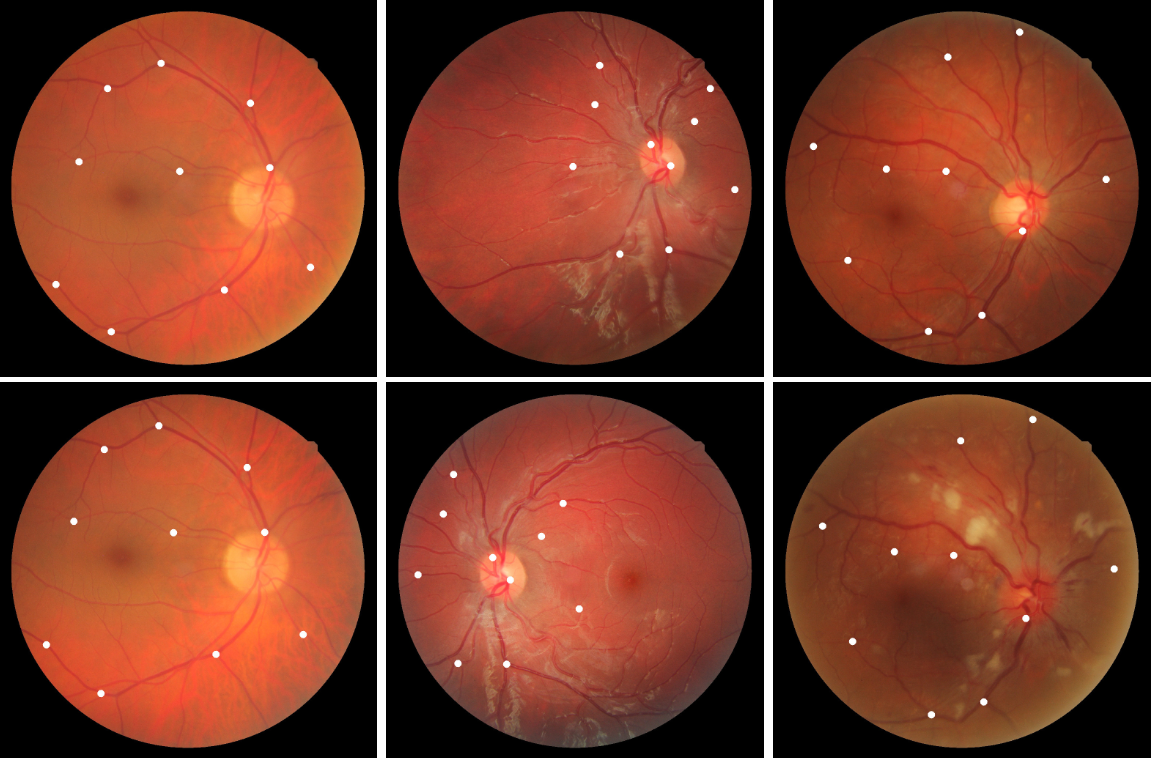
\includegraphics[width=0.8\textwidth]{imaxes/fire-ej.png}
    \caption{Ejemplo de imágenes del conjunto de datos FIRE \cite{FIRE} con los puntos de control indicados. De izquierda a derecha, categorías \textit{\textsf{S}}, \textit{\textsf{P}}, \textit{\textsf{A}} .}
    \label{fig:fire_ej}
\end{figure}

\subsection{RFMID}\label{subsec:RFMID}

El conjunto de datos RFMiD \cite{RFMiD} proporciona 3200 imágenes de fondo de ojo en color con resolución 1712x1712, etiquetadas según si tienen alguna anomalía o no.
También proporciona etiquetas para 45 diferentes anomalías anotadas por expertos.

Para utilizarlo en este trabajo, seleccionamos una submuestra y generamos transformaciones aleatorias. Guardamos las imágenes originales y las transformadas así como las matrices de transformación asociadas para la posterior evaluación.
También se divide entre transformaciones de color y de geometría.

En la figura \ref{fig:rfmid_ej} se muestra un ejemplo de una pareja de imágenes del conjunto de datos RFMiD.

\begin{figure}[tbp]
    \centering
    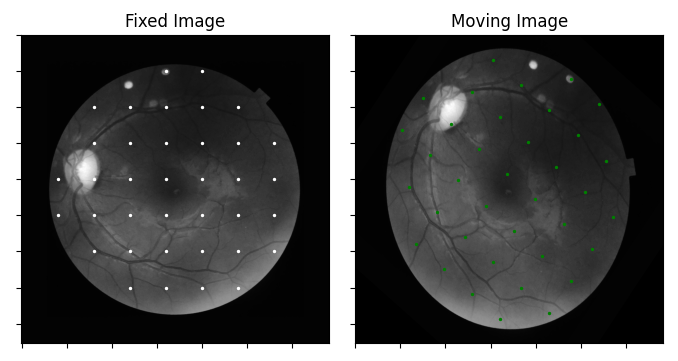
\includegraphics[width=0.8\textwidth]{imaxes/rfmid_ej.png}
    \caption{Ejemplo de imágenes del conjunto de datos RFMiD. La imagen de la izquierda es la fija y la de la derecha es la móvil.}
    \label{fig:rfmid_ej} 
\end{figure} 

\subsection{Diferencias entre los datasets}
\label{subsec:Diferencias entre os datasets}

Una ventaja de utilizar dos conjuntos de datos diferentes es que cada uno de ellos tiene características únicas que permiten evaluar el modelo en diferentes contextos.
La principal diferencia es que RMiFD es un conjunto de datos sintético, en el cual no introducimos diferencias de color y siempre tienen una superposición del 100\%, por lo que lo único que se evalúa es la capacidad del modelo para realizar los registros geométricos.
Por el contrario, FIRE es un conjunto de datos real, en el cual existen cambios en la iluminación, contraste, superposición y demás diferencias visuales, por lo que se evalúa la capacidad del modelo para realizar registros en condiciones mucho más adversas.

\section{Diseño de Experimentos}
\label{sec:Diseño de Experimentos}

El diseño de experimentos es un proceso sistemático que busca determinar la influencia de diferentes factores sobre un resultado específico. En este caso, el objetivo es evaluar cómo diferentes parámetros afectan a la calidad del registro de imágenes.

El coste computacional es un factor muy importante a tener en cuenta, ya que cada combinación de parámetros requiere un entrenamiento completo de la red por cada pareja de imágenes, lo que implica un alto coste energético y de tiempo.
Por ejemplo, para probar una combinación de parámetros sobre FIRE habrá que entrenar una red por cada pareja de imágenes de las 134 del conjunto de datos.
A un tiempo de entrenamiento de 3 minutos por pareja, el entrenamiento completo llevaría más de 6 horas por cada combinación de parámetros, con una huella de memoria de alrededor de 5 GB de VRAM.
El coste temporal y de memoria dependen de varios factores, siendo los más relevantes la regularización empleada, la resolución de la imagen, el tamaño del lote y la función de activación.
En concreto, SIREN tiene un coste computacional mucho mayor que ReLU, requiriendo alrededor del doble de tiempo y memoria para entrenar la red.

Debido al gran número de factores a tener en cuenta, se adoptó un enfoque de experimentación en fases.

Inicialmente se realizaron experimentos iniciales para identificar los rangos de parámetros más prometedores utilizando una submuestra representativa de 14 parejas de imágenes de cada categoría del dataset FIRE, con el objetivo: Reducir el espacio de parámetros para las fases posteriores.
En esta fase se evaluó la métrica de pérdida, la resolución de la imagen, la regularización empleada y el tamaño del lote.

Basándose en los resultados de la primera fase, se realizó una experimentación más exhaustiva para intentar mejorar el rendimiento del registro, centrándose en la estrategia de muestreo, la inicialización de los pesos de la red y un ajuste dinámico del tamaño de lote.

\subsection{Metodologías Desarrolladas}
\label{subsec:Metodoloxías Desenvoltas}

Para este trabajo tuvieron que desarrollarse varias metodologías específicas con el objetivo de mejorar el rendimiento del registro de imágenes de retina. Estas metodologías incluyen:

\subsubsection{Estrategias de Muestreo}
\label{subsubsec:estratexias_mostraxe}

\paragraph{Muestreo Inteligente}
En la estrategia de muestreo inteligente, se calcula una máscara de probabilidad para cada imagen, que se utiliza para seleccionar los puntos que se pasan a la red. Para calcular esta máscara, se extraen mediante operadores de Sobel los vasos sanguíneos y mediante umbralización el disco óptico. Estas son las zonas donde se espera que haya más información, y, por lo tanto, se les dan mayores probabilidades de ser seleccionadas.

\paragraph{Muestreo Ponderado}
Se implementó también una estrategia de muestreo ponderado, donde se seleccionan puntos aleatorios, pero con mayor probabilidad de que caigan en las zonas de interés (vasos sanguíneos y disco óptico), funcionando como un punto intermedio entre el muestreo aleatorio y el muestreo inteligente.

\paragraph{Muestreo Uniforme}
Se introdujo una estrategia de muestreo uniforme, donde se selecciona un número fijo de puntos en cada imagen, asegurando que están distribuidos uniformemente por toda la imagen. Es una estrategia similar al muestreo aleatorio, pero garantizando que se cubre la mayor parte posible de la imagen. Esto es relevante en experimentos con tamaños de lote pequeños, donde un muestreo aleatorio no tiene por qué cubrir todas las zonas de la imagen. Para implementarlo, se empleó una distribución basada en la rejilla de Fibonacci (Fibonacci lattice), que permite repartir los puntos de manera uniforme sobre la superficie circular de la retina. La posición de cada punto se calcula en coordenadas polares, asignando a cada punto un radio proporcional a la raíz cuadrada de su índice dividido por el número total de puntos, y un ángulo proporcional al índice multiplicado por $2\pi$ y dividido por el cuadrado del número áureo ($\varphi^2$):

\[
r_i = \sqrt{\frac{i}{N}}, \quad \theta_i = 2\pi \frac{i}{\varphi^2}
\]
donde $i$ es el índice del punto ($i = 1, \dots, N$), $N$ es el número total de puntos y $\varphi$ es el número áureo. De este modo, se consigue una cobertura uniforme y eficiente de la región de interés, evitando agrupamientos o zonas vacías.

En la figura \ref{fig:sampling_heatmaps} se pueden observar los diferentes tipos de muestreo utilizados.

\begin{figure}[tbp]
    \centering
    \begin{subfigure}[b]{0.3\textwidth}
        \centering
        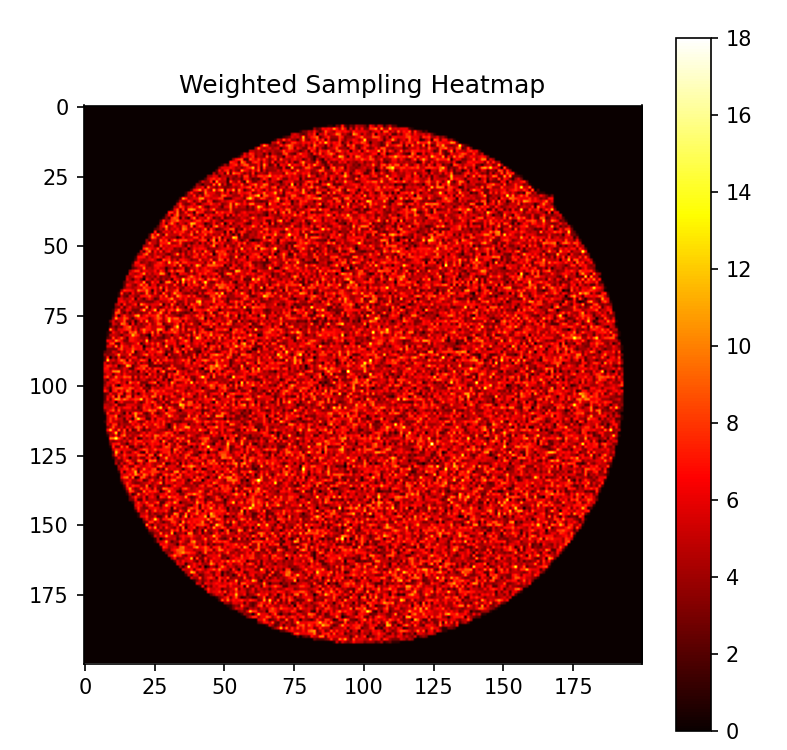
\includegraphics[width=\textwidth]{imaxes/muestraje/random_sampling_heatmap.png}
        \caption{Mapa de calor de muestreo aleatorio}
        \label{fig:random_sampling_heatmap}
    \end{subfigure}
    \hfill
    \begin{subfigure}[b]{0.3\textwidth}
        \centering
        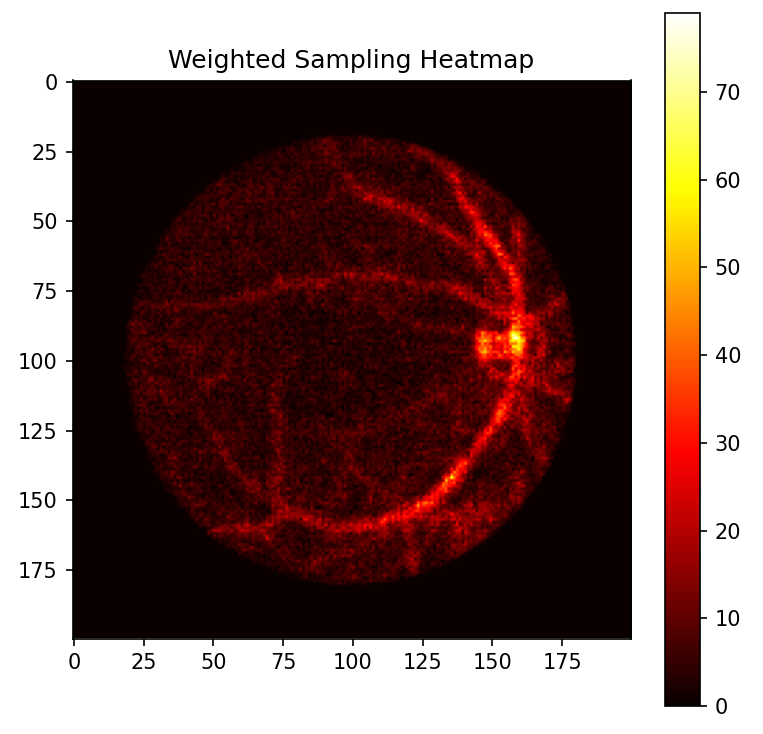
\includegraphics[width=\textwidth]{imaxes/muestraje/weighted_sampling_heatmap.png}
        \caption{Mapa de calor de muestreo ponderado}
        \label{fig:weighted_sampling_heatmap}
    \end{subfigure}
    \hfill
    \begin{subfigure}[b]{0.3\textwidth}
        \centering
        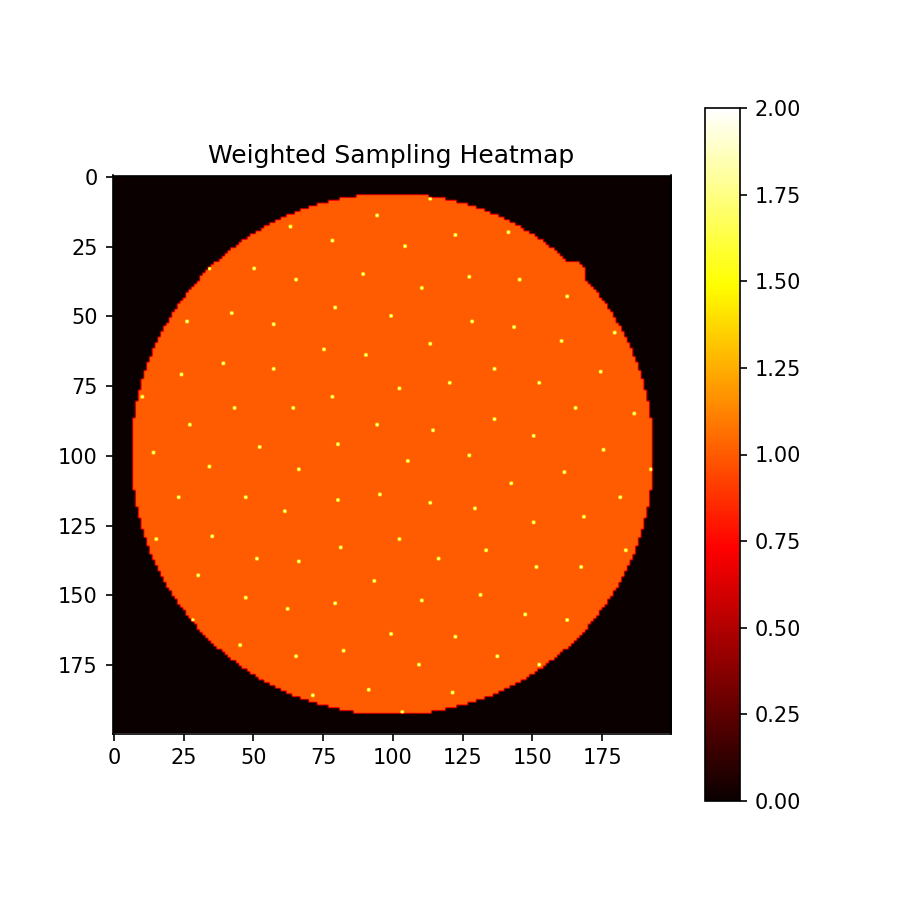
\includegraphics[width=\textwidth]{imaxes/muestraje/uniform_sampling_heatmap.png}
        \caption{Mapa de calor de muestreo uniforme (100 puntos)}
        \label{fig:uniform_sampling_heatmap}
    \end{subfigure}
    \caption{Mapas de calor que ilustran las diferentes estrategias de muestreo implementadas.}
    \label{fig:sampling_heatmaps}
\end{figure}

\subsubsection{Lotería de Inicialización}
\label{subsubsec:loteria_inicializacion}
Otra metodología diseñada fue la implementación de la lotería de inicialización. Esta técnica consiste en probar diferentes inicializaciones aleatorias de los pesos de la red para determinar cuál de ellas resulta más beneficiosa para la convergencia y el rendimiento final del modelo, y seleccionar la mejor inicialización para completar el entrenamiento.

\subsubsection{Ajuste Dinámico del Tamaño del Lote}
\label{subsubsec:axuste_dinamico_batch_size}
Se implementó el ajuste dinámico del tamaño del lote, que consiste en aumentar la cantidad de muestras tomadas por la red a lo largo del entrenamiento. Para llevar a cabo esta estrategia, se dividen las épocas en diferentes fases, donde cada fase hace uso de un tamaño de lote diferente, comenzando normalmente con tamaños más pequeños y aumentándolos progresivamente.

\section{Métodos de Evaluación}
\label{sec:Métodos de Evaluación}

La evaluación del rendimiento del sistema de registro constituye un aspecto fundamental para determinar la eficacia de las modificaciones implementadas.
El proceso de evaluación se divide en dos enfoques complementarios: la evaluación cuantitativa, que emplea métricas numéricas objetivas, y la evaluación cualitativa, que analiza los resultados de forma visual para detectar artefactos o deformaciones no deseadas que puedan escapar a las métricas numéricas.

Ambas evaluaciones son necesarias para obtener una visión completa de la calidad del registro, ya que la evaluación cuantitativa puede no ser suficiente para detectar problemas visuales que no se reflejen en las métricas.

\subsection{Evaluación Cuantitativa}\label{subsec:Avaliación Cuantitativa}

Utilizamos como método de evaluación cuantitativa el propuesto por FIRE \cite{FIRE}
generando un gráfico donde el eje x representa el valor del límite de error y el eje y muestra el porcentaje de pares de imágenes que fueron registrados con éxito para cada límite de error.

El error de registro se calcula mediante la distancia euclidiana media entre los puntos correspondientes en las imágenes fija y móvil:

\begin{figure}[tbp]
    \centering
    \[
    E = \frac{1}{N} \sum_{i=1}^{N} \left\| p_i^{\text{fixo}} - T(p_i^{\text{móbil}}) \right\|
    \]
    \caption{Cálculo del error de registro mediante la distancia euclidiana.}
    \label{fig:erro_registro}
\end{figure}

donde N es el número de puntos de referencia, p son las coordenadas de los puntos y T es la transformación aplicada.

Cuando el error de registro entre un par de imágenes está por debajo del umbral, se considera que el registro fue exitoso y viceversa. Esto da lugar a una curva monótona y continua que refleja la relación entre la tasa de éxito y la precisión objetivo, evitando así la necesidad de establecer un umbral arbitrario.
Estos gráficos se utilizan para ilustrar la precisión del registro tanto para casos individuales (donde se utilizan el porcentaje de parejas de puntos registrados con éxito)
como para el conjunto completo de datos.
Esta métrica facilita la comparación entre distintos métodos competidores y permite seleccionar el más adecuado según la precisión deseada.

Además, en FIRE la evaluación se segmentará en las 3 categorías de imágenes (S, P y A) para analizar el rendimiento del registro en cada una de ellas, ya que cada categoría presenta diferentes desafíos y características.

Mientras que FIRE ya provee los puntos de referencia para la evaluación, RFMID no lo hace.
Por lo tanto, para RFMID, utilizamos el mismo método de evaluación, pero generando los puntos manualmente de forma que cubran el interior de la máscara de la imagen fija (separados por 50 píxeles entre sí).

\begin{figure}[tbp]
    \centering
    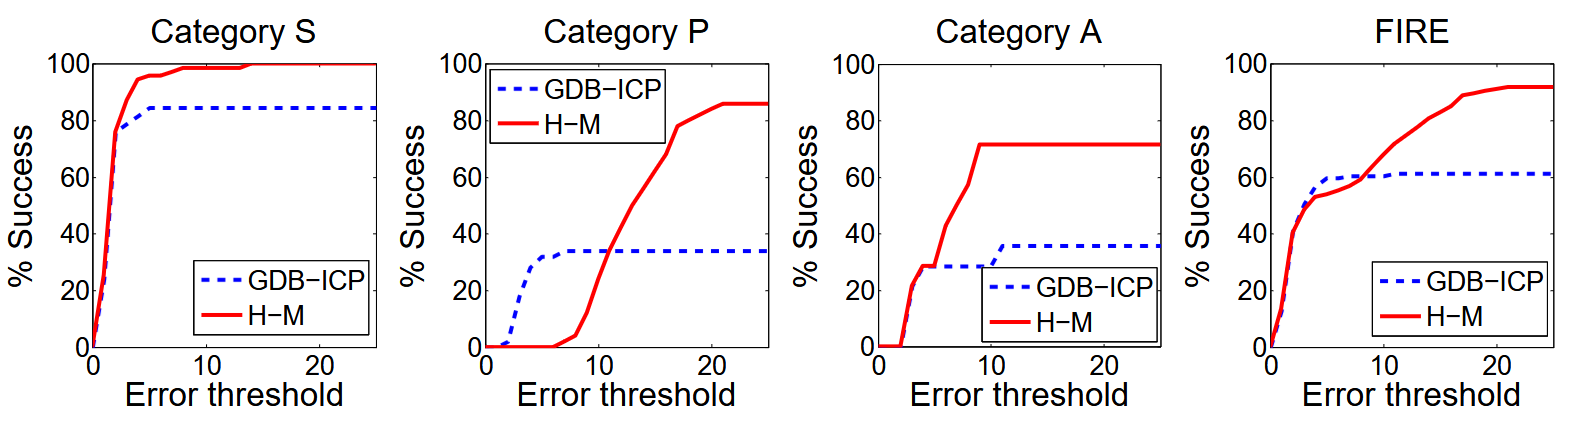
\includegraphics[width=0.8\textwidth]{imaxes/fire_aval.png}
    \caption{Gráfico de evaluación FIRE \cite{FIRE}}
    \label{fig:fire_aval}
\end{figure}

En el caso de RFMiD, dividiremos el conjunto de datos en varias categorías dependiendo de la dificultad del registro, que se calcula mediante la norma de Frobenius de una matriz $A \in \mathbb{R}^{m \times n}$.
Esta es una generalización de la distancia euclidiana aplicada a matrices, donde las imágenes con transformaciones más grandes se consideran más difíciles.

\begin{figure}[tbp]
    \centering
    \[
    \|A\|_F = \sqrt{\sum_{i=1}^{m} \sum_{j=1}^{n} |a_{ij}|^2}
    \]
    \caption{Norma de Frobenius de una matriz $A \in \mathbb{R}^{m \times n}$, donde $a_{ij}$ son los elementos de la matriz $A$.}
    \label{fig:frobenius_norm}
\end{figure}

En algunos casos también utilizaremos la distancia media entre los puntos correspondientes como métrica complementaria para evaluar la calidad del registro, ya que la tasa de éxito puede no ser suficiente para detectar los cambios.

\subsection{Evaluación Cualitativa}
\label{subsec:Avaliación Cualitativa}

En el caso de este trabajo, la evaluación cualitativa cobra gran importancia, ya que en la cuantitativa solo se está comparando sobre un número reducido de puntos en cada pareja de imágenes.
La evaluación visual permite detectar problemas que no se reflejen en las métricas cuantitativas, como artefactos visuales o deformaciones no deseadas,
especialmente en registros que tienen deformaciones locales que pueden no coincidir con ningún punto.

En el caso del dataset FIRE \cite{FIRE}, la evaluación visual es especialmente relevante, ya que tan solo se proporcionan 10 puntos de referencia por imagen, que pueden no ser suficientes para evaluar la calidad del registro en muchas zonas de la imagen.
Ya que en RFMID \cite{RFMiD} se utilizan puntos de referencia generados manualmente que cubren toda la imagen, la evaluación visual es algo menos relevante, ya que es más probable que una deformación local incorrecta sea detectada por algún punto y se vea reflejado en las métricas.

Con el objetivo de identificar fácilmente los distintos artefactos visuales o transformación no realista, se utilizan diferentes herramientas como la composición de imágenes, la visualización de los vectores de desplazamiento y la comparación de imágenes antes y después del registro.
En la figura \ref{fig:visex} se pueden observar algunos ejemplos de estas.

\begin{figure}[tbp]
    \centering
    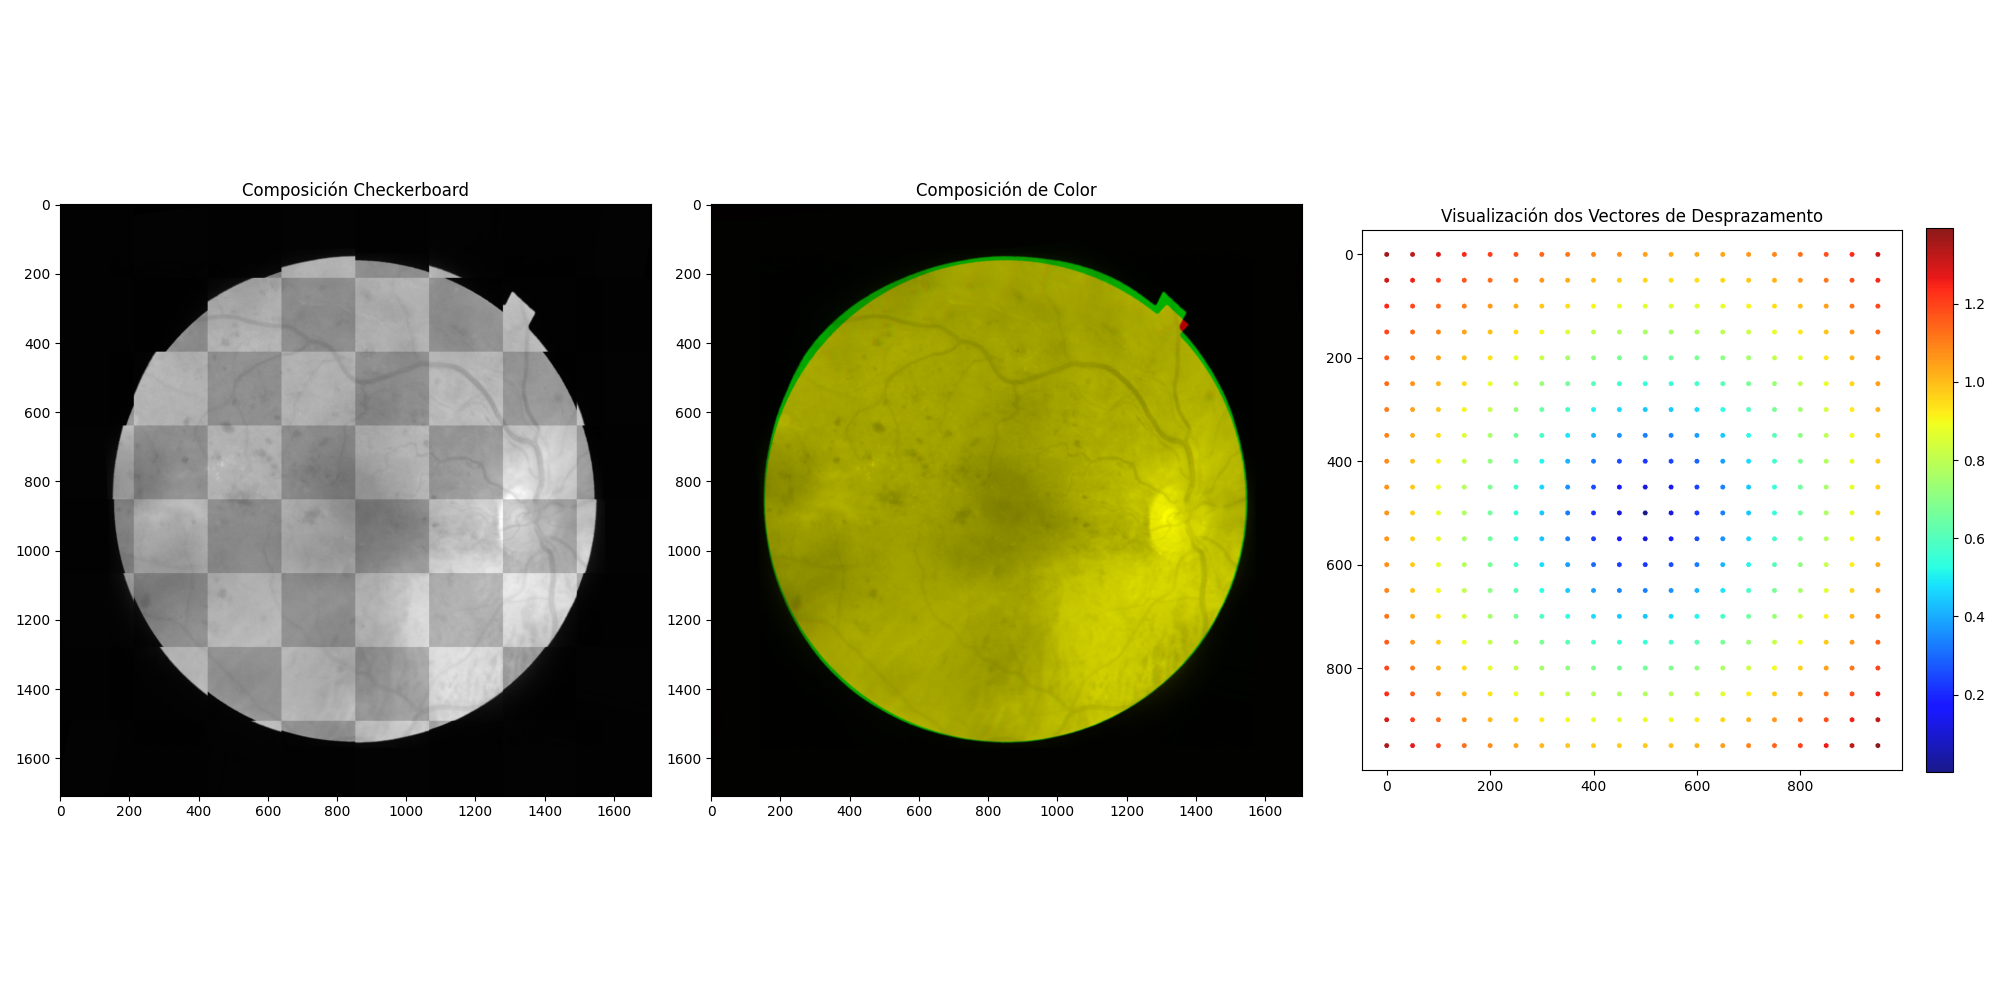
\includegraphics[width=0.9\textwidth]{imaxes/visex.png}
    \caption{Ejemplos de evaluación visual: (a) Composición de imágenes en checkerboard, (b) Composición de imágenes por color, (c) Visualización de los vectores de desplazamiento.}
    \label{fig:visex}
\end{figure}
 \chapter{Experimentos y resultados}
\label{chap:Experimentos e resultados}
\lettrine{E}{n} este capítulo se presentarán los experimentos realizados y los resultados obtenidos.
Para ello, se comenzará presentando una vista general del proceso de experimentación,
seguido de los propios experimentos realizados, para finalmente analizar los resultados obtenidos en conjunto y las conclusiones que se pueden extraer de ellos.

\section{Vista General}
\label{sec:Vista Xeral}

El objetivo del trabajo es determinar si las redes implícitas son aptas para la tarea de registro de retinas. La comparación principal se centra en la función de activación empleada (SIREN o ReLU), sobre los datasets FIRE y RFMID.

La evaluación inicial sobre el dataset FIRE, como se puede ver en las figuras \ref{fig:FIRE_relu} y \ref{fig:FIRE_SIREN}, mostró un rendimiento limitado. La categoría P resultó imposible de registrar, probablemente debido al bajo grado de superposición entre las imágenes (<75\%), mientras que las categorías S y A apenas alcanzaron tasas de éxito del 20\%.

Con el objetivo de mejorar este rendimiento y comprender los factores clave que influyen en el registro, se diseñó una serie de experimentos sistemáticos. Esta sección ofrece una panorámica de cada uno de estos experimentos, adelantando su motivación y sus hallazgos principales, que serán detallados en el resto del capítulo.

\begin{itemize}
\item \textbf{Función de pérdida:} La motivación era encontrar la métrica de similitud más robusta para las imágenes de retina, que presentan gran variabilidad en contraste e iluminación. El principal hallazgo fue que la elección óptima depende de la naturaleza de las imágenes: para imágenes reales con variabilidad (FIRE), las funciones basadas en características estructurales como NCC ofrecieron los mejores resultados; para imágenes sintéticas sin dicha variabilidad (RFMID), las funciones basadas en píxeles como L1 fueron superiores.

\item \textbf{Resolución de la imagen:} Se investigó si la alta resolución de las imágenes de retina (hasta 2160x2160) aportaba un beneficio significativo frente al coste computacional. La conclusión fue que, aunque resoluciones muy bajas eran insuficientes, no se observó una mejora notable por encima de 1250x1250 píxeles, estableciendo este valor como un buen equilibrio entre detalle y eficiencia.

\item \textbf{Regularización:} Este experimento fue crucial para evitar las deformaciones no realistas, un riesgo particular en los modelos SIREN debido a su sesgo hacia las altas frecuencias. Se confirmó que cierto grado de regularización es indispensable, pero la cantidad óptima de regularización no es universal, sino que depende de la complejidad de la transformación.

\item \textbf{Tamaño de lote:} El análisis cualitativo sugería que este era un parámetro de gran impacto. Los experimentos confirmaron que es uno de los factores más críticos para el éxito del registro. Un tamaño de lote grande (e.g., 10000 o más) es fundamental para obtener buenos resultados.

\item \textbf{Estrategias de muestreo:} La hipótesis inicial era que priorizar regiones con más información (vasos sanguíneos, disco óptico) mediante estrategias de muestreo "inteligentes" mejoraría el rendimiento. Los resultados demostraron que ninguna de las estrategias propuestas (uniforme, ponderada) ofreció una ventaja significativa sobre el muestreo aleatorio tradicional.

\item \textbf{Inicialización:} Dada la naturaleza no convexa del problema de optimización, se exploró si una selección cuidadosa de los pesos iniciales podría mejorar la convergencia. Se implementó una "lotería de inicialización" que escoge la mejor de varias ejecuciones iniciales. Se observó una mejora marginal pero consistente, indicando que la inicialización tiene cierto impacto, aunque no es un factor transformador.

\item \textbf{Ajuste dinámico del tamaño de lote:} Se probó la estrategia de comenzar con un tamaño de lote pequeño para aprender la transformación global y luego aumentarlo para refinar detalles locales. El resultado fue concluyente y contrario a la hipótesis: esta estrategia resultó ser perjudicial, empeorando el rendimiento. Un tamaño de lote grande y constante desde el inicio demostró ser más eficaz.

\end{itemize}

A menos que se especifique lo contrario, para los experimentos se utilizará un learning rate de 0.0001, tamaño de lote de 10000 puntos y 1500 épocas. Estos valores se determinaron a partir de los utilizados originalmente por IDIR y del análisis cualitativo de los resultados obtenidos en experimentos preliminares. El conjunto de estos experimentos permite construir una comprensión detallada de las fortalezas y debilidades de las redes implícitas en esta tarea.

\begin{figure}[tbp]
    \centering
    \begin{subfigure}[b]{0.5\textwidth}
        \centering
        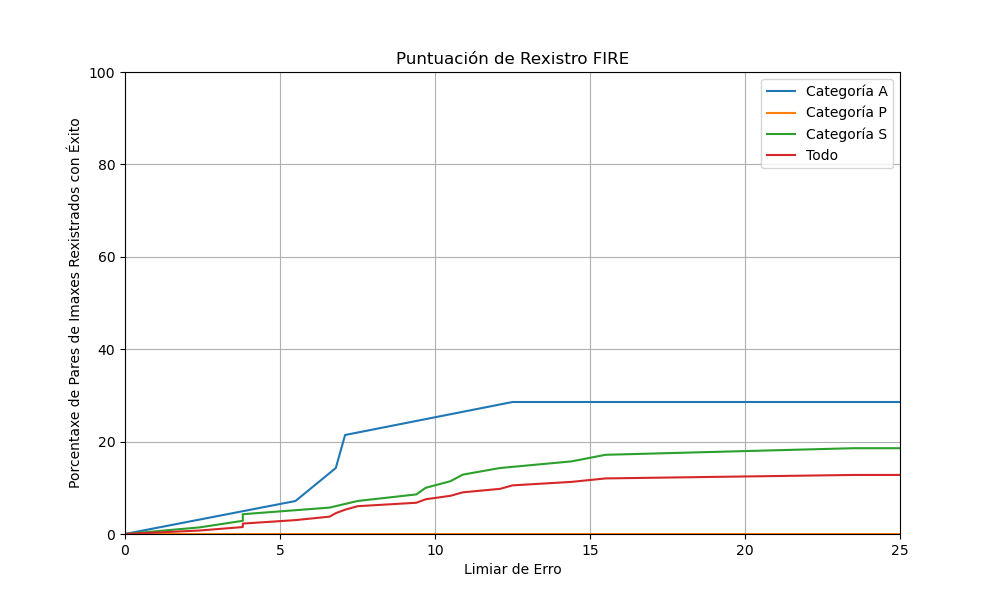
\includegraphics[width=\textwidth]{imaxes/FIRE_scores/fire_registration_score_ReLU.png}
        \caption{Métrica FIRE, función de activación ReLU}
        \label{fig:FIRE_relu}
    \end{subfigure}\hfill
    \begin{subfigure}[b]{0.5\textwidth}
        \centering
        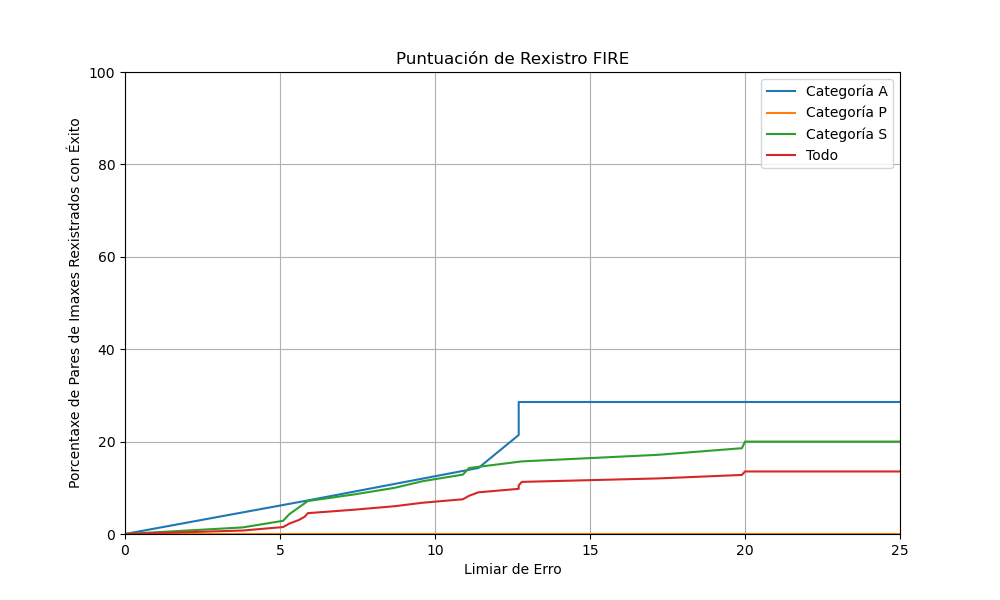
\includegraphics[width=\textwidth]{imaxes/FIRE_scores/fire_registration_scores_SIREN.png}
        \caption{Métrica FIRE, función de activación SIREN}
        \label{fig:FIRE_SIREN}
    \end{subfigure}
    \caption{Métricas dataset FIRE}
    \label{fig:FIRE_scores}
\end{figure}

\subsection{Descripción de los experimentos}
\label{subsec:Descrición dos experimentos}

\textbf{Experimentos iniciales:} En esta parte se realizarán experimentos para determinar unos valores aceptables para los parámetros de la red en el contexto de la imagen oftalmológica,
así como determinar su influencia en el rendimiento de la red.

\begin{itemize}
    \item \textbf{Función de pérdida:} Debido a las características únicas de las imágenes de retina, con variabilidad en iluminación y contraste, es crucial determinar qué función de pérdida es más robusta para esta tarea. Se compararon funciones basadas en píxeles (MSE, L1) con funciones basadas en características estructurales (NCC, SSIM) para determinar cuál captura mejor las correspondencias entre imágenes retinianas.
    \item \textbf{Resolución de la imagen:} Las imágenes de retina pueden tener resoluciones de hasta 2160×2160 píxeles, significativamente mayores que las imágenes de pulmón utilizadas originalmente por IDIR (512×512). Es necesario determinar si una mayor resolución mejora el rendimiento o si introduce ruido que perjudica el registro.
    \item \textbf{Regularización:} SIREN tiene un sesgo inherente hacia señales de alta frecuencia, lo que puede provocar sobreajuste. Se evalúa el impacto de diferentes términos de regularización (jacobiana, hiperelástica, energía de flexión) para determinar los valores óptimos que eviten deformaciones no realistas.
    \item \textbf{Tamaño de lote:} La densidad de puntos mostrados a la red puede ser crucial para el éxito del registro. Tamaños de lote mayores proporcionan más información por iteración, pero a un mayor coste computacional. Se investiga el equilibrio óptimo entre eficiencia y rendimiento.
\end{itemize}

\textbf{Estrategias de muestreo:} Las imágenes de retina tienen zonas con diferentes cantidades de información estructural (vasos sanguíneos, disco óptico vs. fondo uniforme). Se comparan estrategias de muestreo aleatorio, uniforme y ponderado por contenido para determinar si priorizar ciertas regiones mejora el registro.

\textbf{Inicialización:} La naturaleza no convexa de la función de pérdida puede hacer que diferentes inicializaciones converjan a mínimos locales distintos. Se implementó una lotería de inicialización para seleccionar la inicialización más prometedora basándose en la pérdida inicial.

\textbf{Ajuste dinámico del tamaño de lote:} Se teoriza que la red podría beneficiarse de aprender primero transformaciones globales con tamaños de lote pequeños y después refinar con mayores cantidades de puntos mostrados para capturar detalles locales.

\section{Ejemplos de registro}\label{sec:Ejemplos de registro}

Diferentes ejemplos de registro, tanto exitosos como fallidos, se pueden observar en la figura \ref{fig:reg_examples}.
La primera imagen corresponde con la imagen fija, la segunda corresponde con la imagen registrada, la tercera con la imagen móvil y la cuarta el campo de deformación aplicado a una rejilla cuadrada.

Se pueden observar los puntos de control, siendo los blancos los de la imagen fija, los verdes los de la imagen móvil y los azules los desplazados por la red.
\begin{figure}[tbp]
    \centering
    \begin{subfigure}[b]{0.45\textwidth}
        \centering
        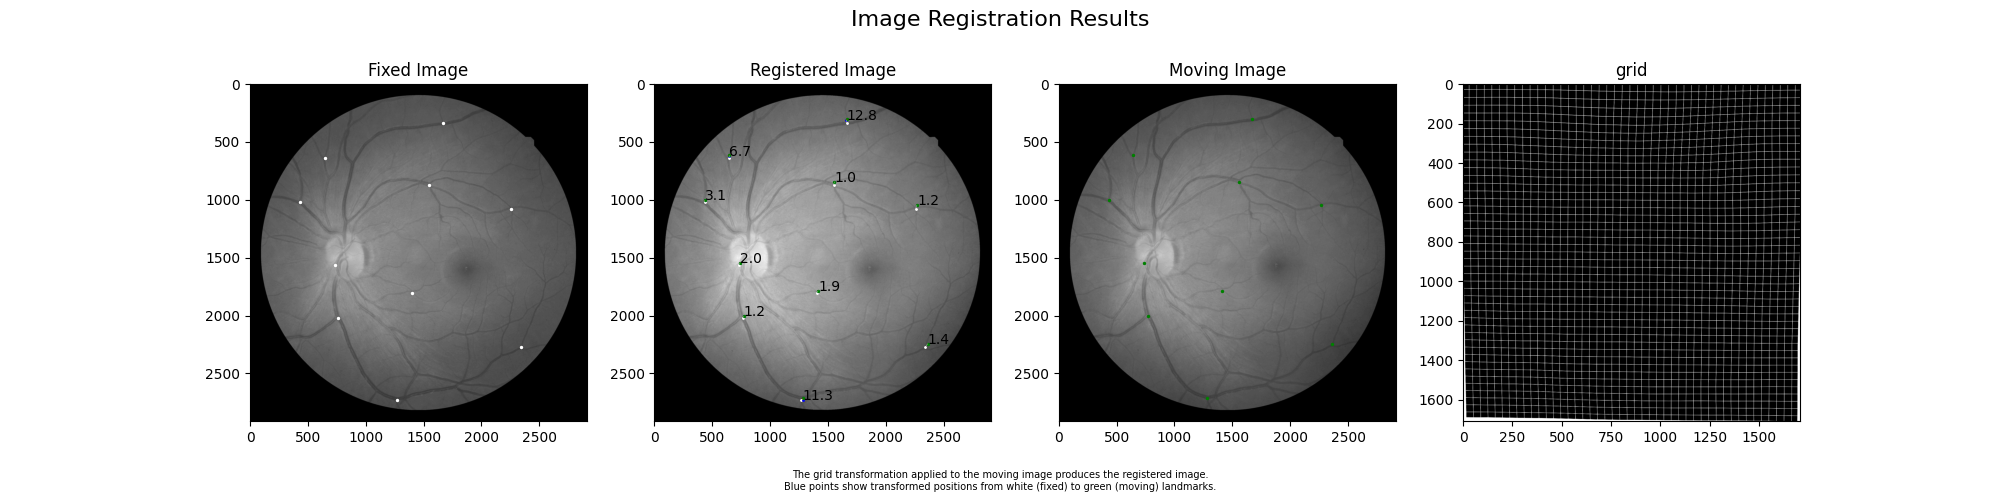
\includegraphics[width=\textwidth]{imaxes/reg_examples/FIRE_MLP_buena.png}
        \caption{Registro exitoso de un par de imágenes del dataset FIRE con la función de activación ReLU}
        \label{fig:reg_example_FIRE_MLP_buena}
    \end{subfigure}\hfill
    \begin{subfigure}[b]{0.45\textwidth}
        \centering
        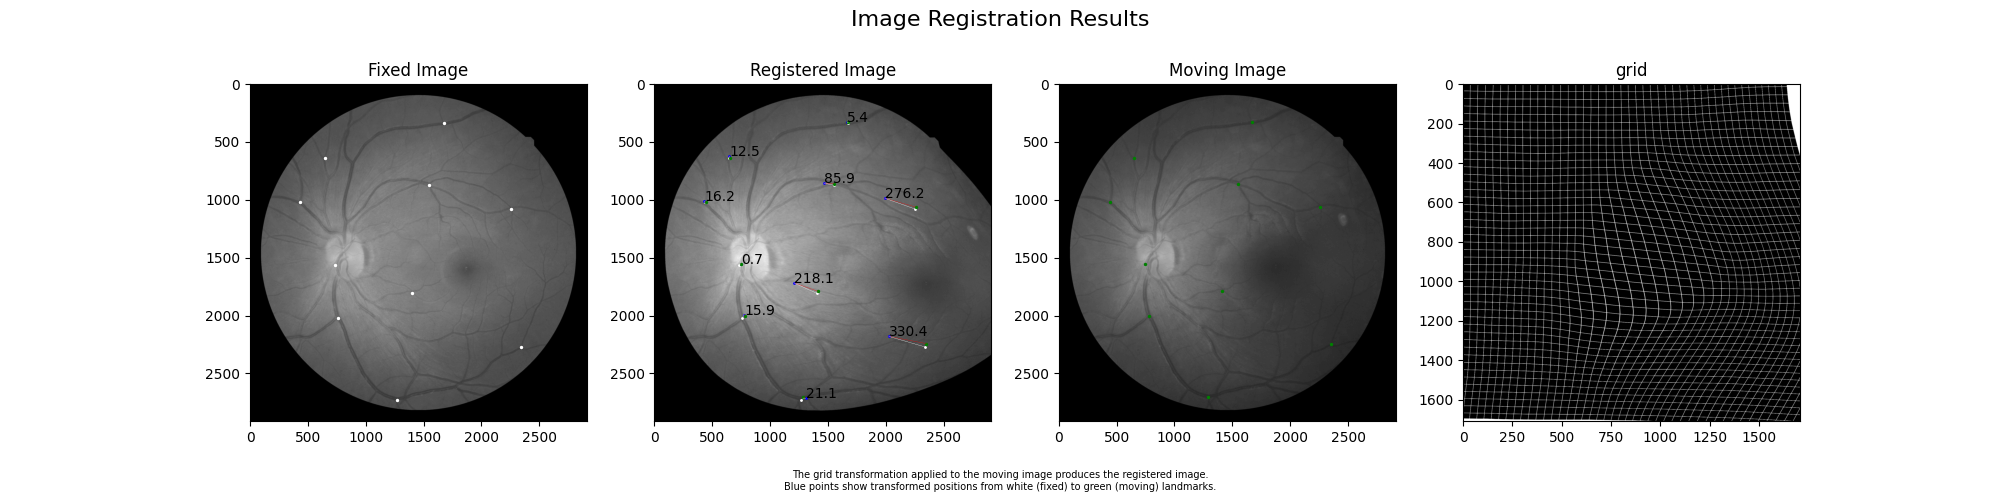
\includegraphics[width=\textwidth]{imaxes/reg_examples/FIRE_MLP_mala.png}
        \caption{Registro fallido de un par de imágenes del dataset FIRE con la función de activación ReLU}
        \label{fig:reg_example_FIRE_MLP_mala}
    \end{subfigure}

    \vskip\baselineskip

    \begin{subfigure}[b]{0.45\textwidth}
        \centering
        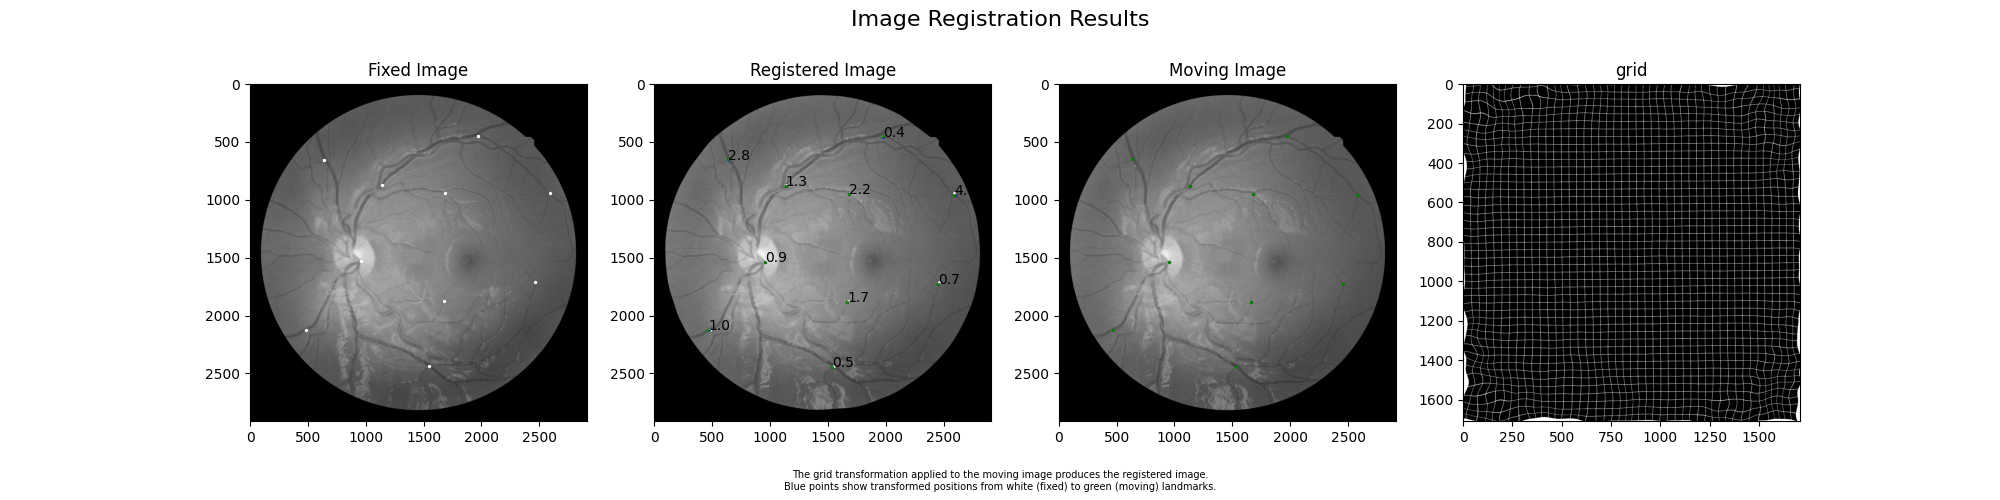
\includegraphics[width=\textwidth]{imaxes/reg_examples/FIRE_SIREN_buena.png}
        \caption{Registro exitoso de un par de imágenes del dataset FIRE con la función de activación SIREN}
        \label{fig:reg_example_FIRE_SIREN_buena}
    \end{subfigure}\hfill
    \begin{subfigure}[b]{0.45\textwidth}
        \centering
        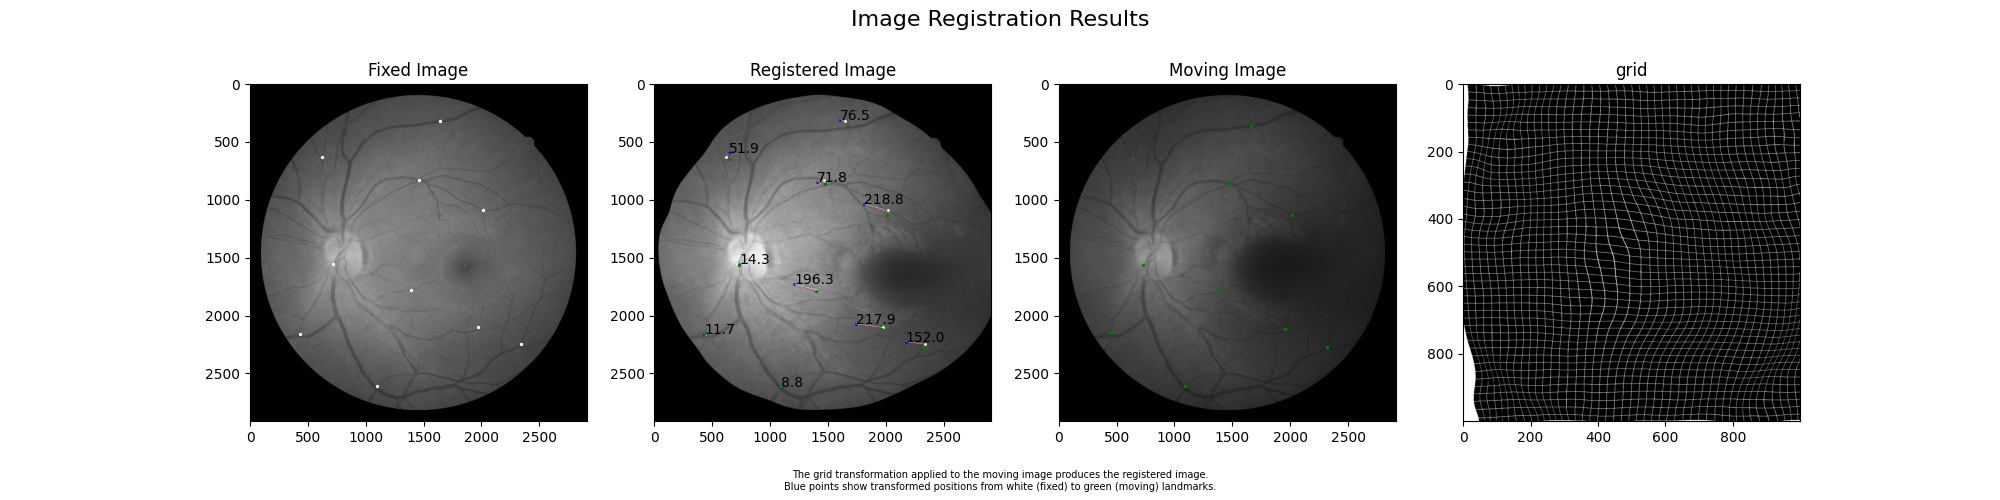
\includegraphics[width=\textwidth]{imaxes/reg_examples/FIRE_SIREN_mala.png}
        \caption{Registro fallido de un par de imágenes del dataset FIRE con la función de activación SIREN}
        \label{fig:reg_example_FIRE_SIREN_mala}
    \end{subfigure}

    \vskip\baselineskip

    \begin{subfigure}[b]{0.45\textwidth}
        \centering
        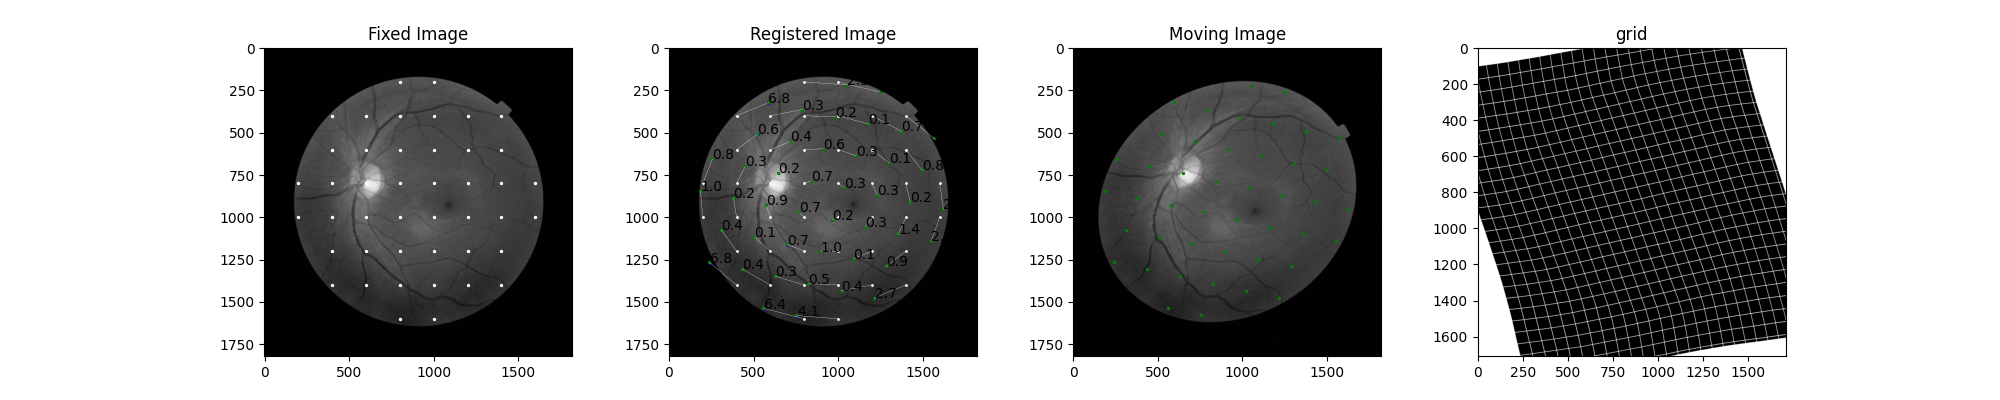
\includegraphics[width=\textwidth]{imaxes/reg_examples/RFMID_MLP_buena.png}
        \caption{Registro exitoso de un par de imágenes del dataset RFMID con la función de activación ReLU}
        \label{fig:reg_example_RFMID_MLP_buena}
    \end{subfigure}\hfill
    \begin{subfigure}[b]{0.45\textwidth}
        \centering
        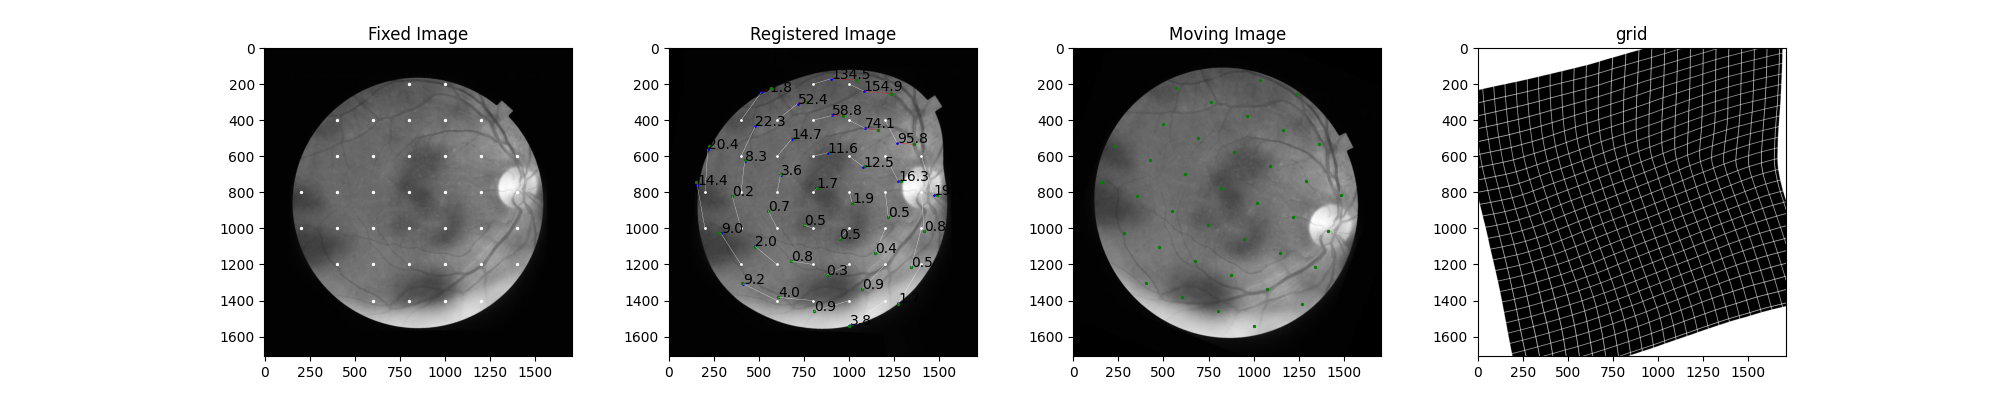
\includegraphics[width=\textwidth]{imaxes/reg_examples/RFMID_MLP_mala.png}
        \caption{Registro fallido de un par de imágenes del dataset RFMID con la función de activación ReLU}
        \label{fig:reg_example_RFMID_MLP_mala}
    \end{subfigure}

    \vskip\baselineskip

    \begin{subfigure}[b]{0.45\textwidth}
        \centering
        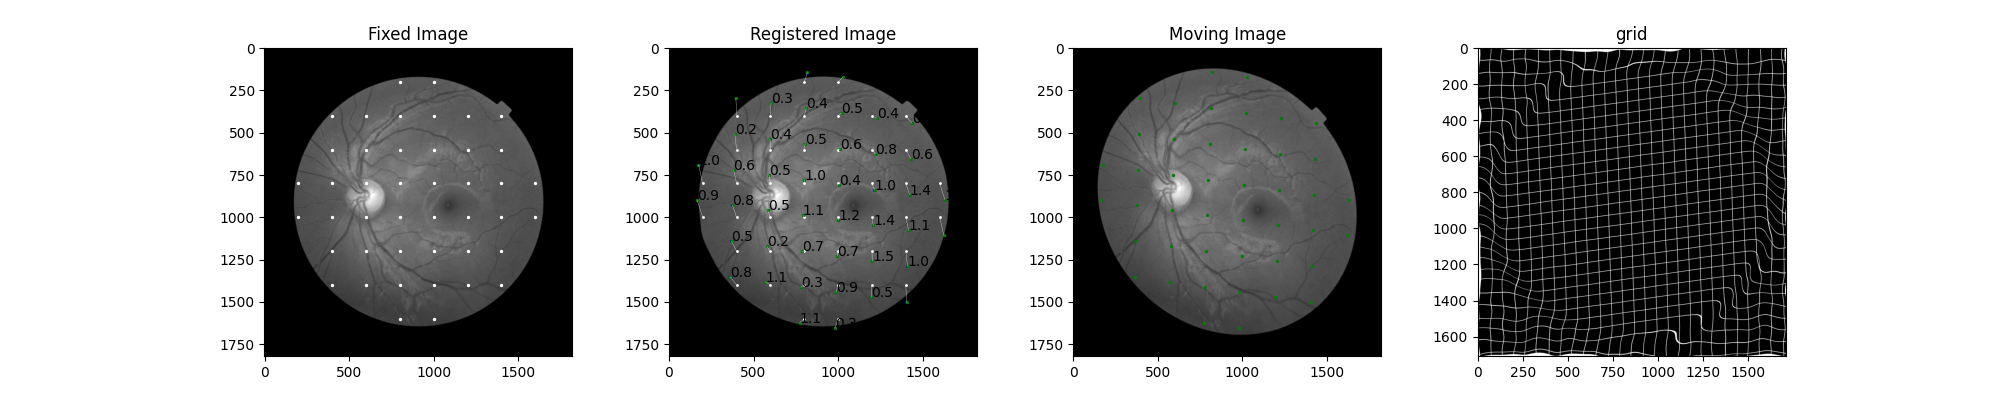
\includegraphics[width=\textwidth]{imaxes/reg_examples/RFMID_SIREN_buena.png}
        \caption{Registro exitoso de un par de imágenes del dataset RFMID con la función de activación SIREN}
        \label{fig:reg_example_RFMID_SIREN_buena}
    \end{subfigure}\hfill
    \begin{subfigure}[b]{0.45\textwidth}
        \centering
        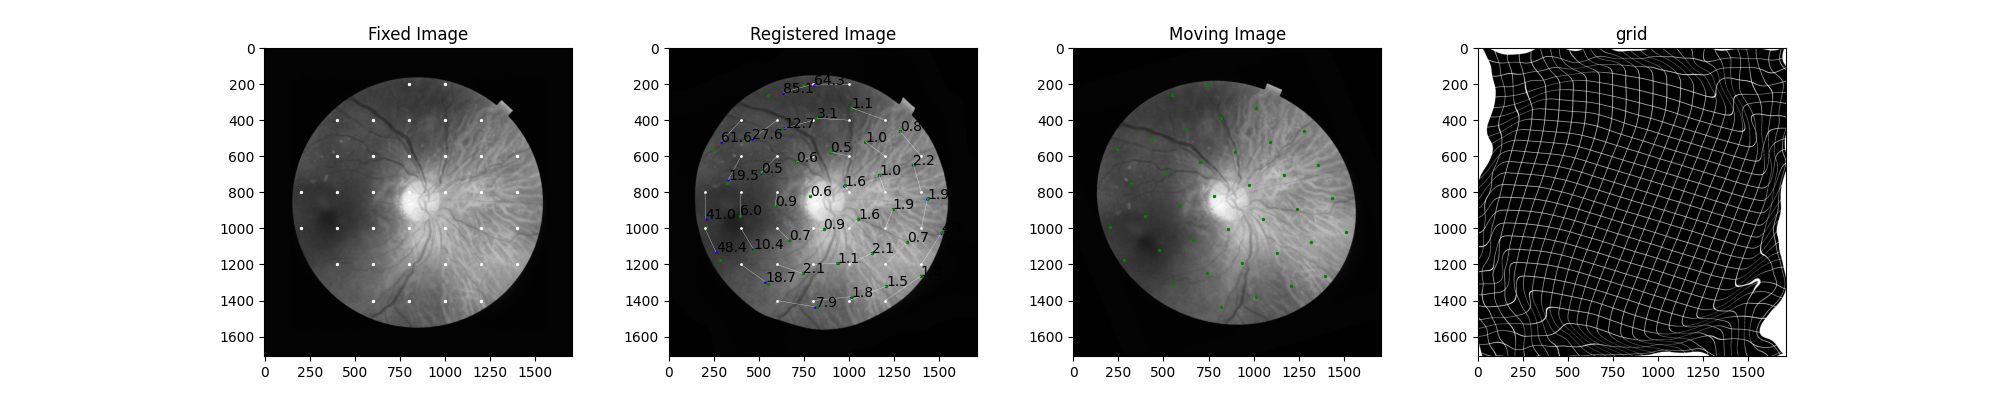
\includegraphics[width=\textwidth]{imaxes/reg_examples/RFMID_SIREN_mala.png}
        \caption{Registro fallido de un par de imágenes del dataset RFMID con la función de activación SIREN}
        \label{fig:reg_example_RFMID_SIREN_mala}
    \end{subfigure}

    \caption{Ejemplos de registro: combinaciones de dataset (FIRE/RFMID), función de activación (relu/SIREN) y éxito.}
    \label{fig:reg_examples}
\end{figure}

\section{Función de pérdida}
\label{sec:Función de pérdida}

\subsection{Planteamiento}
\label{subsec:Planteamiento-perda}

Las funciones de pérdida valoradas para este trabajo ya fueron explicadas en la sección \ref{subsubsec:Termos de Perda}.

Para determinar cuál es la función de pérdida más adecuada para la tarea de registro de retinas, se realizaron experimentos comparando el rendimiento de cada una sobre una muestra de imágenes de los datasets de FIRE y RFMID.
Ya que la red no es capaz de registrar con éxito gran parte de las imágenes en estas condiciones, se tomará la distancia media de todos los puntos como métrica de comparación.

\subsection{Resultados}
\label{subsec:Resultados-perda}

Se presenta en la figura \ref{fig:loss_functions_comparison} la comparación entre las diferentes funciones de pérdida.

\begin{figure}[tbp]
    \centering
    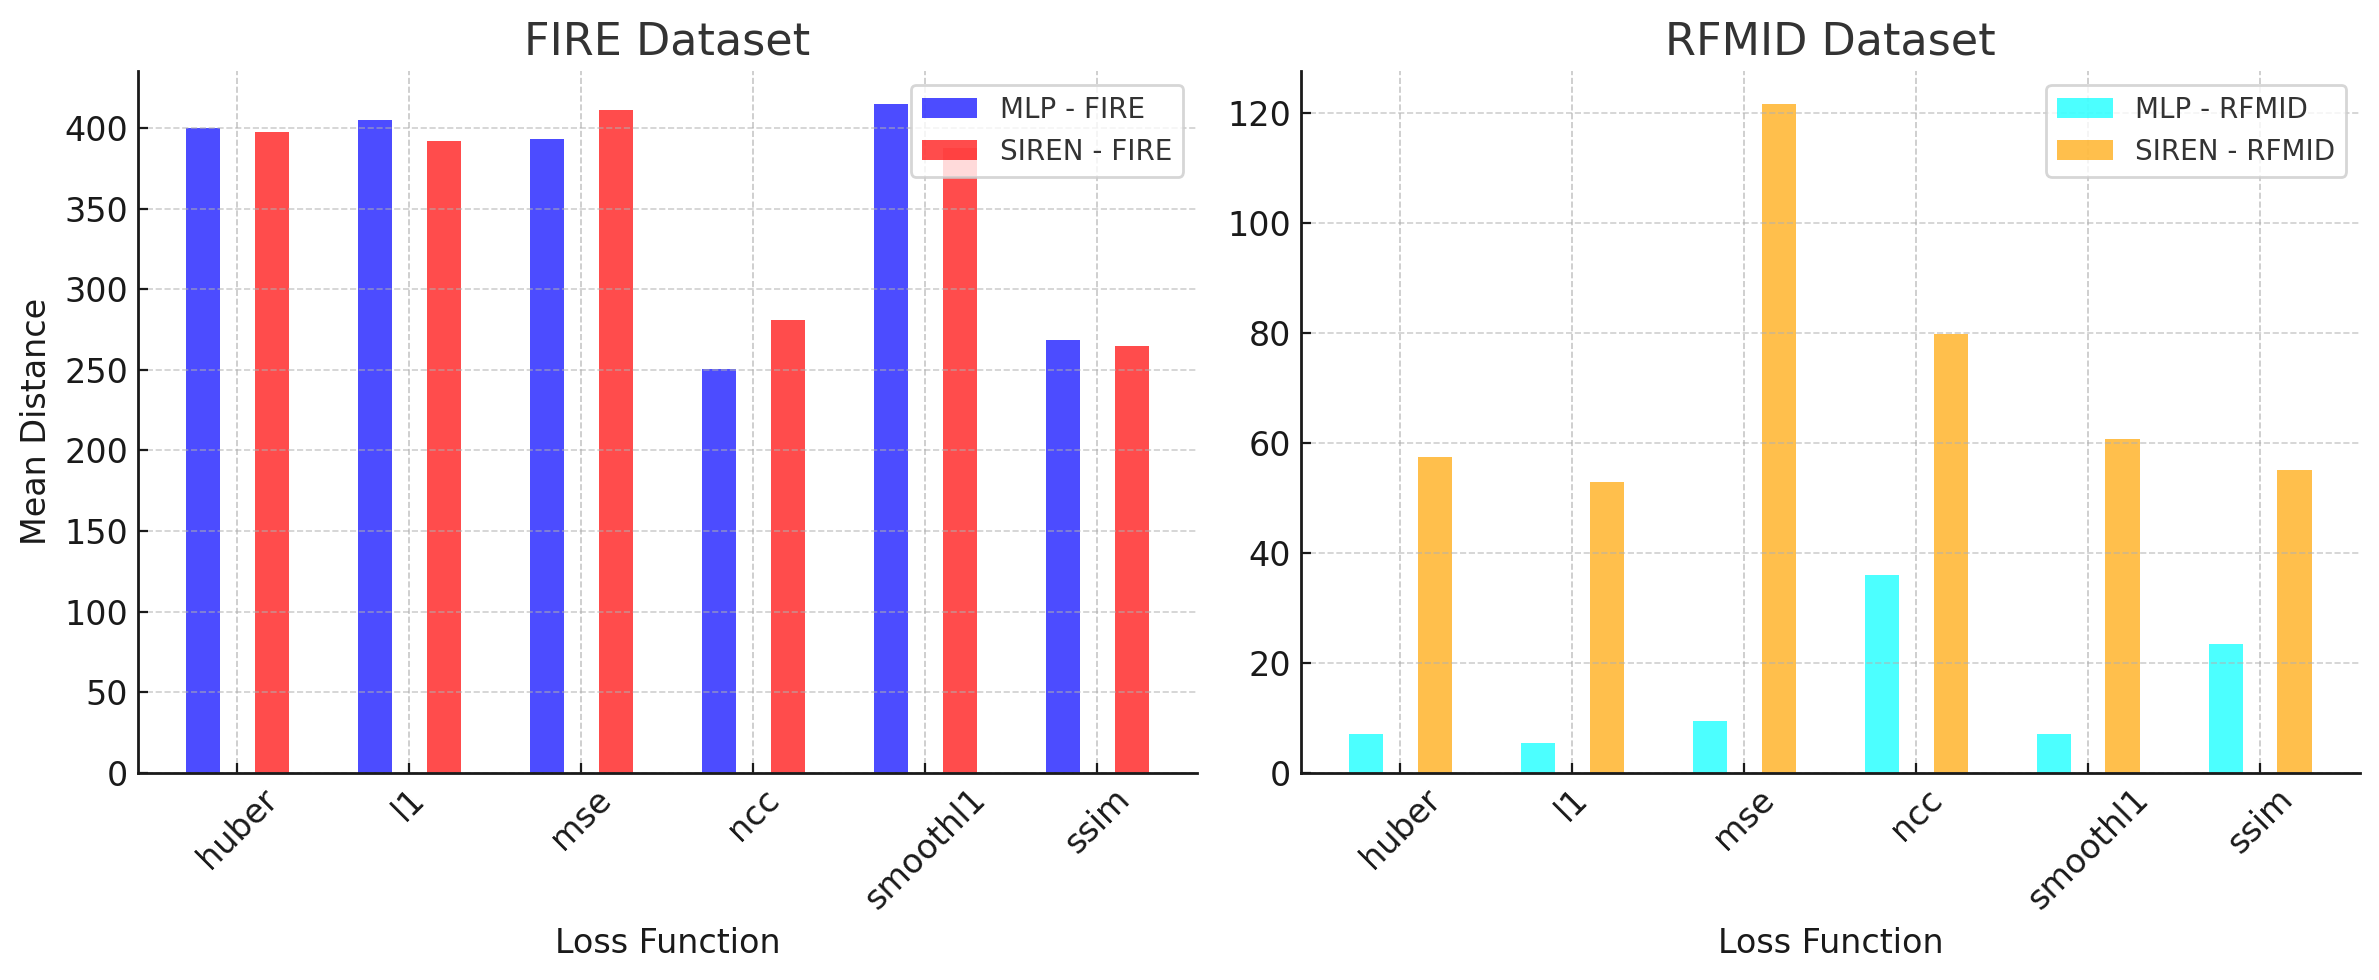
\includegraphics[width=1\textwidth]{imaxes/losstype.png}
    \caption{Comparación de diferentes funciones de pérdida sobre imágenes de FIRE y RFMID}
    \label{fig:loss_functions_comparison}
\end{figure}

\subsection{Discusión}
\label{subsec:Discusion-loss}

Se observa cómo las métricas que tienen en cuenta la estructura de la imagen (NCC, SSIM) tienden a dar mejores resultados que aquellas que no lo hacen (MSE, Huber, Smooth L1) con el dataset de FIRE, mientras que con RFMID ocurre lo contrario.
Esto puede deberse a que las imágenes reales de retina tienen una mayor variabilidad en la iluminación y contraste, por lo que las métricas que no tienen en cuenta la estructura de la imagen serán menos robustas a estas diferencias.
En el caso de RFMID, al ser imágenes sintéticas, la variabilidad en la iluminación y contraste es nula, lo que explica los mejores resultados de las métricas que no tienen en cuenta la estructura de la imagen.
De la misma forma, la función de activación Relu tiende a producir funciones predominantemente lineales, lo que se adapta mejor a las transformaciones realizadas en el dataset RFMID.

SSIM es menos robusta al ruido y sensible al tamaño de las secciones utilizadas, así como computacionalmente costosa. Además, tiene otro coste añadido ya que no es posible calcular SSIM tan solo comparando los puntos mostrados ya que utiliza ventanas deslizantes para evaluar luminancia, contraste y estructura.
Para utilizarla es necesario reconstruir la imagen en cada iteración lo que tiene un alto coste computacional.
En el caso de no reconstruir la imagen y utilizar los puntos mostrados directamente, esta métrica funciona igualmente pero con resultados ligeramente peores, ya que pierde toda su capacidad de capturar variaciones locales de luminancia, contraste y estructura, lo que se traduce en una función de pérdida global sin consideraciones locales.

\subsection{Conclusiones}
\label{subsec:Conclusions-loss}

En base a los resultados obtenidos, se pueden extraer las siguientes conclusiones:
\begin{itemize}
    \item Para el dataset FIRE, que contiene imágenes reales de retina con variabilidad en iluminación y contraste, las funciones de pérdida basadas en características estructurales como NCC y SSIM proporcionan resultados significativamente mejores.
    \item Para el dataset RFMID, que contiene imágenes con tan solo variación geométrica, las funciones de pérdida basadas en píxeles como L1 y Huber ofrecen mejores resultados.
    \item Se observa una diferencia sistemática entre los modelos Relu y SIREN, siendo los primeros más efectivos para el dataset RFMID, mientras que ambos muestran rendimientos comparables para FIRE.
\end{itemize}

\section{Resolución de la imagen}
\label{sec:Resolución de la imagen}

\subsection{Planteamiento}
\label{subsec:Planteamiento-resolution}

Para determinar cuál es la resolución más adecuada, se realizaron experimentos comparando el rendimiento de cada una sobre una muestra de imágenes de los datasets de FIRE y RFMID.
Debido a que la red no es capaz de registrar con éxito gran parte de las imágenes, se tomará la distancia media de todos los puntos como métrica de comparación.

La resolución de la imagen influye de forma directa en el resto de parámetros de la red.
Por ejemplo, un tamaño de lote de 1000 puntos en una imagen de 256x256 es una densidad de puntos mucho mayor que en una imagen de 1024x1024.

Además, la resolución de la imagen también influye en la capacidad de la red para aprender las transformaciones, ya que la información que recibe es más detallada.
Esto puede ser beneficioso si estos detalles contienen información relevante para la tarea de registro, pero también podría ser perjudicial si contienen una gran parte de ruido.

El tamaño de las imágenes también es una de las principales diferencias entre las imágenes de retina y las de pulmones utilizadas originalmente por IDIR, teniendo estas últimas de 512x512 mientras que las imágenes de los ojos cuentan con resoluciones de hasta 2160x2160.

\subsection{Resultados}\label{subsec:Resultados-resolution}

Se presenta en la figura \ref{fig:resoluciónchart} la comparación entre las diferentes resoluciones.

\begin{figure}[tbp]
    \centering
    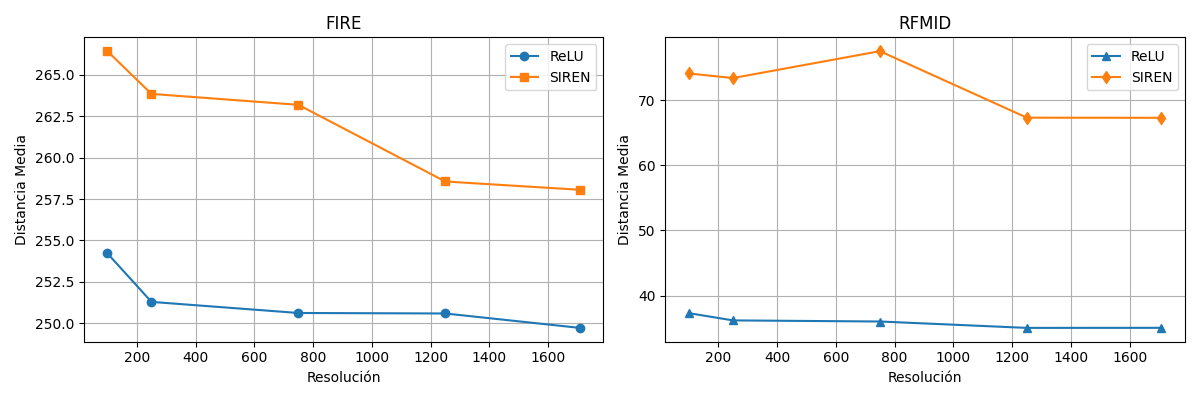
\includegraphics[width=1\textwidth]{imaxes/resolutionchart.png}
    \caption{Comparación de diferentes resoluciones de pérdida sobre imágenes de FIRE y RFMID. Menor distancia media es mejor.}
    \label{fig:resoluciónchart}
\end{figure}

\subsection{Discusión}
\label{subsec:Discusion-resolution}

Se puede observar cómo una mayor resolución tiende a dar ligeramente mejores resultados, pero a un coste computacional mayor.
Esto puede deberse a la precisión con la que se hace la evaluación más que a una mejor capacidad de la red para aprender las transformaciones, ya que las diferencias son muy pequeñas y consistentes entre los diferentes pares de imágenes.
Esto sugiere que la resolución no tiene un impacto significativo en el rendimiento de la red, y que la mayoría de la información relevante para la tarea de registro ya está capturada en resoluciones inferiores.

\subsection{Conclusiones}
\label{subsec:Conclusions-resolution}

Basándonos en los resultados obtenidos, podemos concluir que:

1. Resoluciones inferiores a 100×100 no capturan suficientes detalles de las estructuras vasculares retinianas para realizar un registro preciso, especialmente en imágenes reales del dataset FIRE.

2. Aumentar la resolución por encima de 1250x1250 no aporta beneficios significativos.

Para los experimentos subsiguientes, se adoptará una resolución estándar de 1250x1250 píxeles, que demostró proporcionar un buen balance entre rendimiento y eficiencia computacional.

\section{Regularización}
\label{sec:Regularización}

\subsection{Planteamiento}
\label{subsec:Planteamento-regularization}

Para determinar cuál es la cantidad de regularización óptima, se realizaron experimentos comparando el rendimiento de cada una sobre una muestra de imágenes de los datasets de FIRE y RFMID con las diferentes funciones de activación y diferentes grados de regularización.

El proceso de regularización ayuda a la red a evitar el sobreajuste, modificando el término de pérdida para penalizar las transformaciones poco realistas.
Las técnicas de regularización valoradas, que ya fueron explicadas en detalle en la sección \ref{subsubsec:Termos de regularización}

Los valores utilizados para cada tipo de regularización se ajustaron a partir de los utilizados originalmente por IDIR y comparado el impacto de cada uno de ellos sobre la función de pérdida, ya que la escala de cada uno de ellos es diferente.

En el anexo \ref{sec:Anexo regularization} se detalla una búsqueda más completa para explorar las relaciones entre los diferentes tipos de regularización.
En este apartado solo se presentarán los resultados de los experimentos realizados con la regularización hiperelástica, que se considera la más relevante para esta tarea.

\subsection{Resultados}
\label{subsec:Resultados-regularization}

La comparación entre los diferentes valores de regularización hiperelástica se presenta en la figura \ref{fig:barplot_hyper_reg_comparison}.

\begin{figure}[tbp]
    \centering
    \begin{subfigure}[b]{0.48\textwidth}
        \centering
        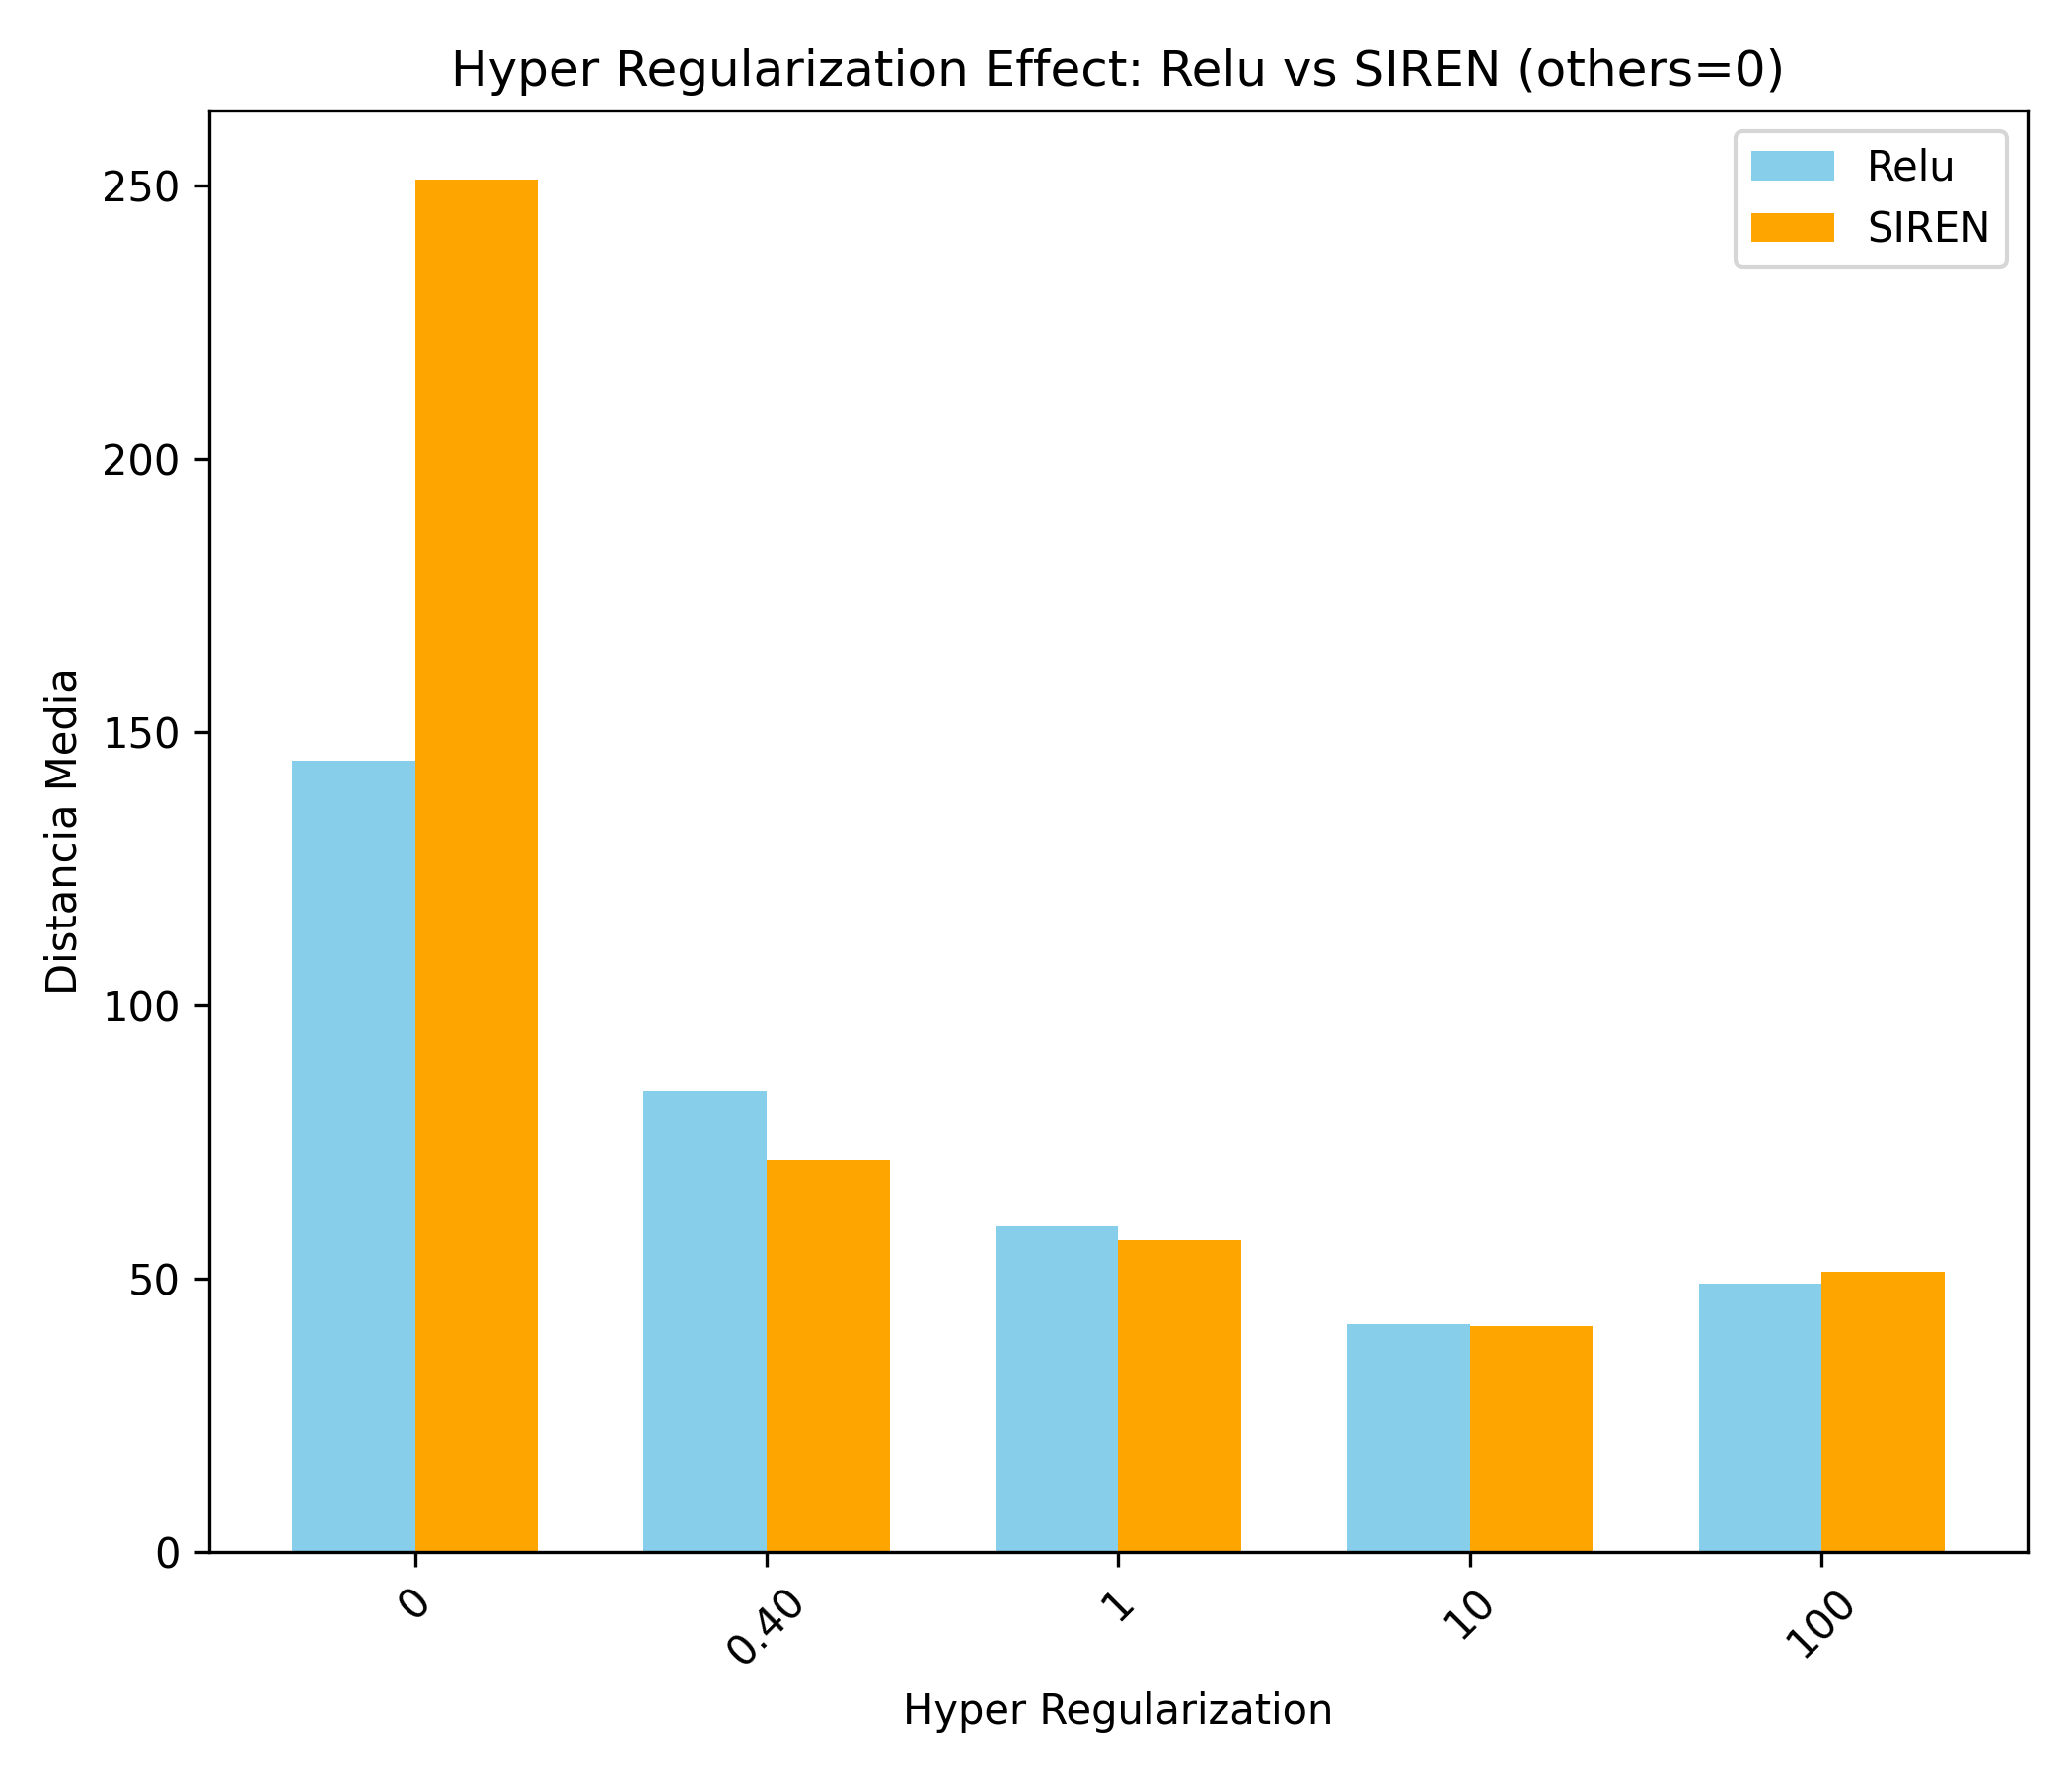
\includegraphics[width=\textwidth]{imaxes/reg_examples/barplot_hyper_reg_comparison_MLP_vs_SIREN_FIRE.png}
        \caption{Comparación de regularización hiperelástica en FIRE}
        \label{fig:barplot_hyper_reg_comparison_MLP_vs_SIREN_FIRE}
    \end{subfigure}\hfill
    \begin{subfigure}[b]{0.48\textwidth}
        \centering
        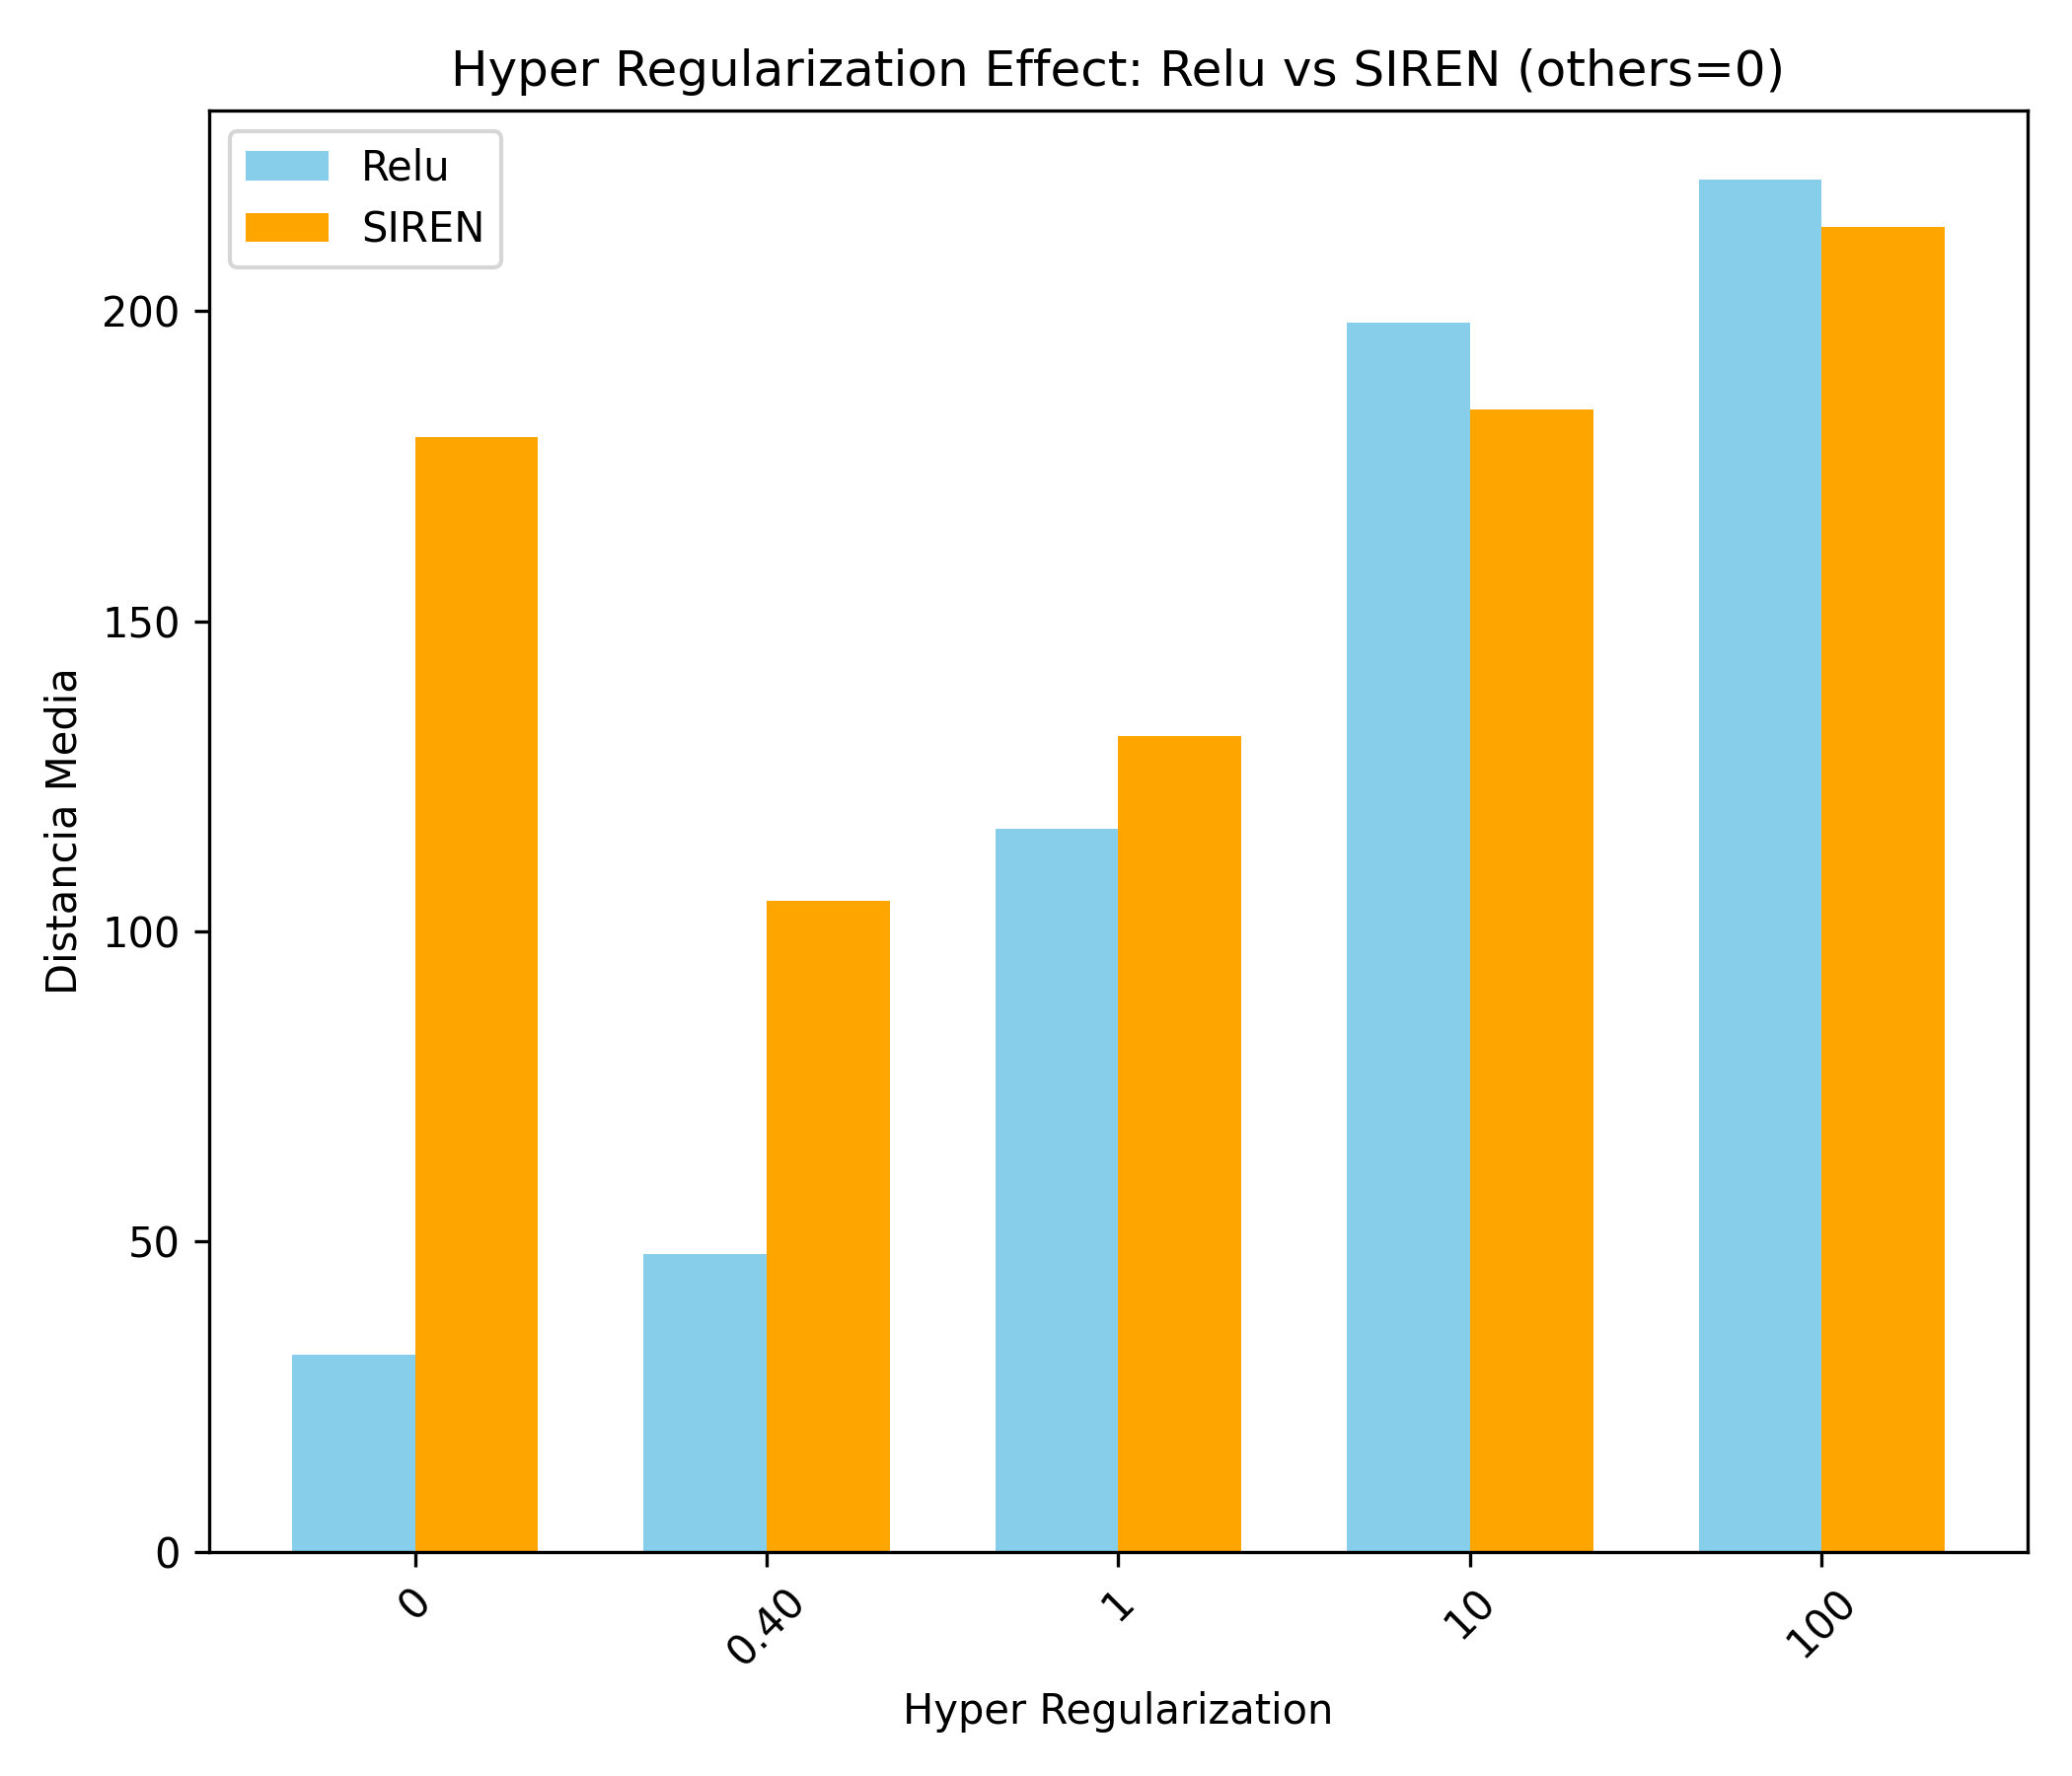
\includegraphics[width=\textwidth]{imaxes/reg_examples/barplot_hyper_reg_comparison_MLP_vs_SIREN_RFMID.png}
        \caption{Comparación de regularización hiperelástica en RFMID}
        \label{fig:barplot_hyper_reg_comparison_MLP_vs_SIREN_RFMID}
    \end{subfigure}
    \caption{Comparación del impacto de la regularización hiperelástica sobre los datasets FIRE y RFMID para modelos ReLU y SIREN}
    \label{fig:barplot_hyper_reg_comparison}
\end{figure}

\subsection{Discusión}
\label{subsec:Discusion-regularization}

Los resultados muestran que la regularización tiene un impacto significativo en el rendimiento de la red. Tanto la ausencia de regularización como la regularización excesiva resultan en rendimiento deficiente.
En la figura \ref{fig:regularization_examples} se pueden observar ejemplos de registros con ambos problemas.

\begin{figure}[tbp]
    \centering
    \begin{subfigure}[b]{0.45\textwidth}
        \centering
        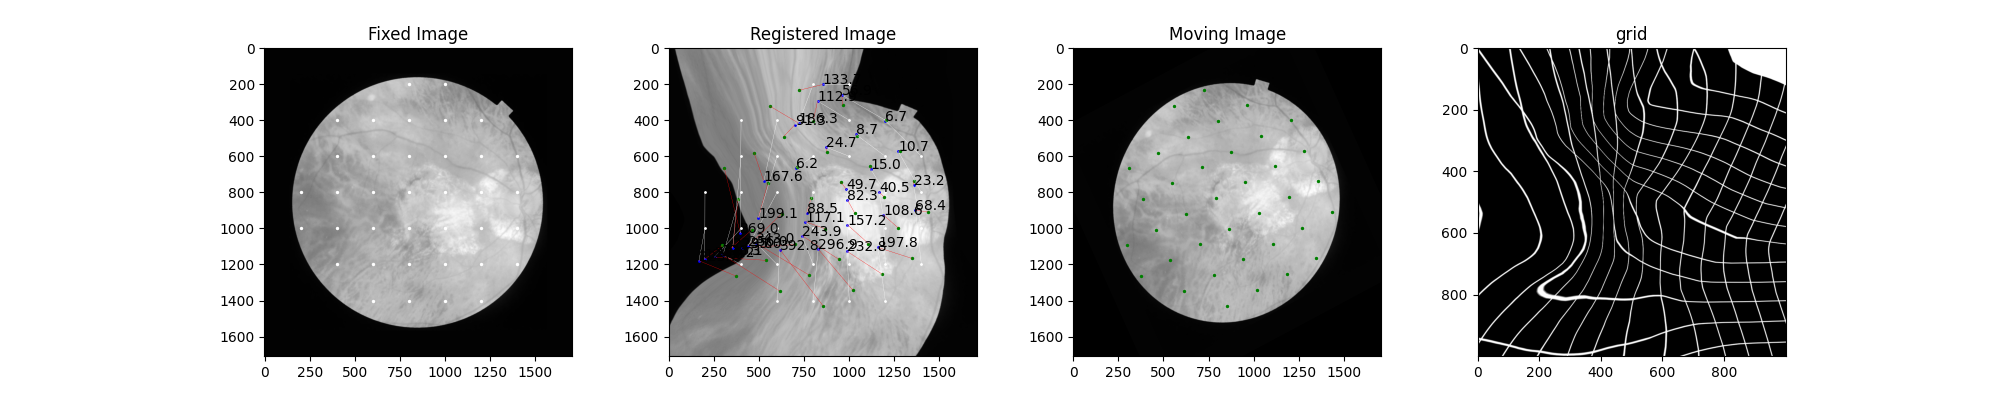
\includegraphics[width=\textwidth]{imaxes/reg_examples/no_reg_example.png}
        \caption{Ejemplo de registro con cero regularización, lo que provoca pliegues}
        \label{fig:no_reg_example}
    \end{subfigure}\hfill
    \begin{subfigure}[b]{0.45\textwidth}
        \centering
        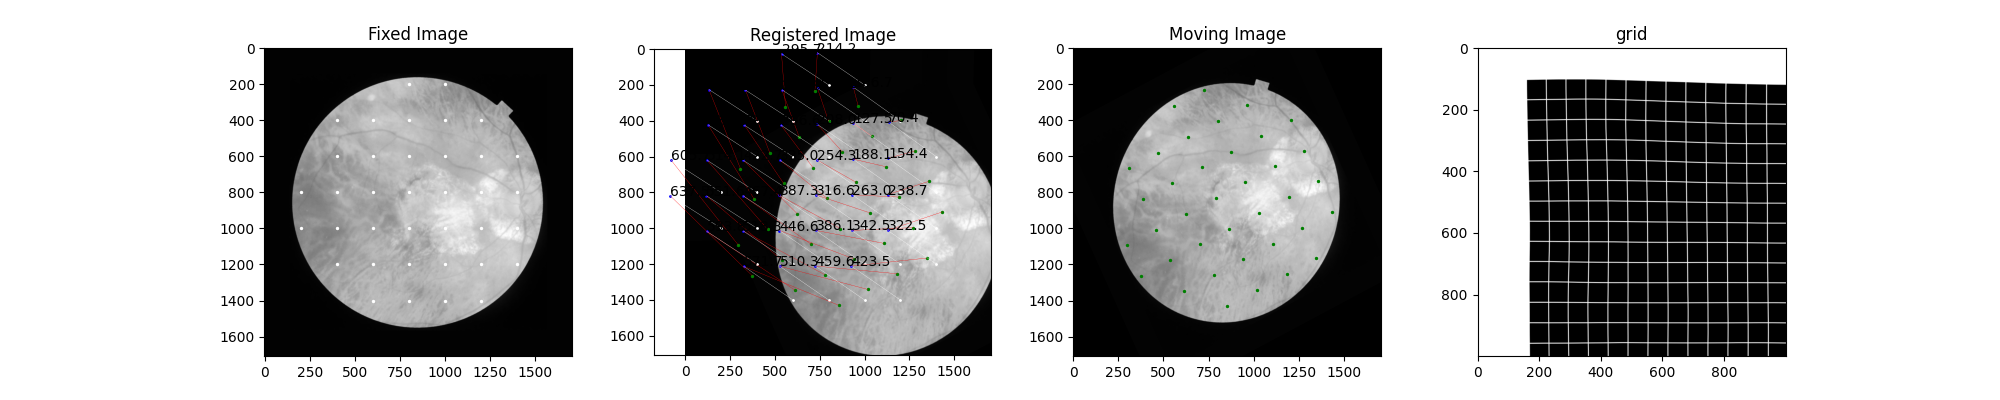
\includegraphics[width=\textwidth]{imaxes/reg_examples/too_much_reg_example.png}
        \caption{Ejemplo de registro con regularización excesiva, lo que evita que la red aprenda la transformación adecuada}
        \label{fig:too_much_reg_example}
    \end{subfigure}
    \caption{Ejemplos de registro con ausencia y exceso de regularización}
    \label{fig:regularization_examples}
\end{figure}

En los resultados se observa que Relu sigue dando mejores resultados que SIREN en el dataset RFMID, mientras que en el dataset FIRE ambos parecen tener un rendimiento similar.

La regularización óptima depende del tipo de registro que se está realizando. Los registros de transformaciones lineales (RFMID) se benefician de poca o ninguna regularización, mientras que los registros de transformaciones no lineales (FIRE) y con poca superposición se benefician de regularizaciones más elevadas.
Esto sugiere que la regularización es más relevante donde la red tiene que aprender transformaciones más complejas, ya que evita que caiga en mínimos locales no deseados.% \label{subsec:Conclusions-regularization}

En base a los resultados, se concluye que la regularización es un componente indispensable para el registro de retinas con redes implícitas. Su valor óptimo no es universal, sino que depende directamente de la complejidad de la transformación a aprender. Para deformaciones sencillas y lineales como las de RFMiD, una regularización mínima es suficiente, pero para los desafíos presentes en FIRE, con una mayor no linealidad, un término de regularización robusto es crucial para guiar la red hacia soluciones físicamente plausibles y evitar el sobreajuste. Se confirma también que los modelos SIREN, por su mayor capacidad para representar detalles de alta frecuencia, son más sensibles a la regularización y requieren valores generalmente más altos que los modelos ReLU para prevenir artefactos. La elección del coeficiente de regularización debe considerarse una decisión fundamental, adaptada tanto a la naturaleza del problema de registro como a la arquitectura de la red empleada.

\section{Tamaño de lote}
\label{sec:Tamaño de lote}

\subsection{Planteamiento}
\label{subsec:Planteamento-batchsize}

A lo largo de los experimentos realizados, el análisis cualitativo reveló que el tamaño de lote es uno de los parámetros que más impacto tiene en el rendimiento de la red.

De ahora en adelante dividimos el conjunto de datos de RFMID en varios subconjuntos según la dificultad de la transformación, como detallado en la sección \ref{subsec:Avaliación Cuantitativa}.

De esta forma podemos comparar el rendimiento de la red en diferentes subconjuntos de imágenes, y determinar si el rendimiento de la red es consistente entre ellos.

En los experimentos con el dataset FIRE, se decidió limitarse a la categoría S, ya que es la que mayor número de ejemplos tiene y tiene un mayor grado de superposición entre las imágenes, lo que facilita la tarea de registro.
Además, ya que la red sí que es capaz de registrar correctamente las imágenes de los subconjuntos más sencillos, utilizaremos la métrica de FIRE para medir el porcentaje de imágenes registradas correctamente.

\subsection{Resultados}
\label{subsec:Resultados-batchsize}

En las figuras \ref{fig:batch_size_comparison_relu_rfmid} y \ref{fig:batch_size_comparison_siren_rfmid} se pueden observar los resultados de la experimentación con el dataset RFMID a distintas dificultades y con distintos tamaños de lote.

\begin{figure}[tbp]
    \centering
    \begin{subfigure}[b]{0.5\textwidth}
        \centering
        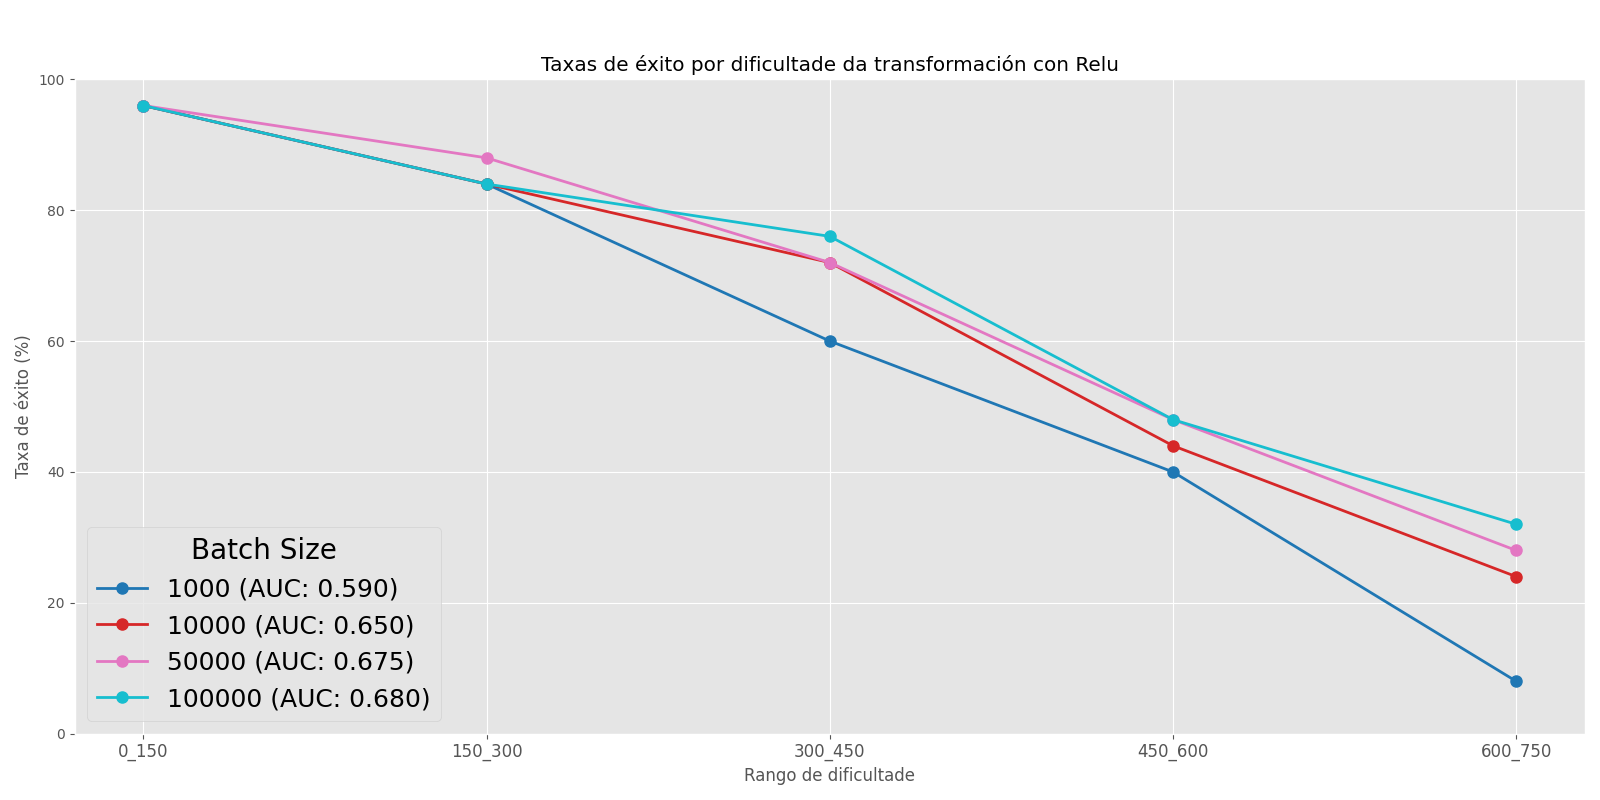
\includegraphics[width=\textwidth]{imaxes/batchsize/experiment_plot_RFMID_bs_relu.png}
        \caption{Función de activación ReLU}
        \label{fig:batch_size_comparison_relu_rfmid}
    \end{subfigure}\hfill
    \begin{subfigure}[b]{0.5\textwidth}
        \centering
        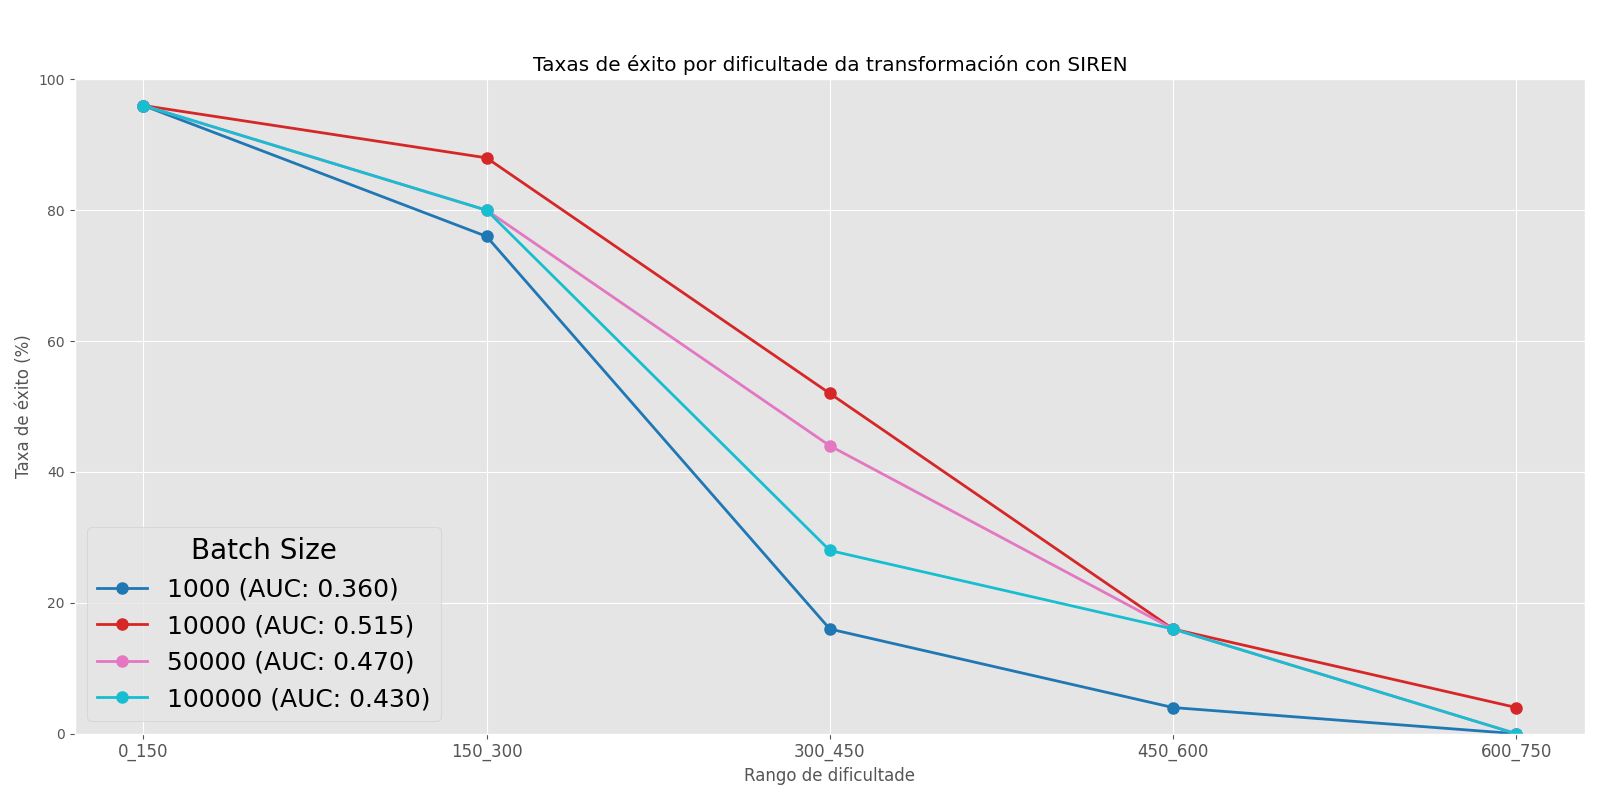
\includegraphics[width=\textwidth]{imaxes/batchsize/experiment_plot_RFMID_bs_siren.png}
        \caption{Función de activación SIREN}
        \label{fig:batch_size_comparison_siren_rfmid}
    \end{subfigure}
    \caption{Comparación del rendimiento de la red con diferentes tamaños de lote sobre imágenes del dataset RFMID, mostrando el porcentaje de registros exitosos para cada umbral de error.}
    \label{fig:batch_size_comparisons_rfmid}
\end{figure}

Con esta nueva división del dataset, también se realizó la evaluación por el método de evaluación de FIRE, que se puede ver en las figuras \ref{fig:FIRERFMID_relu} y \ref{fig:FIRERFMID_SIREN}.

\begin{figure}[tbp]
    \centering
    \begin{subfigure}[b]{0.5\textwidth}
        \centering
        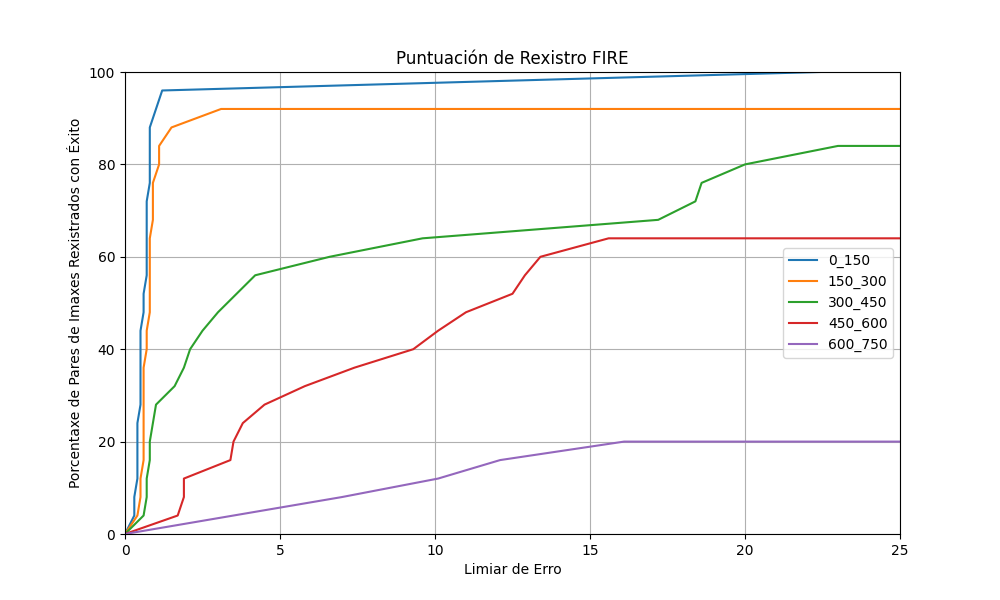
\includegraphics[width=\textwidth]{imaxes/FIRE_scores/fire_registration_scores_RFMID_MLP.png}
        \caption{Métrica FIRE con la función de activación ReLU}
        \label{fig:FIRERFMID_relu}
    \end{subfigure}\hfill
    \begin{subfigure}[b]{0.5\textwidth}
        \centering
        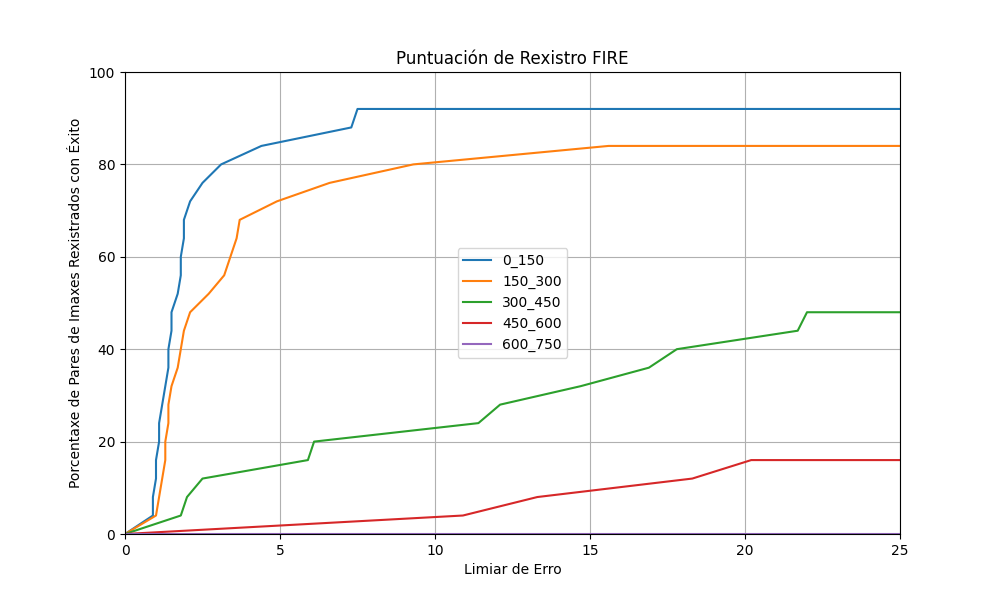
\includegraphics[width=\textwidth]{imaxes/FIRE_scores/fire_registration_scores_RMIFD_SIREN.png}
        \caption{Métrica FIRE con la función de activación SIREN}
        \label{fig:FIRERFMID_SIREN}
    \end{subfigure}
    \caption{Comparación del rendimiento de la red con diferentes tamaños de lote sobre imágenes del dataset FIRE}
    \label{fig:FIRERFMID_scores}
\end{figure}

En las figuras \ref{fig:batch_size_comparison_relu} y \ref{fig:batch_size_comparison_siren} se muestran los resultados de la experimentación con el dataset FIRE.

\begin{figure}[tbp]
    \centering
    \begin{subfigure}[b]{0.5\textwidth}
        \centering
        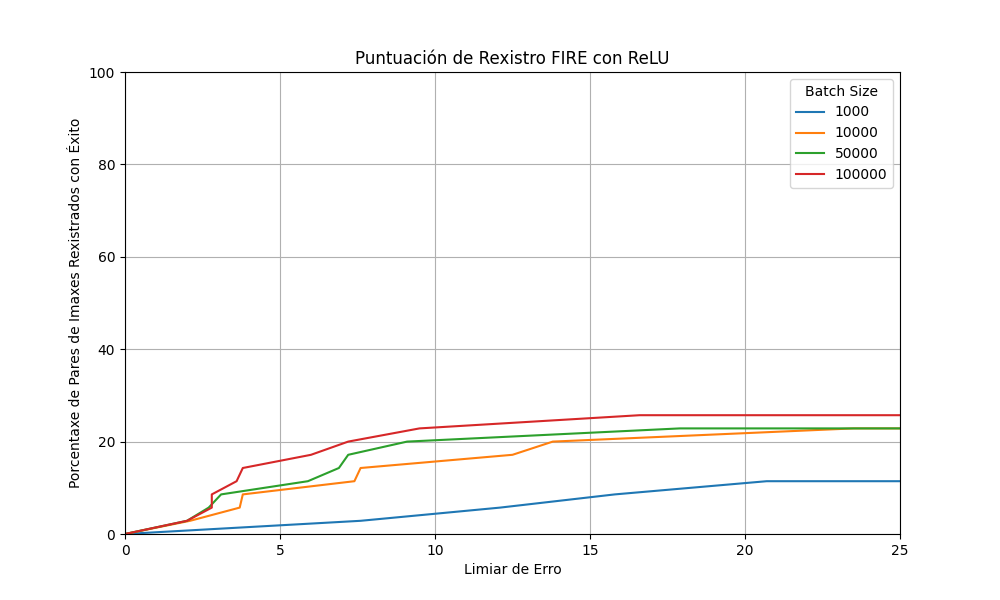
\includegraphics[width=\textwidth]{imaxes/batchsize/fire_registration_scores_bs_relu_S.png}
        \caption{Función de activación ReLU}
        \label{fig:batch_size_comparison_relu}
    \end{subfigure}\hfill
    \begin{subfigure}[b]{0.5\textwidth}
        \centering
        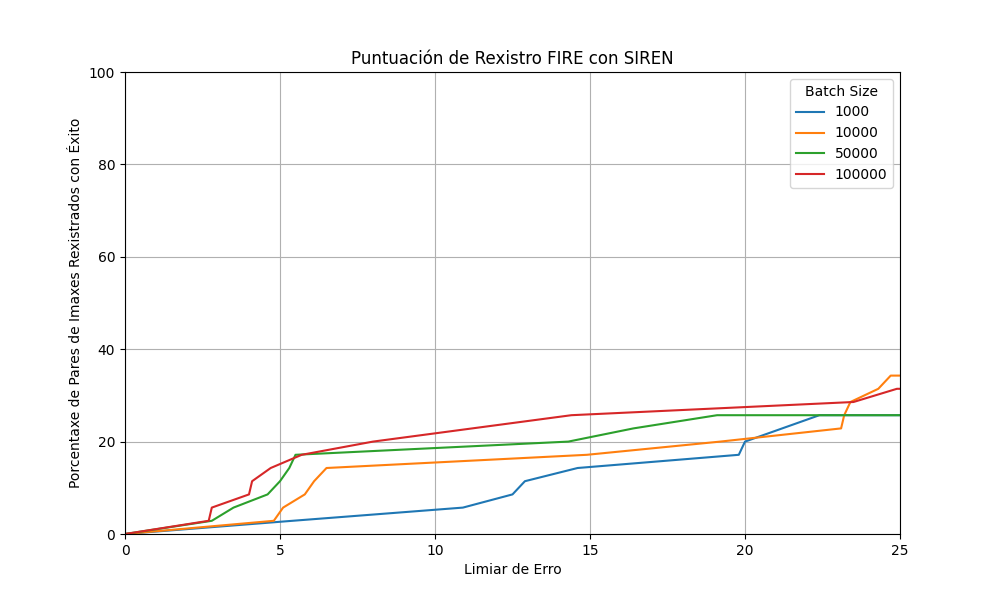
\includegraphics[width=\textwidth]{imaxes/batchsize/fire_registration_scores_bs_siren_S.png}
        \caption{Función de activación SIREN}
        \label{fig:batch_size_comparison_siren}
    \end{subfigure}
    \caption{Comparación del rendimiento de la red con diferentes tamaños de lote sobre imágenes de la categoría S del dataset FIRE}
    \label{fig:batch_size_comparisons_fire}
\end{figure}

\subsection{Discusión}
\label{subsec:Discusion-batchsize}

Se observa que las redes con la función de activación ReLU tienden a tener un rendimiento mucho mejor que las con la función de activación SIREN. Esto puede explicarse ya que las deformaciones artificiales que se aplican en las imágenes del dataset RFMID son lineales, y la función de activación ReLU es adecuada para este tipo de transformaciones.

También parece que el tamaño de lote es relevante, especialmente el cambio entre 1000 y 10000, mientras que valores mayores (50000, 100000) no parecen tener tanto impacto, aunque sí un mayor coste computacional.

Mientras que la red es capaz de registrar correctamente consistentemente las imágenes del subconjunto más sencillo (0-150, 150-300), el rendimiento decae notablemente para transformaciones más complejas (300+).
Esto es más notable cuando se utiliza la función de activación SIREN, que tiene dificultades incluso con transformaciones de complejidad media, mientras que con ReLU decae de forma lineal.

\subsection{Conclusiones}\label{subsec:Conclusions-batchsize}

El principal factor limitador del rendimiento de la red es el tamaño y complejidad de las transformaciones que intenta aprender.
Un tamaño de lote mayor parece ayudar, pero no es suficiente para registrar correctamente las imágenes con transformaciones más difíciles.

\section{Estrategias de muestreo}
\label{sec:Estratexias de mostraxe}

Originalmente IDIR utiliza una estrategia de muestreo aleatorio para seleccionar los puntos que se pasan a la red en cada iteración.
Mientras que esta estrategia parece suficiente para el registro de pulmones, en el caso de las imágenes de retina esto no tiene por qué ser así.
Esto se debe a que las imágenes de retina contienen secciones con mucha más información que otras, frente a los CTs de pulmones donde la señal es más uniforme.
Por ejemplo, las secciones que contienen vasos sanguíneos o el disco óptico probablemente tengan mayor cantidad de información relevante para la tarea de registro, frente a otras secciones como el fondo de la retina.
Además, las retinografías tienen desplazamientos mucho mayores y menor superposición entre cada pareja, por lo que la red tiene que aprender transformaciones más complejas.

\subsection{Planteamiento}
\label{subsec:Plantexamento-sampling}

Se plantearon nuevas estrategias de muestreo, explicadas en detalle en el apartado \ref{subsec:Metodoloxías Desenvoltas}, con las cuales se pretende mejorar el rendimiento de la red al proporcionarle más información relevante para la tarea de registro.
Las estrategias de muestreo comparadas son las siguientes:
\begin{itemize}
    \item Muestreo aleatorio: Selección aleatoria de puntos de la imagen.
    \item Muestreo uniforme: Selección de puntos uniformemente espaciados en la imagen. Especialmente relevante cuando se usan tamaños de lote pequeños, ya que permite garantizar que se muestran puntos de toda la imagen.
    \item Muestreo inteligente: Selección de puntos basándose en la información del gradiente de la imagen, priorizando las áreas con mayor variación.
    \item Muestreo ponderado: Punto intermedio entre el muestreo aleatorio y el inteligente, donde se seleccionan puntos aleatoriamente pero con mayor probabilidad en las áreas de mayor interés.
\end{itemize}

\subsection{Resultados}
\label{subsec:Resultados-sampling}

Los resultados de las diferentes estrategias de muestreo sobre el dataset RFMID se presentan en la figura \ref{fig:sampling_types_comparisons}.

\begin{figure}[tbp]
    \centering
    \begin{subfigure}[b]{0.48\textwidth}
        \centering
        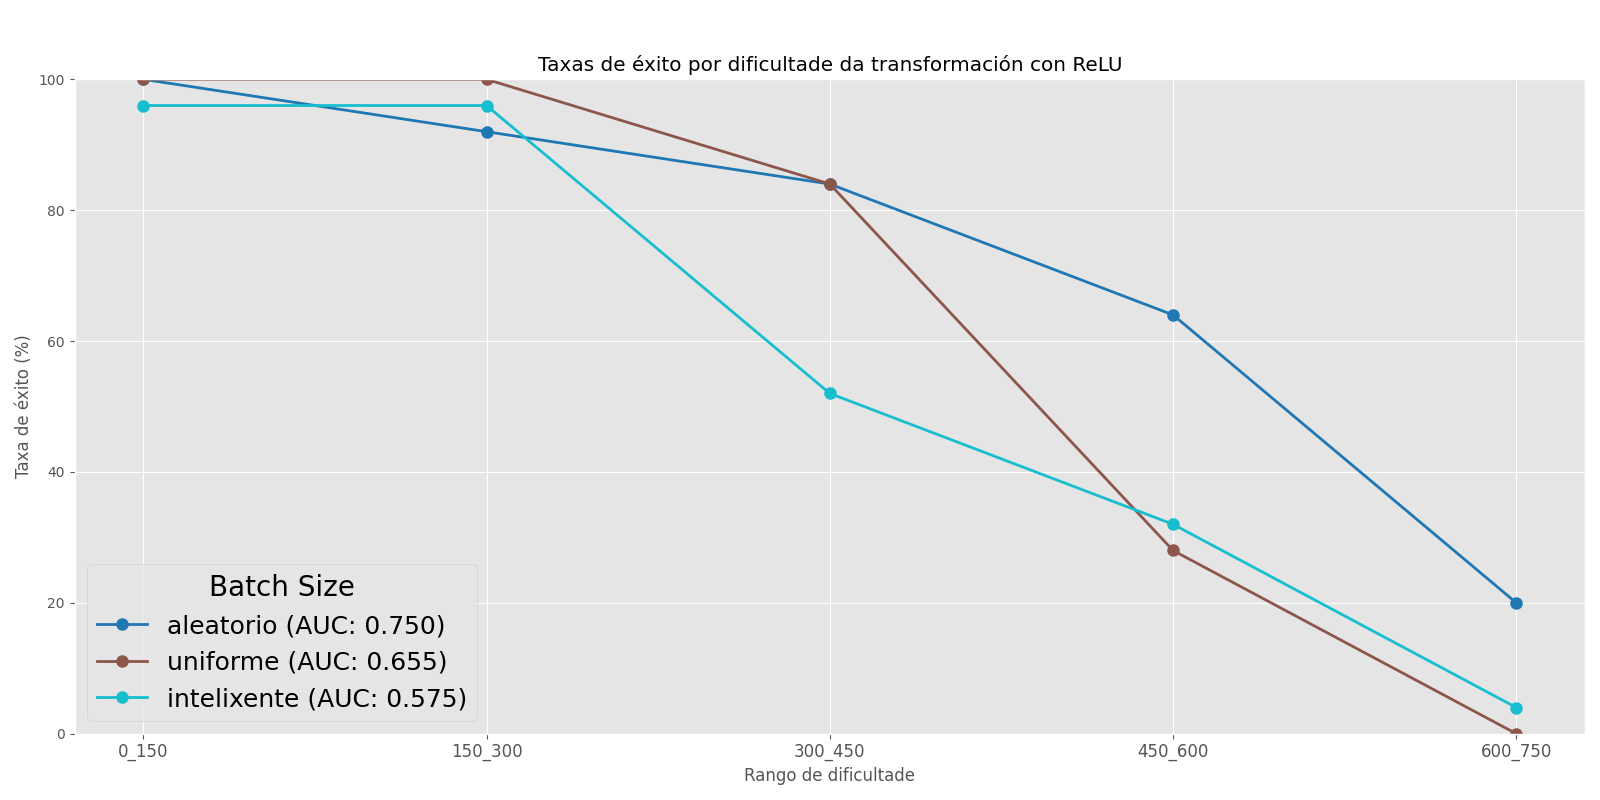
\includegraphics[width=\textwidth]{imaxes/muestraje/experiment_plot_RFMID_st_relu.png}
        \caption{Función de activación ReLU}
        \label{fig:sampling_types_relu}
    \end{subfigure}\hfill
    \begin{subfigure}[b]{0.48\textwidth}
        \centering
        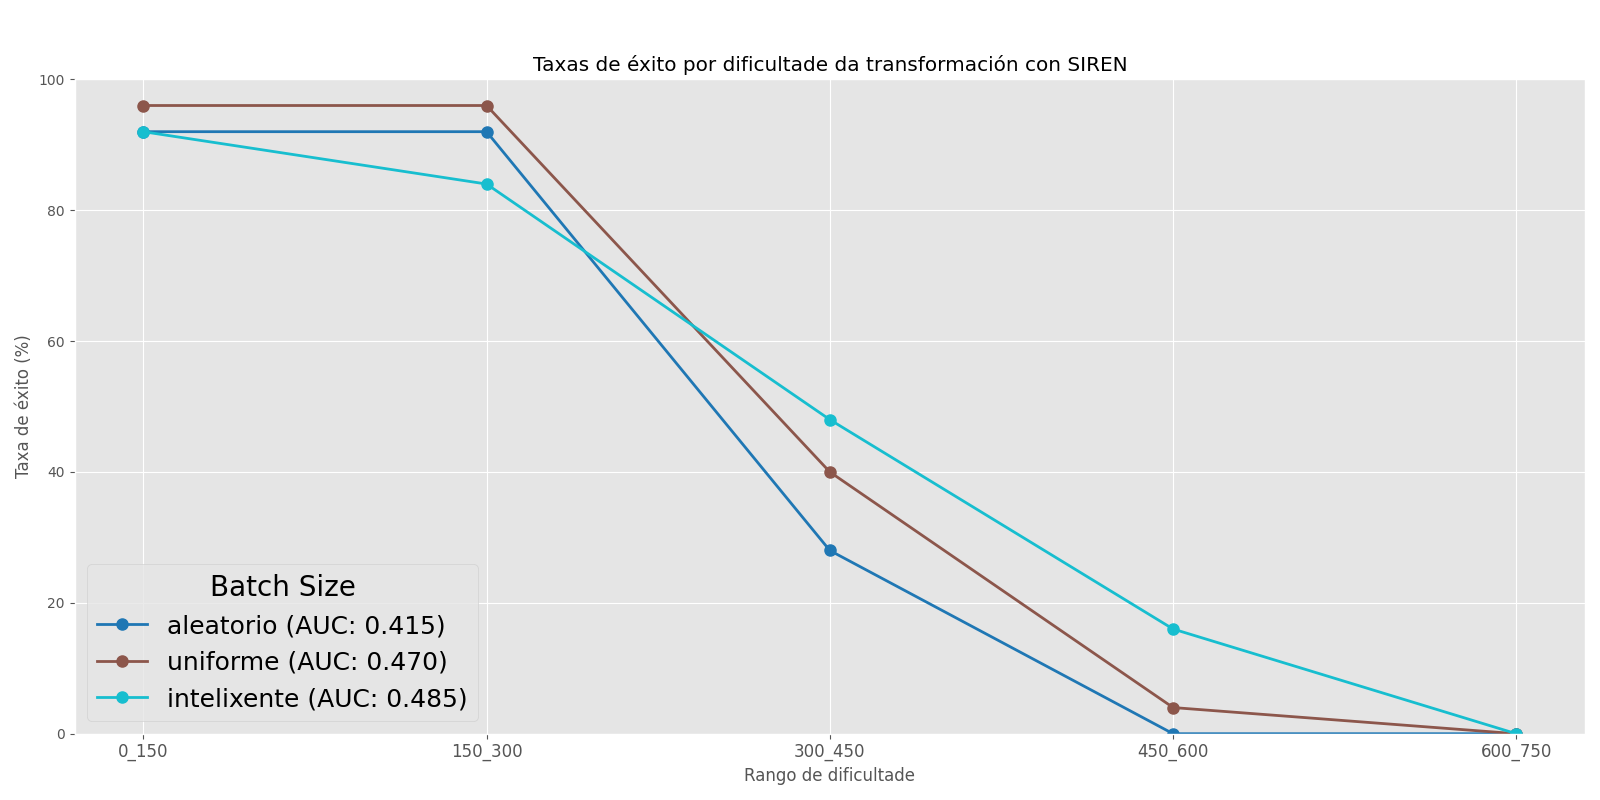
\includegraphics[width=\textwidth]{imaxes/muestraje/experiment_plot_RFMID_st_SIREN.png}
        \caption{Función de activación SIREN}
        \label{fig:sampling_types_siren}
    \end{subfigure}
    \caption{Comparación de las diferentes estrategias de muestreo sobre imágenes del dataset RFMID}
    \label{fig:sampling_types_comparisons}
\end{figure}

\subsection{Discusión}
\label{subsec:Discusion-sampling}

La hipótesis de la estrategia de muestreo inteligente no parece ser adecuada, con resultados similares a la estrategia aleatoria. 
Lo mismo ocurre con la estrategia uniforme.

Igual que en experimentos anteriores, la función de activación ReLU parece dar mejores resultados que SIREN con RFMID, especialmente con mayores dificultades de transformación.

\subsection{Conclusiones}
\label{subsec:Conclusions-sampling}
Se concluye que, en contra de la hipótesis inicial, las estrategias de muestreo implementadas, como la ponderada por el contenido de la imagen, no aportan una mejora significativa en el rendimiento del registro en comparación con el muestreo aleatorio estándar. Esto sugiere que la información relevante para la deformación está lo suficientemente bien distribuida como para que un muestreo aleatorio sea capaz de capturar los puntos necesarios para la convergencia, siempre que el tamaño de lote sea adecuado.

\section{Inicialización}
\label{sec:Inicialización}

\subsection{Planteamiento}
\label{subsec:Planteamento-initialization}

Es posible que la inicialización de la red sea un factor clave, y que ciertos desplazamientos iniciales provoquen que la red sea incapaz de aprender la transformación correcta, o que le cueste mucho más aprenderla.

Para validar esta hipótesis se implementó una lotería de inicialización, donde se utiliza la pérdida en la época 0 para determinar la inicialización de la red más beneficiosa sobre la que seguir entrenando.

\begin{figure}[tbp]
    \centering
    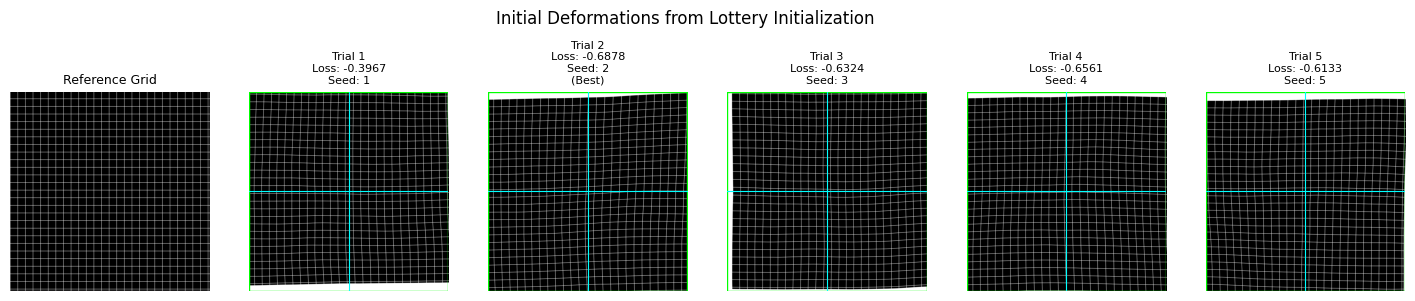
\includegraphics[width=0.8\textwidth]{imaxes/lottery/initial_deformations_combinedMLP.png}
    \caption{Ejemplos de las diferentes inicializaciones con la función de activación RELU}
    \label{fig:lottery_initial_deformations_combinedMLP}
\end{figure}

\begin{figure}[tbp]
    \centering
    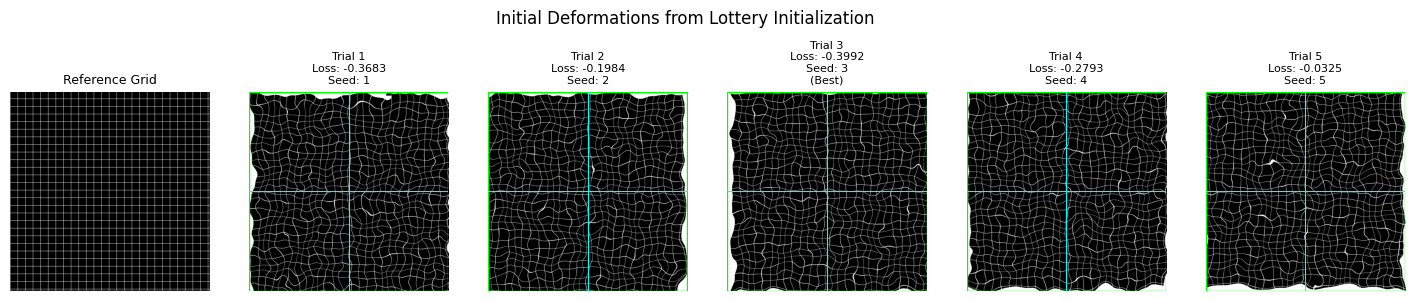
\includegraphics[width=0.8\textwidth]{imaxes/lottery/initial_deformations_combinedSIREN.png}
    \caption{Ejemplos de las diferentes inicializaciones con la función de activación SIREN}
    \label{fig:lottery_initial_deformations_combinedSIREN}
\end{figure}

\subsection{Resultados}
\label{subsec:Resultados-initialization}

En la figura \ref{fig:lottery} se muestran los resultados de diferentes valores de la lotería de inicialización.

\begin{figure}[tbp]
    \centering
    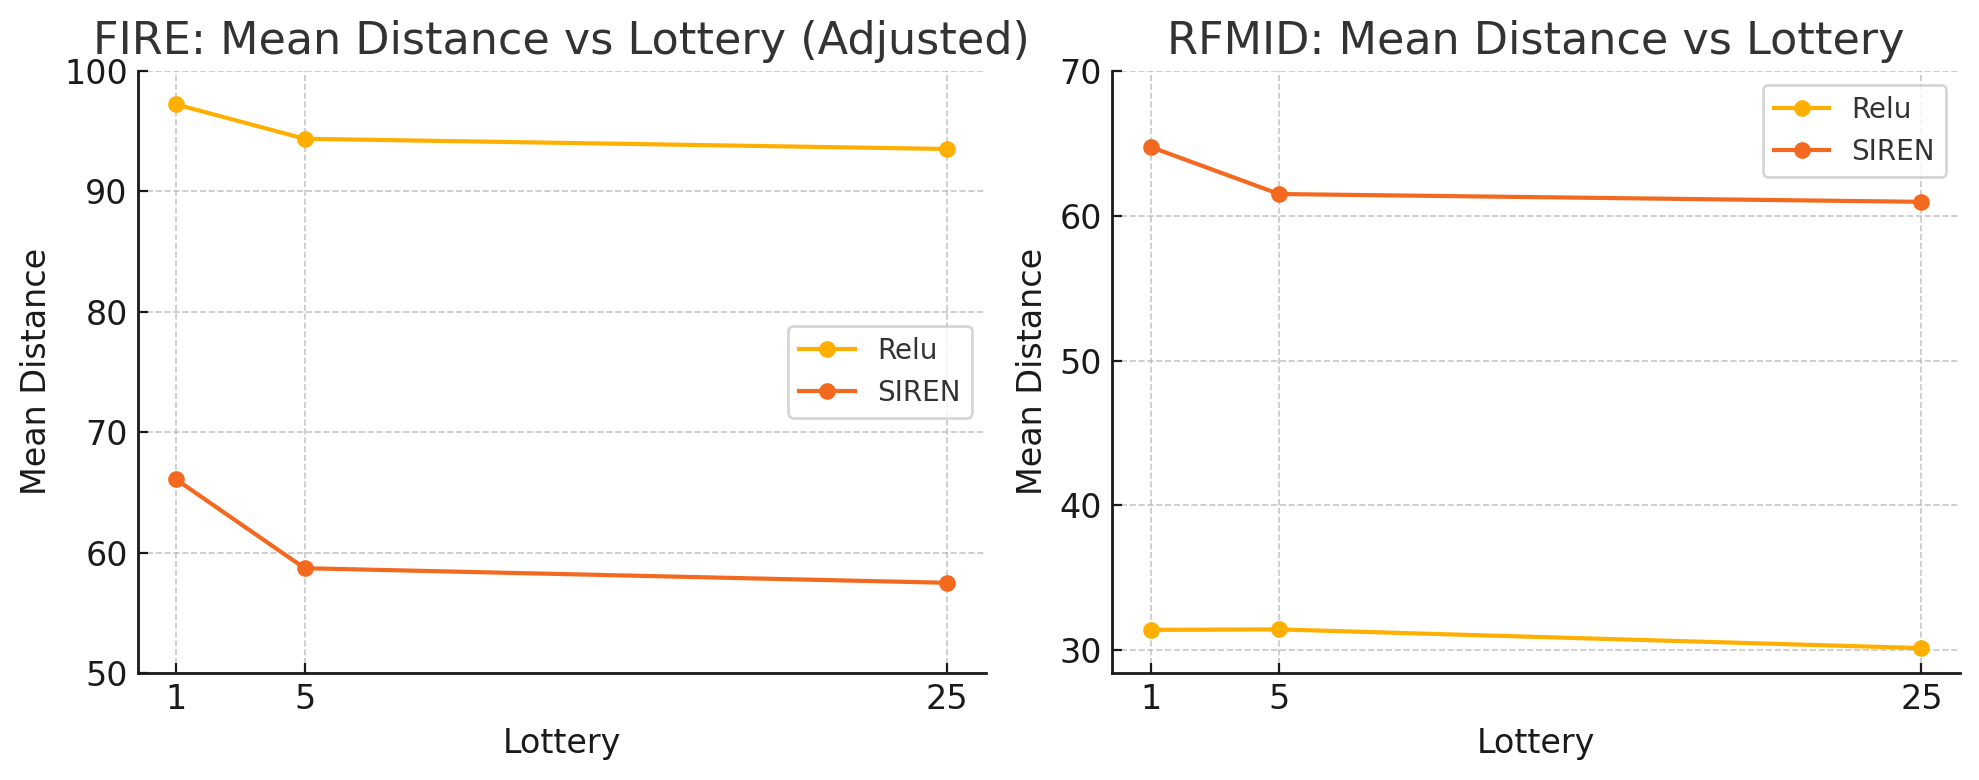
\includegraphics[width=0.8\textwidth]{imaxes/lottery/lotery.png}
    \caption{Resultados de la lotería de inicialización}
    \label{fig:lottery}
\end{figure}

\subsection{Discusión}
\label{subsec:Discusion-initialization}

La inicialización estándar de SIREN propuesta por Sitzmann et al. \cite{sitzmann2020implicitneuralrepresentationsperiodic} fue diseñada para tareas de reconstrucción de imágenes, y no necesariamente para regresión de campos de deformación.
Esto puede provocar que el proceso de optimización dedique mucho tiempo a contrarrestar una mala inicialización.

\subsection{Conclusiones}
\label{subsec:Conclusions-initialization}

Se observa que la lotería de inicialización sí que provoca mejoras en el rendimiento de la red, aunque no muy significativas, y no se beneficia particularmente de utilizar más de 5 inicializaciones.
Es posible que fuera mejor esperar hasta una iteración algo más avanzada para determinar la inicialización, ya que en la época 0 no hay ninguna seguridad de que no sea un mínimo local, pero esto también implicaría un mayor coste computacional.

Una posible mejora a la lotería de inicialización sería utilizar un número mayor de épocas antes de determinar la inicialización ganadora, ya que la pérdida inicial no es necesariamente representativa del rendimiento final de la red.
De la misma forma, sería interesante comparar diferentes estrategias de inicialización, como la inicialización gaussiana o la inicialización uniforme, para determinar si alguna de ellas proporciona una ventaja significativa sobre la inicialización estándar de SIREN.

\section{Ajuste dinámico del tamaño de lote}
\label{sec:Dynamic tamaño de lote}

\subsection{Planteamiento}
\label{subsec:Planteamento-phases}

Se teoriza que la red puede beneficiarse de dividir el proceso de registro en diferentes fases, donde inicialmente se utiliza un tamaño de lote reducido para aprender la transformación global, y posteriormente se aumenta el tamaño de lote para aprender las transformaciones locales.
Para esto utilizaremos la estrategia de muestreo uniforme, que permite asegurar que se cubre toda la imagen con la misma densidad, lo que es más importante con tamaños de lote pequeños. El learning rate se modifica de forma proporcional para mantener la relación entre este y el tamaño de lote.

\subsection{Resultados}
\label{subsec:Resultados-phases}

Los resultados de utilizar diferentes números de fases se pueden observar en la figura \ref{fig:nphases}.
\begin{figure}[tbp]
    \centering
    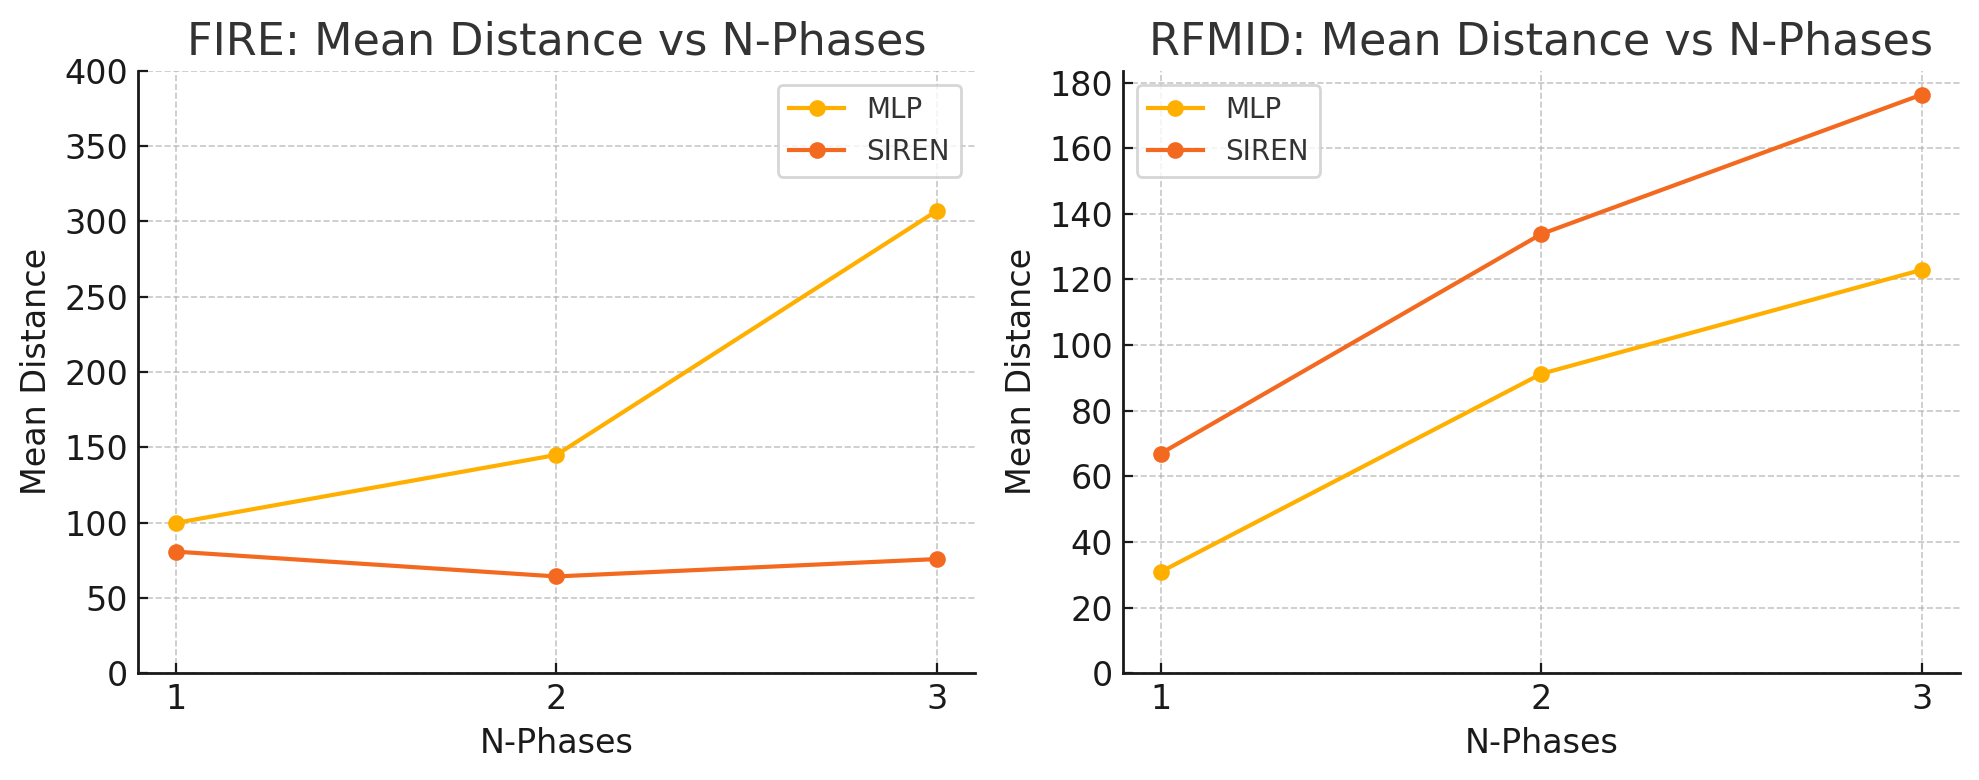
\includegraphics[width=0.8\textwidth]{imaxes/lottery/nphases.png}
    \caption{Resultados de usar distinto número de fases}
    \label{fig:nphases}
\end{figure}

\subsection{Discusión}\label{subsec:Discusion-phases}

Los resultados presentados en la figura \ref{fig:nphases} muestran una tendencia clara y contraria a la hipótesis inicial, ya que el rendimiento de la red empeora progresivamente a medida que se incrementa el número de fases. La estrategia de comenzar con un tamaño de lote pequeño para aprender la transformación global antes de refinar los detalles con un tamaño de lote mayor resulta ser contraproducente.

Una posible explicación es que la idea de que un lote pequeño favorece el aprendizaje global es incorrecta en este contexto. Un tamaño de lote reducido ofrece una estimación muy ruidosa y poco representativa, lo que puede llevar el entrenamiento por un camino inestable e impedir que la red converja hacia una buena solución global en la fase inicial. En cambio, un tamaño de lote grande y constante, como se validó en la sección \ref{sec:Tamaño de lote}, proporciona desde el principio información suficiente tanto a nivel global como local, permitiendo que la red aprenda ambas transformaciones simultáneamente de forma más estable y eficaz.

Por lo tanto, la estrategia de dividir el entrenamiento en fases no solo no aporta beneficios, sino que resulta perjudicial al introducir inestabilidad en las etapas cruciales del aprendizaje. Este experimento refuerza la conclusión de que un tamaño de lote grande es fundamental para el éxito del registro con esta metodología.

\subsection{Conclusiones}
\label{subsec:Conclusions-phases}

Se concluye que la estrategia de ajuste dinámico del tamaño de lote es ineficaz y perjudicial para esta tarea. La inestabilidad introducida en las fases iniciales del entrenamiento anula cualquier posible beneficio teórico de aprender las transformaciones por etapas. La red demuestra ser más robusta y eficaz cuando se entrena con un tamaño de lote grande y constante desde el principio, confirmando que este enfoque es superior para aprender simultáneamente las características globales y locales de la deformación.

% \FloatBarrier

\section{Comparativa y resumen de resultados}
\label{sec:Comparativa e resumo}

Tras la realización de los experimentos descritos anteriormente, se pueden extraer las siguientes conclusiones:

\subsection{Rendimiento por dataset}
\label{subsec:Rendemento por dataset}

\textbf{Dataset FIRE:} El rendimiento en el dataset FIRE, que contiene imágenes reales de retina, es significativamente más bajo que en el dataset RFMID. La categoría P resulta imposible de registrar debido al bajo grado de superposición (<75\%). Las categorías S y A muestran tasas de éxito alrededor del 20\%, siendo la categoría S ligeramente superior.

\textbf{Dataset RFMID:} El rendimiento en el dataset RFMID es considerablemente mejor, especialmente para transformaciones de baja complejidad (norma de Frobenius 0-150), donde se alcanza un éxito del casi 100\%. El rendimiento decae progresivamente con la complejidad de la transformación.

\subsection{Comparación de funciones de activación}
\label{subsec:Comparación de funcións de activación}

Los resultados muestran una clara diferenciación entre las funciones de activación según el tipo de dataset:

\textbf{ReLU:} Muestra un rendimiento superior en el dataset RFMID, debido a su capacidad natural para aprender transformaciones lineales.

\textbf{SIREN:} Aunque teóricamente más adecuada para aprender transformaciones complejas, tiene dificultades para representarlas adecuadamente. Tiende a transformaciones locales y poco realistas y si no se regulariza adecuadamente, converge a mínimos locales no deseados.

\subsection{Impacto de los parámetros principales}
\label{subsec:Impacto dos parámetros principais}

\textbf{Función de pérdida:} Las métricas basadas en características estructurales (NCC, SSIM) son superiores para imágenes reales con variabilidad de iluminación (FIRE), mientras que las métricas basadas en píxeles (L1, MSE) son más efectivas para imágenes sin variabilidad (RFMID).

\textbf{Regularización:} La regularización hiperelástica es la más relevante para evitar deformaciones no realistas. El valor óptimo depende del par de imágenes concreto a registrar. SIREN requiere valores más altos que ReLU ya que tiene una mayor tendencia al sobreajuste.

\textbf{Tamaño de lote:} Constituye uno de los parámetros más críticos. Valores mayores (10000-50000) proporcionan mejores resultados que tamaños pequeños (1000), aunque el beneficio decrece para valores muy altos (>50000).

\textbf{Resolución:} No se observan beneficios significativos por encima de 1000×1000 píxeles, sugiriendo que la información relevante para el registro ya está capturada en resoluciones moderadas.

\subsection{Limitaciones identificadas}
\label{subsec:Limitacións identificadas}

\textbf{Complejidad de las transformaciones:} El factor limitador principal es la complejidad de las transformaciones. Tanto ReLU como SIREN muestran dificultades con las transformaciones de alta complejidad, independientemente de la optimización de parámetros.

\textbf{Superposición de imágenes:} La baja superposición entre imágenes (categoría P de FIRE) dificulta enormemente el registro, sugiriendo que las redes implícitas requieren un mínimo de información compartida.

\textbf{Estrategias de muestreo:} Contrario a lo esperado, las estrategias inteligentes de muestreo (ponderadas por contenido) no muestran beneficios sobre el muestreo aleatorio, sugiriendo que la información relevante está distribuida de forma más uniforme de lo esperado.

\subsection{Conclusiones generales}
\label{subsec:Conclusións xerais}

La fase experimental de este trabajo, centrada en la adaptación y evaluación de un marco basado en representación neuronales implícitas para la tarea de registro de imágenes oftalmológicas, demuestra que las redes implícitas son aplicables al registro de imágenes de retina, pero con limitaciones importantes. El rendimiento depende críticamente de la complejidad de las transformaciones y del grado de superposición entre imágenes. Aunque los resultados son prometedores para casos de complejidad baja a moderada, el registro de imágenes con transformaciones complejas o baja superposición sigue siendo un desafío que requiere investigación adicional.

Si bien el rendimiento actual no es óptimo, las comparaciones con otras metodologías de registro del estado del arte deben tener en cuenta que la mayoría de ellas integran conocimiento específico del dominio frente al método aquí presentado, que funciona de forma general aprendiendo a partir de los píxeles. Esto sugiere futuras líneas de investigación que combinen las ventajas de las redes implícitas con conocimientos específicos del dominio, como la anatomía de la retina o las características de los vasos sanguíneos, para mejorar el rendimiento en registros complejos. El análisis de las limitaciones del modelo y exploración de diferentes estrategias proporcionan una base sólida para futuras investigaciones en el campo.
 \chapter{Conclusiones}
\label{chap:Conclusións}

\lettrine{E}{n} conclusión, el proyecto de investigación realizado consistió en la adaptación del framework IDIR para el registro de retinografías.
En especial valoramos el uso de la función de activación SIREN, propuesta como alternativa a la función ReLU para mejorar la representación de las deformaciones.

La alineación de retinografías es un problema relevante ya que es un proceso laborioso para los expertos, pero con mucha utilidad clínica.
La etapa inicial de la revisión del estado del arte reveló que ya existían varios trabajos previos que abordaban este problema, siendo los más exitosos los basados en métodos iterativos.
Actualmente los métodos de aprendizaje profundo son una alternativa prometedora que está ganando prominencia en el campo. Particularmente, el uso de representaciones implícitas para esta tarea es un enfoque innovador que ya fue aplicado en otros campos de la imagen médica con buenos resultados.

Para evaluar la efectividad del método propuesto, se escogieron dos conjuntos de datos de retinografías: FIRE, que permite la evaluación del método en imágenes reales, y RFMID, sobre el que se efectuaron transformaciones artificiales para simular diferentes escenarios de alineación.

Durante la fase de experimentación se exploraron diferentes combinaciones de hiperparámetros (pérdida, regularización, resolución...) y se introdujeron diferentes técnicas para intentar mejorar la convergencia del modelo, como diferentes esquemas de muestreo, inicialización, y técnicas de ajuste dinámico del tamaño de lote.

Algunas de las dificultades encontradas durante el desarrollo del proyecto fueron: la falta de documentación sobre el funcionamiento del código original, que dificultó su adaptación al nuevo dominio; el diseño del proceso de evaluación, en el cual fue complejo encontrar visualizaciones que permitiesen interpretar los resultados fácilmente; y el tiempo de cómputo que requerían algunos experimentos, que requirió la implementación de optimizaciones para facilitar la experimentación.

Los resultados obtenidos muestran que esta arquitectura no es la más adecuada para la tarea de registro de retinografías.

Sí se obtienen buenos resultados en el dataset RFMID, que se basa en imágenes con transformaciones lineales sintéticas, donde la función de activación ReLU tiende a obtener mejores resultados que SIREN, ya que está mejor preparada para representar las transformaciones lineales globales que se producen entre estas imágenes.
Se observa también que el tamaño de la transformación tiene un impacto significativo en el rendimiento, ya que las imágenes de mayor tamaño presentan un mayor error de registro.

En el dataset FIRE, que contiene imágenes reales, los resultados son peores que en el dataset RFMID, especialmente en las parejas de imágenes que presentan grandes deformaciones o bajo nivel de superposición.
La función de activación SIREN obtiene mejores resultados aquí, ya que es capaz de representar mejor las deformaciones no lineales y locales que se producen entre las imágenes.

Estas diferencias en el rendimiento destacan la importancia de la elección de la función de activación en función de la naturaleza específica de las transformaciones esperadas.
La fase de experimentación también reveló que la regularización es un factor fundamental, especialmente en la función de activación SIREN, donde la ausencia de regularización lleva a un sobreajuste significativo y a un rendimiento muy pobre.

Cabe destacar que el método presentado en este trabajo guía la optimización con tan solo la métrica de NCC, que depende únicamente de las intensidades de los píxeles, y que en registros con mucho desplazamiento o deformaciones complejas la topografía de función de pérdida será poco convexa y con múltiples mínimos locales, lo que dificulta la convergencia del modelo.
Por el contrario, métodos como REMPE \cite{rempe} que obtienen resultados mucho mejores (registra con éxito la totalidad de la categoría S de FIRE) hacen uso de información adicional que les permite establecer correspondencias globales entre las imágenes.

Una observación relevante es la diferencia entre el rendimiento entre el conjunto de datos sintético (RFMID) y el conjunto de datos real (FIRE). Esta brecha demuestra la dificultad de aplicar modelos entrenados en datos sintéticos a imágenes reales.

Tener una función de pérdida que dependa solo de las intensidades de los píxeles, como la NCC, limita la capacidad del modelo para capturar correspondencias globales y estabilidad de optimización, especialmente en imágenes con grandes deformaciones o variaciones de apariencia.
La inestabilidad de optimización es otro desafío importante, ya que es sensible a la inicialización y propensa a mínimos locales deficientes.

Este trabajo muestra que los modelos \gls{INR} puramente basados en imágenes carecen de los mecanismos de correspondencia global y estabilidad de optimización necesarias para aproximar grandes deformaciones y variaciones de apariencia presentes en muchas de las imágenes clínicas de retina.

Todos estos hallazgos responden a los objetivos propuestos en el inicio del proyecto, donde adaptamos el framework IDIR para el registro de retinografías, exploramos la función de activación SIREN y evaluamos el rendimiento del modelo en diferentes condiciones.
 \chapter{Trabajo futuro}
\label{chap:Traballo futuro}

\lettrine{E}{xisten} varias líneas de trabajo futuro que se pueden seguir para mejorar el sistema actual.
Los resultados obtenidos en este trabajo, aunque demuestran la viabilidad de adaptar el framework IDIR para el alineamiento de imágenes oftalmológicas 2D, también revelan limitaciones a la hora de alcanzar la precisión y robustez deseables.
Las siguientes líneas de trabajo futuro se consideran prometedoras para superar estos desafíos y avanzar en el campo:

\section{Arquitecturas alternativas}
\label{sec:Arquitecturas alternativas}

Una línea relevante de trabajo futuro es la exploración de arquitecturas alternativas.
Mientras que los perceptrones multicapa (MLPs) son considerados aproximadores universales \cite{HORNIK1989359} (son capaces de aproximar cualquier función continua dada una cantidad suficiente de neuronas), es posible que la arquitectura utilizada de 3 capas con 256 neuronas por capa no sea lo suficientemente grande para capturar las complejidades de las transformaciones entre las retinografías.

Una opción sería aumentar el número de capas o neuronas por capa. Otra sería implementar el uso de codificación posicional, que parece ser útil para la tarea de registro \cite{mueller2022instant}.

Otra idea muy interesante es el uso de restricciones de consistencia cíclicas, propuestas por Van Harten et al. en el contexto de registro de imágenes médicas \cite{van_Harten_2024}. Consiste en entrenar dos redes a la vez que estiman las transformaciones directas e inversas (una de la fija a la móvil y otra de la móvil a la fija), haciendo que estas se regularicen mutuamente y estabilizando la optimización.
Una ventaja de este enfoque es que produce una métrica de certidumbre al comparar las transformaciones estimadas, lo cual es muy útil en aplicaciones clínicas.

También podría ser interesante explorar el uso de meta-aprendizaje, donde se aprende una inicialización de pesos óptima a partir de un conjunto de datos \cite{learnedinit}, o condicionar por geometría, donde se incorpora conocimiento anatómico previo para simplificar la complejidad de la deformación \cite{harten2023deformable}.

\section{Invertibilidad}
\label{sec:Invertibilidade}

Una dirección interesante para el trabajo futuro es la exploración de métodos que garanticen la invertibilidad de las transformaciones aprendidas por la red.
La red IDIR actual no garantiza la invertibilidad de las transformaciones aprendidas, lo que significa que no es posible aplicar la transformación inversa de manera fiable.

Gracias a los términos de regularización utilizados durante el entrenamiento son pocos los casos en los que el determinante Jacobiano es negativo (lo que indicaría que la transformación no es invertible).

Aproximaciones como la de i-RevNet \cite{jacobsen2018irevnetdeepinvertiblenetworks} o aquellos basados en campos vectoriales de velocidad \cite{sun2024medicalimageregistrationneural} permiten garantizar la invertibilidad de las transformaciones aprendidas, lo que podría mejorar la precisión y la robustez del registro y funcionaría como un mecanismo de regulación implícita.

\section{Enfoque híbrido}
\label{sec:Enfoque híbrido}

Otra línea de trabajo futuro es la exploración de enfoques híbridos que combinen el registro basado en redes neuronales con técnicas tradicionales de registro.
Una posibilidad sería utilizar el registro tradicional para proporcionar un registro inicial y global robusto, que después podría ser refinado por una red neuronal.

Más concretamente, consistiría en utilizar un detector de puntos clave robusto como SuperPoint \cite{superpoint} para extraer características de las imágenes fija y móvil, y utilizar un algoritmo de emparejamiento de puntos clave como SuperGlue \cite{superglue} para obtener una transformación inicial entre las imágenes.
Posteriormente entrenaría el modelo INR para refinar esta transformación inicial, lo que es un problema de optimización más sencillo y que hace uso de las ventajas de ambos enfoques.

Este es el enfoque utilizado por métodos en el estado del arte como HybridRetina \cite{liu2024progressiveretinalimageregistration}.

Asimismo, se podrían explorar con más profundidad el preprocesado de las imágenes, ya que es inexistente en el método actual pero podría ser útil para mejorar la calidad de las imágenes y facilitar el registro.

 %%%%%%%%%%%%%%%%%%%%%%%%%%%%%%%%%%%%%%%%
 % Apéndices, glosarios e bibliografía  %
 %%%%%%%%%%%%%%%%%%%%%%%%%%%%%%%%%%%%%%%%

 \appendix
 \appendixpage
%  \chapter{Material adicional}
\label{chap:adicional}

\section{Anexo regularization}
\label{sec:Anexo regularization}

% \begin{table}[h]
%     \centering
%     \begin{minipage}[t]{0.45\linewidth}
%         \centering
%         \scriptsize
%         \setlength{\tabcolsep}{25pt}
%         \begin{tabular}{|c|c|}
%         \hline
%         Resolution & Mean Distance \\ \hline
%         100 & 254.22 \\ \hline
%         250 & 251.29 \\ \hline
%         750 & 250.62 \\ \hline
%         1250 & 250.59 \\ \hline
%         1708 & 249.72 \\ \hline
%         \end{tabular}
%         \caption{Distancias medias para o dataset FIRE ca función de activación Relu}
%         \label{tab:mlp_mean_distances_fire}
%     \end{minipage}
%     \hfill
%     \begin{minipage}[t]{0.45\linewidth}
%         \centering
%         \scriptsize
%         \setlength{\tabcolsep}{25pt}
%         \begin{tabular}{|c|c|}
%         \hline
%         Resolution & Mean Distance \\ \hline
%         100 & 266.43 \\ \hline
%         250 & 263.85 \\ \hline
%         750 & 263.19 \\ \hline
%         1250 & 258.56 \\ \hline
%         1708 & 258.06 \\ \hline
%         \end{tabular}
%         \caption{Distancias medias para o dataset FIRE ca función de activación SIREN}
%         \label{tab:siren_mean_distances_fire}
%     \end{minipage}
% \end{table}

% \begin{table}[h]
%     \centering
%     \begin{minipage}[t]{0.45\linewidth}
%         \centering
%         \scriptsize
%         \setlength{\tabcolsep}{25pt}
%         \begin{tabular}{|c|c|}
%         \hline
%         Resolution & Mean Distance \\ \hline
%         100 & 37.29 \\ \hline
%         250 & 36.18 \\ \hline
%         750 & 36.01 \\ \hline
%         1250 & 35.03 \\ \hline
%         1708 & 35.04 \\ \hline
%         \end{tabular}
%         \caption{Distancias medias para o dataset RFMID ca función de activación Relu}
%         \label{tab:mlp_mean_distances_rfmid}
%     \end{minipage}
%     \hfill
%     \begin{minipage}[t]{0.45\linewidth}
%         \centering
%         \scriptsize
%         \setlength{\tabcolsep}{25pt}
%         \begin{tabular}{|c|c|}
%         \hline
%         Resolution & Mean Distance \\ \hline
%         100 & 68.12 \\ \hline
%         250 & 73.42 \\ \hline
%         750 & 77.55 \\ \hline
%         1250 & 67.33 \\ \hline
%         1708 & 67.31 \\ \hline
%         \end{tabular}
%         \caption{Distancias medias para o dataset RMIFD ca función de activación SIREN}
%         \label{tab:siren_mean_distances_rfmid}
%     \end{minipage}
% \end{table}


\subsection{Figuras experimentos de regularización}
\label{subsec:figuras_experimentos_regularizacion}

\paragraph{Resultados}
\label{par:Resultados-reg2}

Os resultados da experimentación extendida da regularización, realizados sobre os datasets FIRE e RFMID, preséntanse nas figuras \ref{fig:gs_single_heatmaps}.

\begin{figure}[tbp]
    \centering
    \begin{subfigure}[b]{0.4\textwidth}
        \centering
        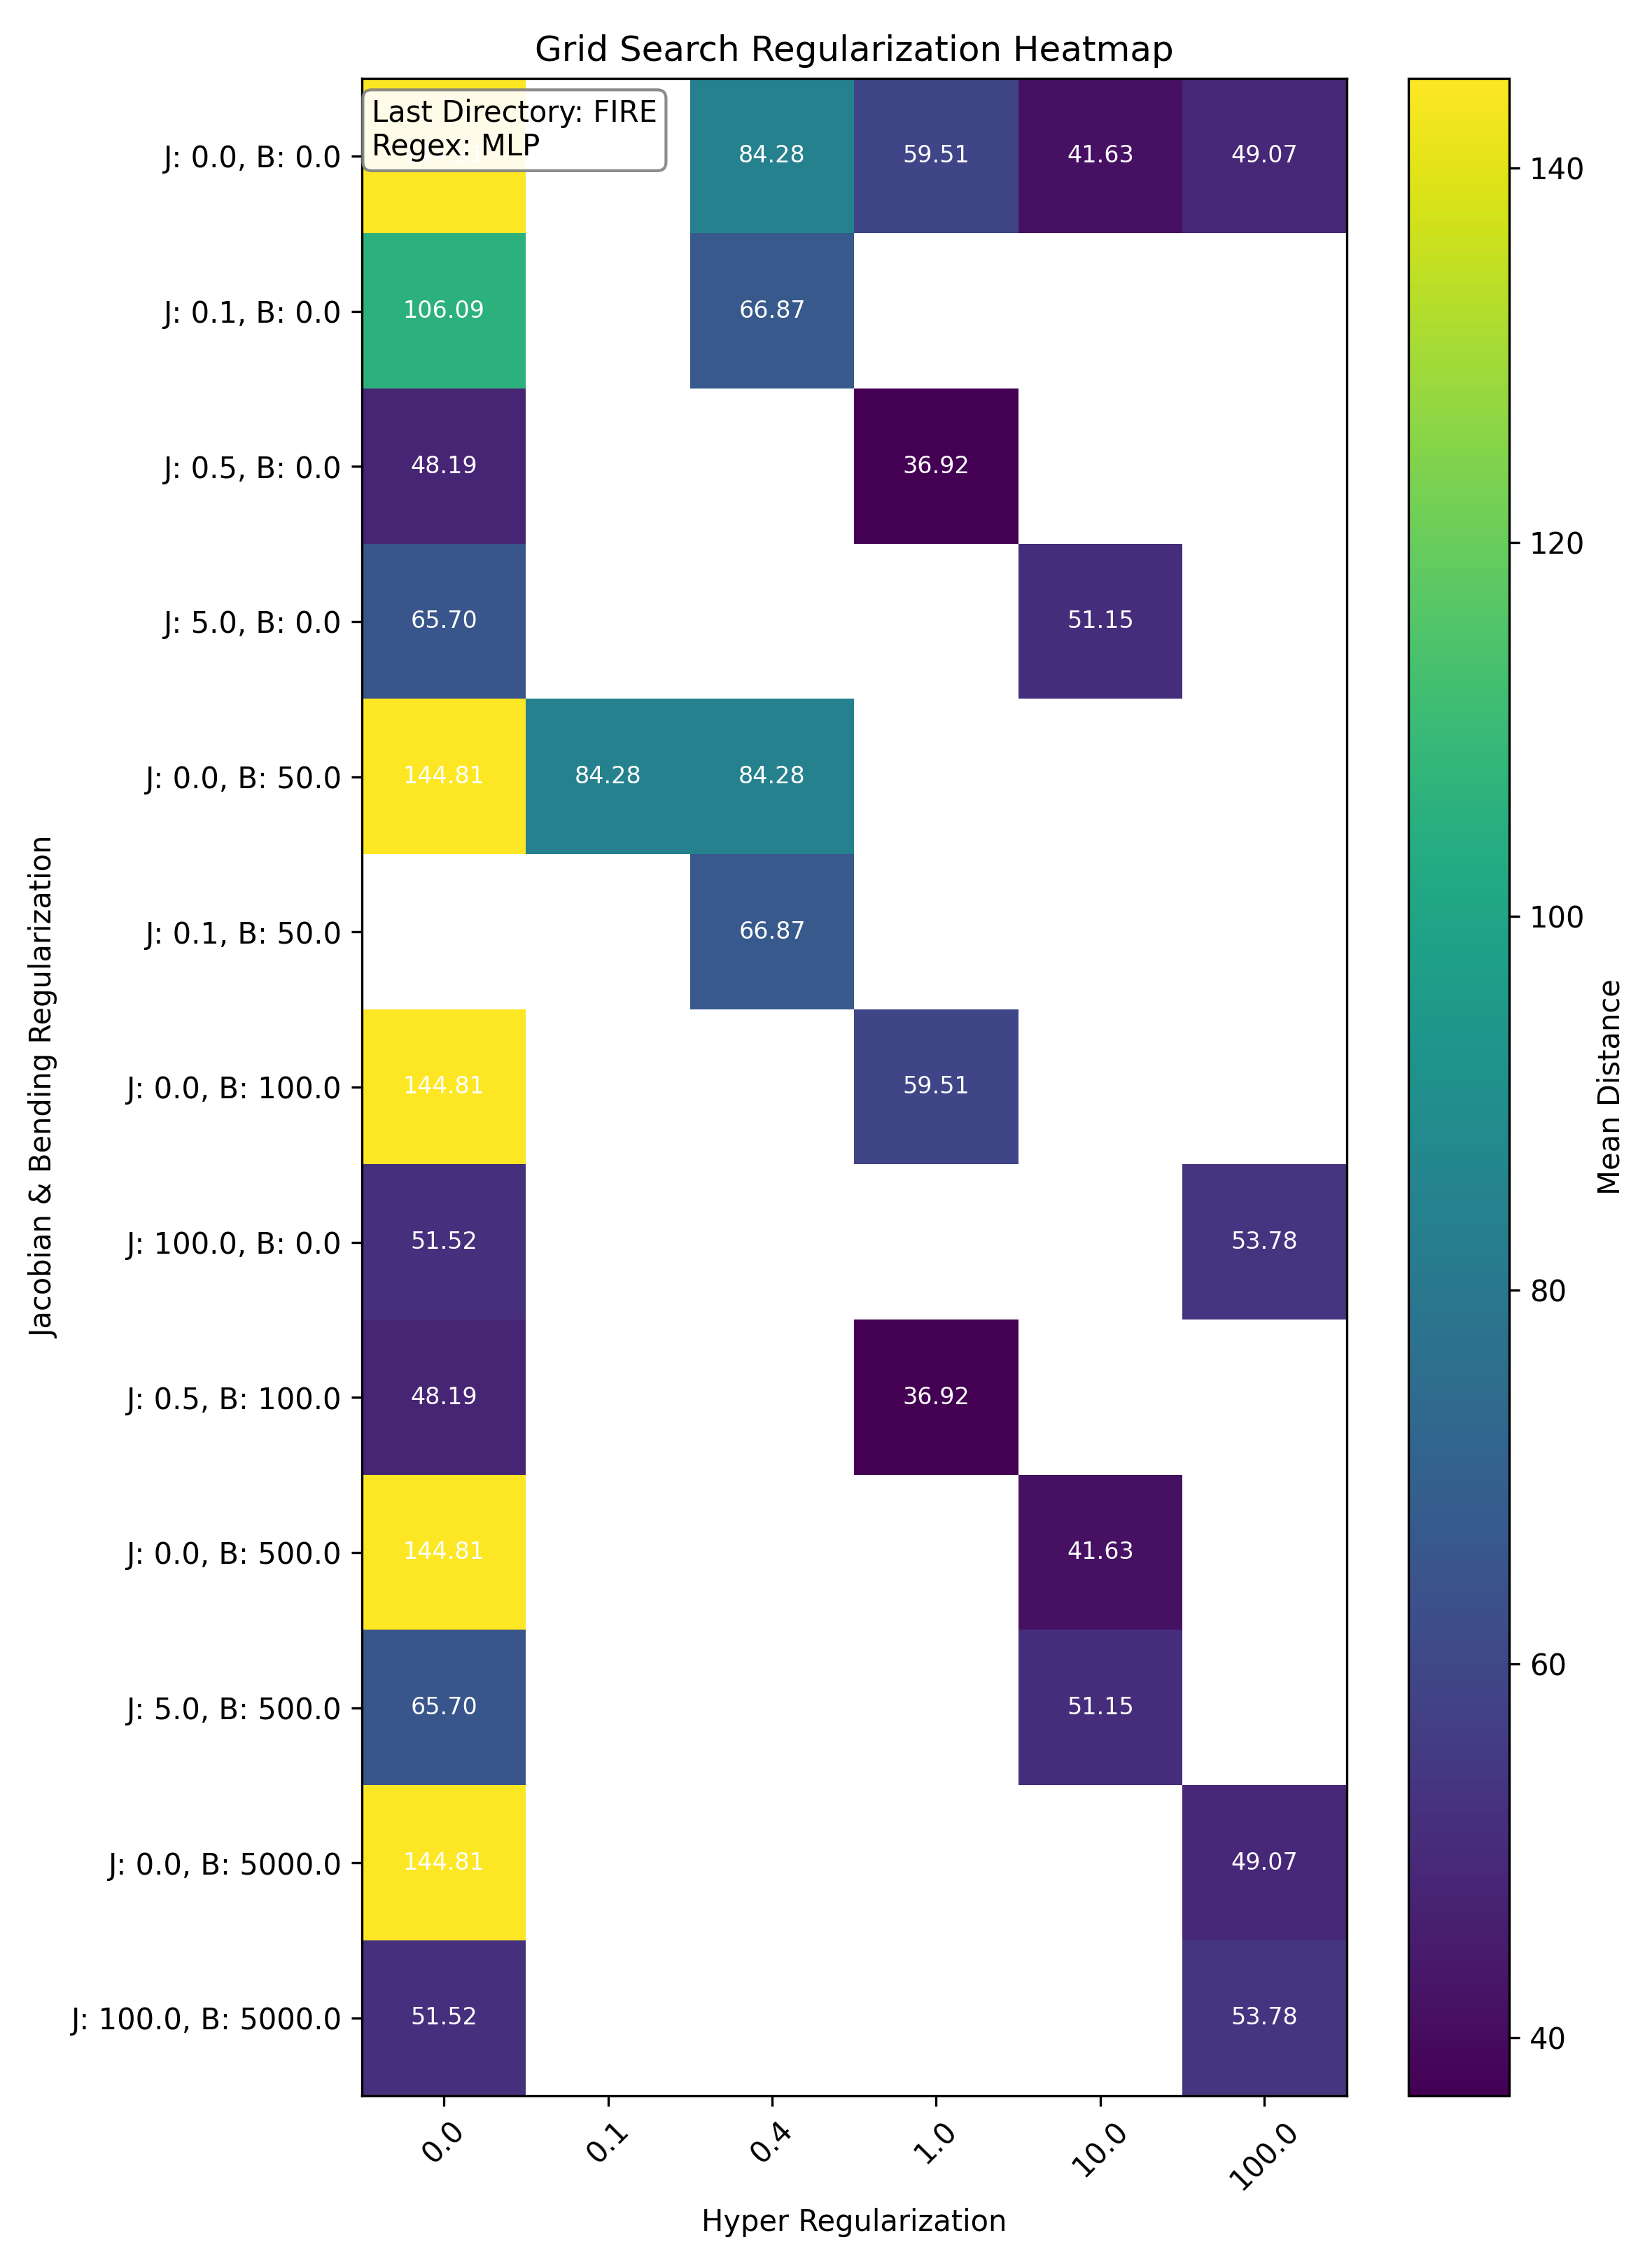
\includegraphics[width=\textwidth]{imaxes/grid_search_single_heatmap_FIRE_MLP.png}
        \caption{FIRE - Relu}
        \label{fig:gs_single_FIRE_MLP}
    \end{subfigure}\hfill
    \begin{subfigure}[b]{0.4\textwidth}
        \centering
        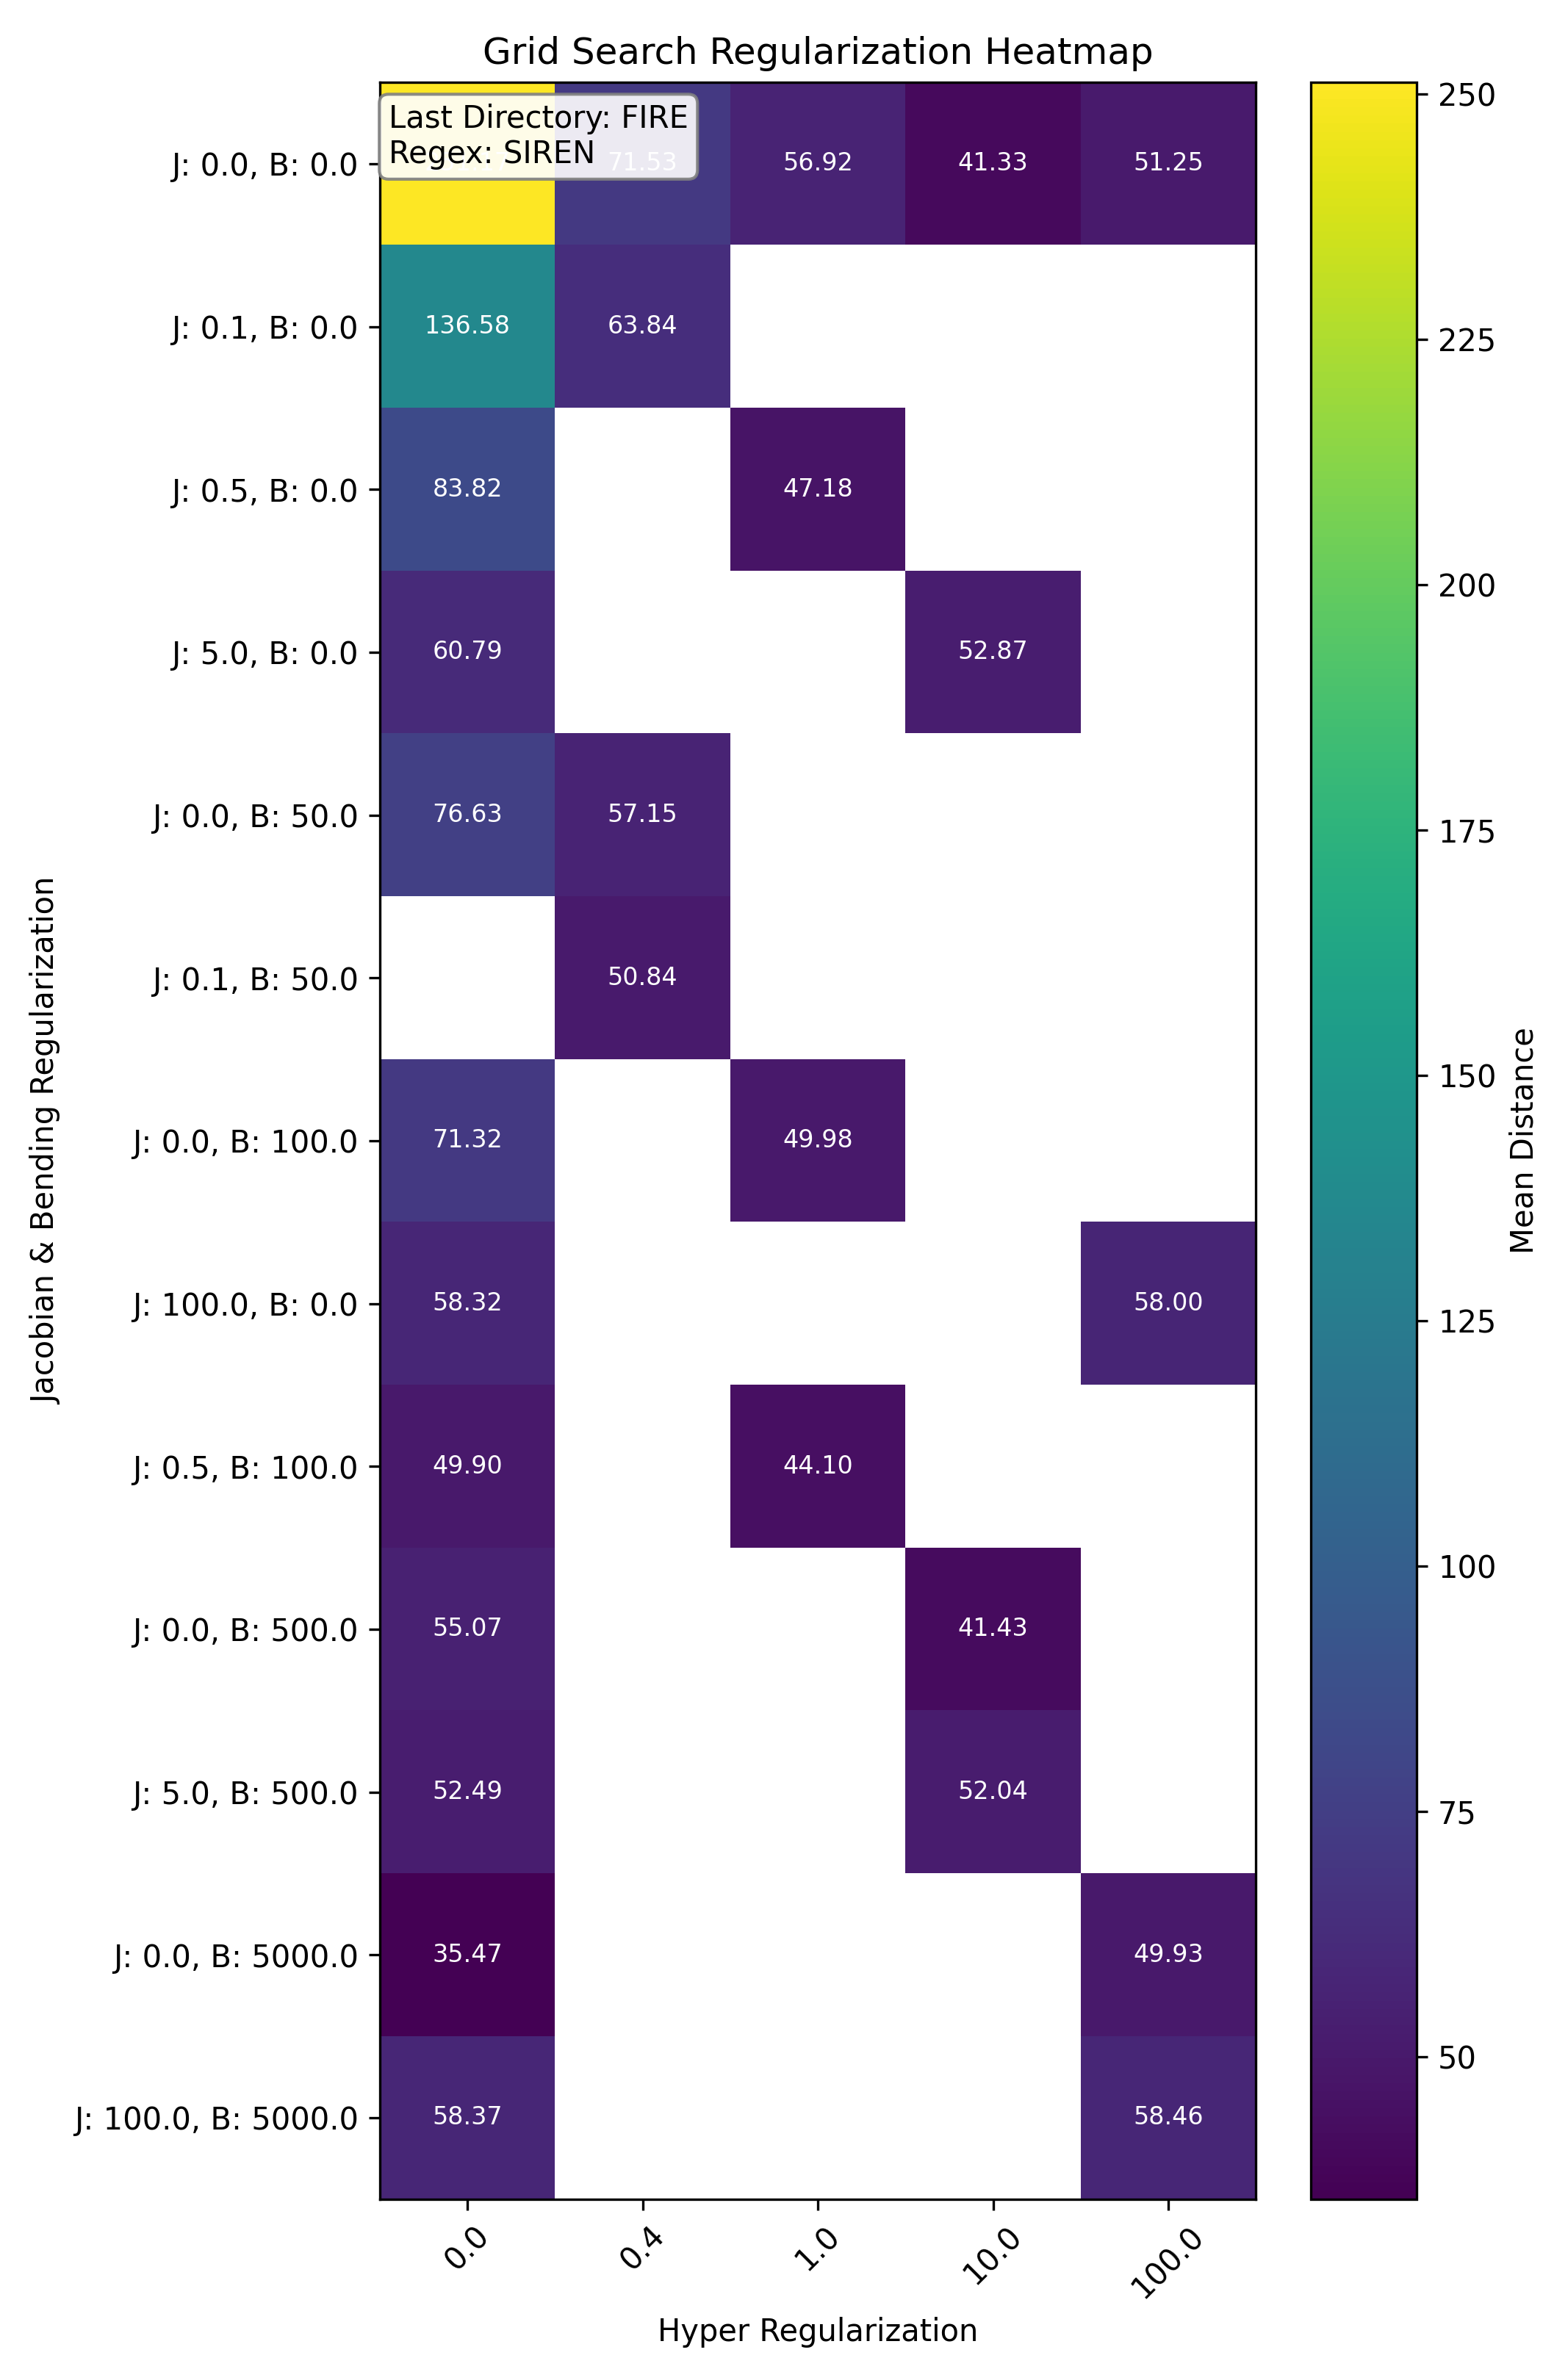
\includegraphics[width=\textwidth]{imaxes/grid_search_single_heatmap_FIRE_SIREN.png}
        \caption{FIRE - SIREN}
        \label{fig:gs_single_FIRE_SIREN}
    \end{subfigure}
    
    \vskip0\baselineskip
    
    \begin{subfigure}[b]{0.4\textwidth}
        \centering
        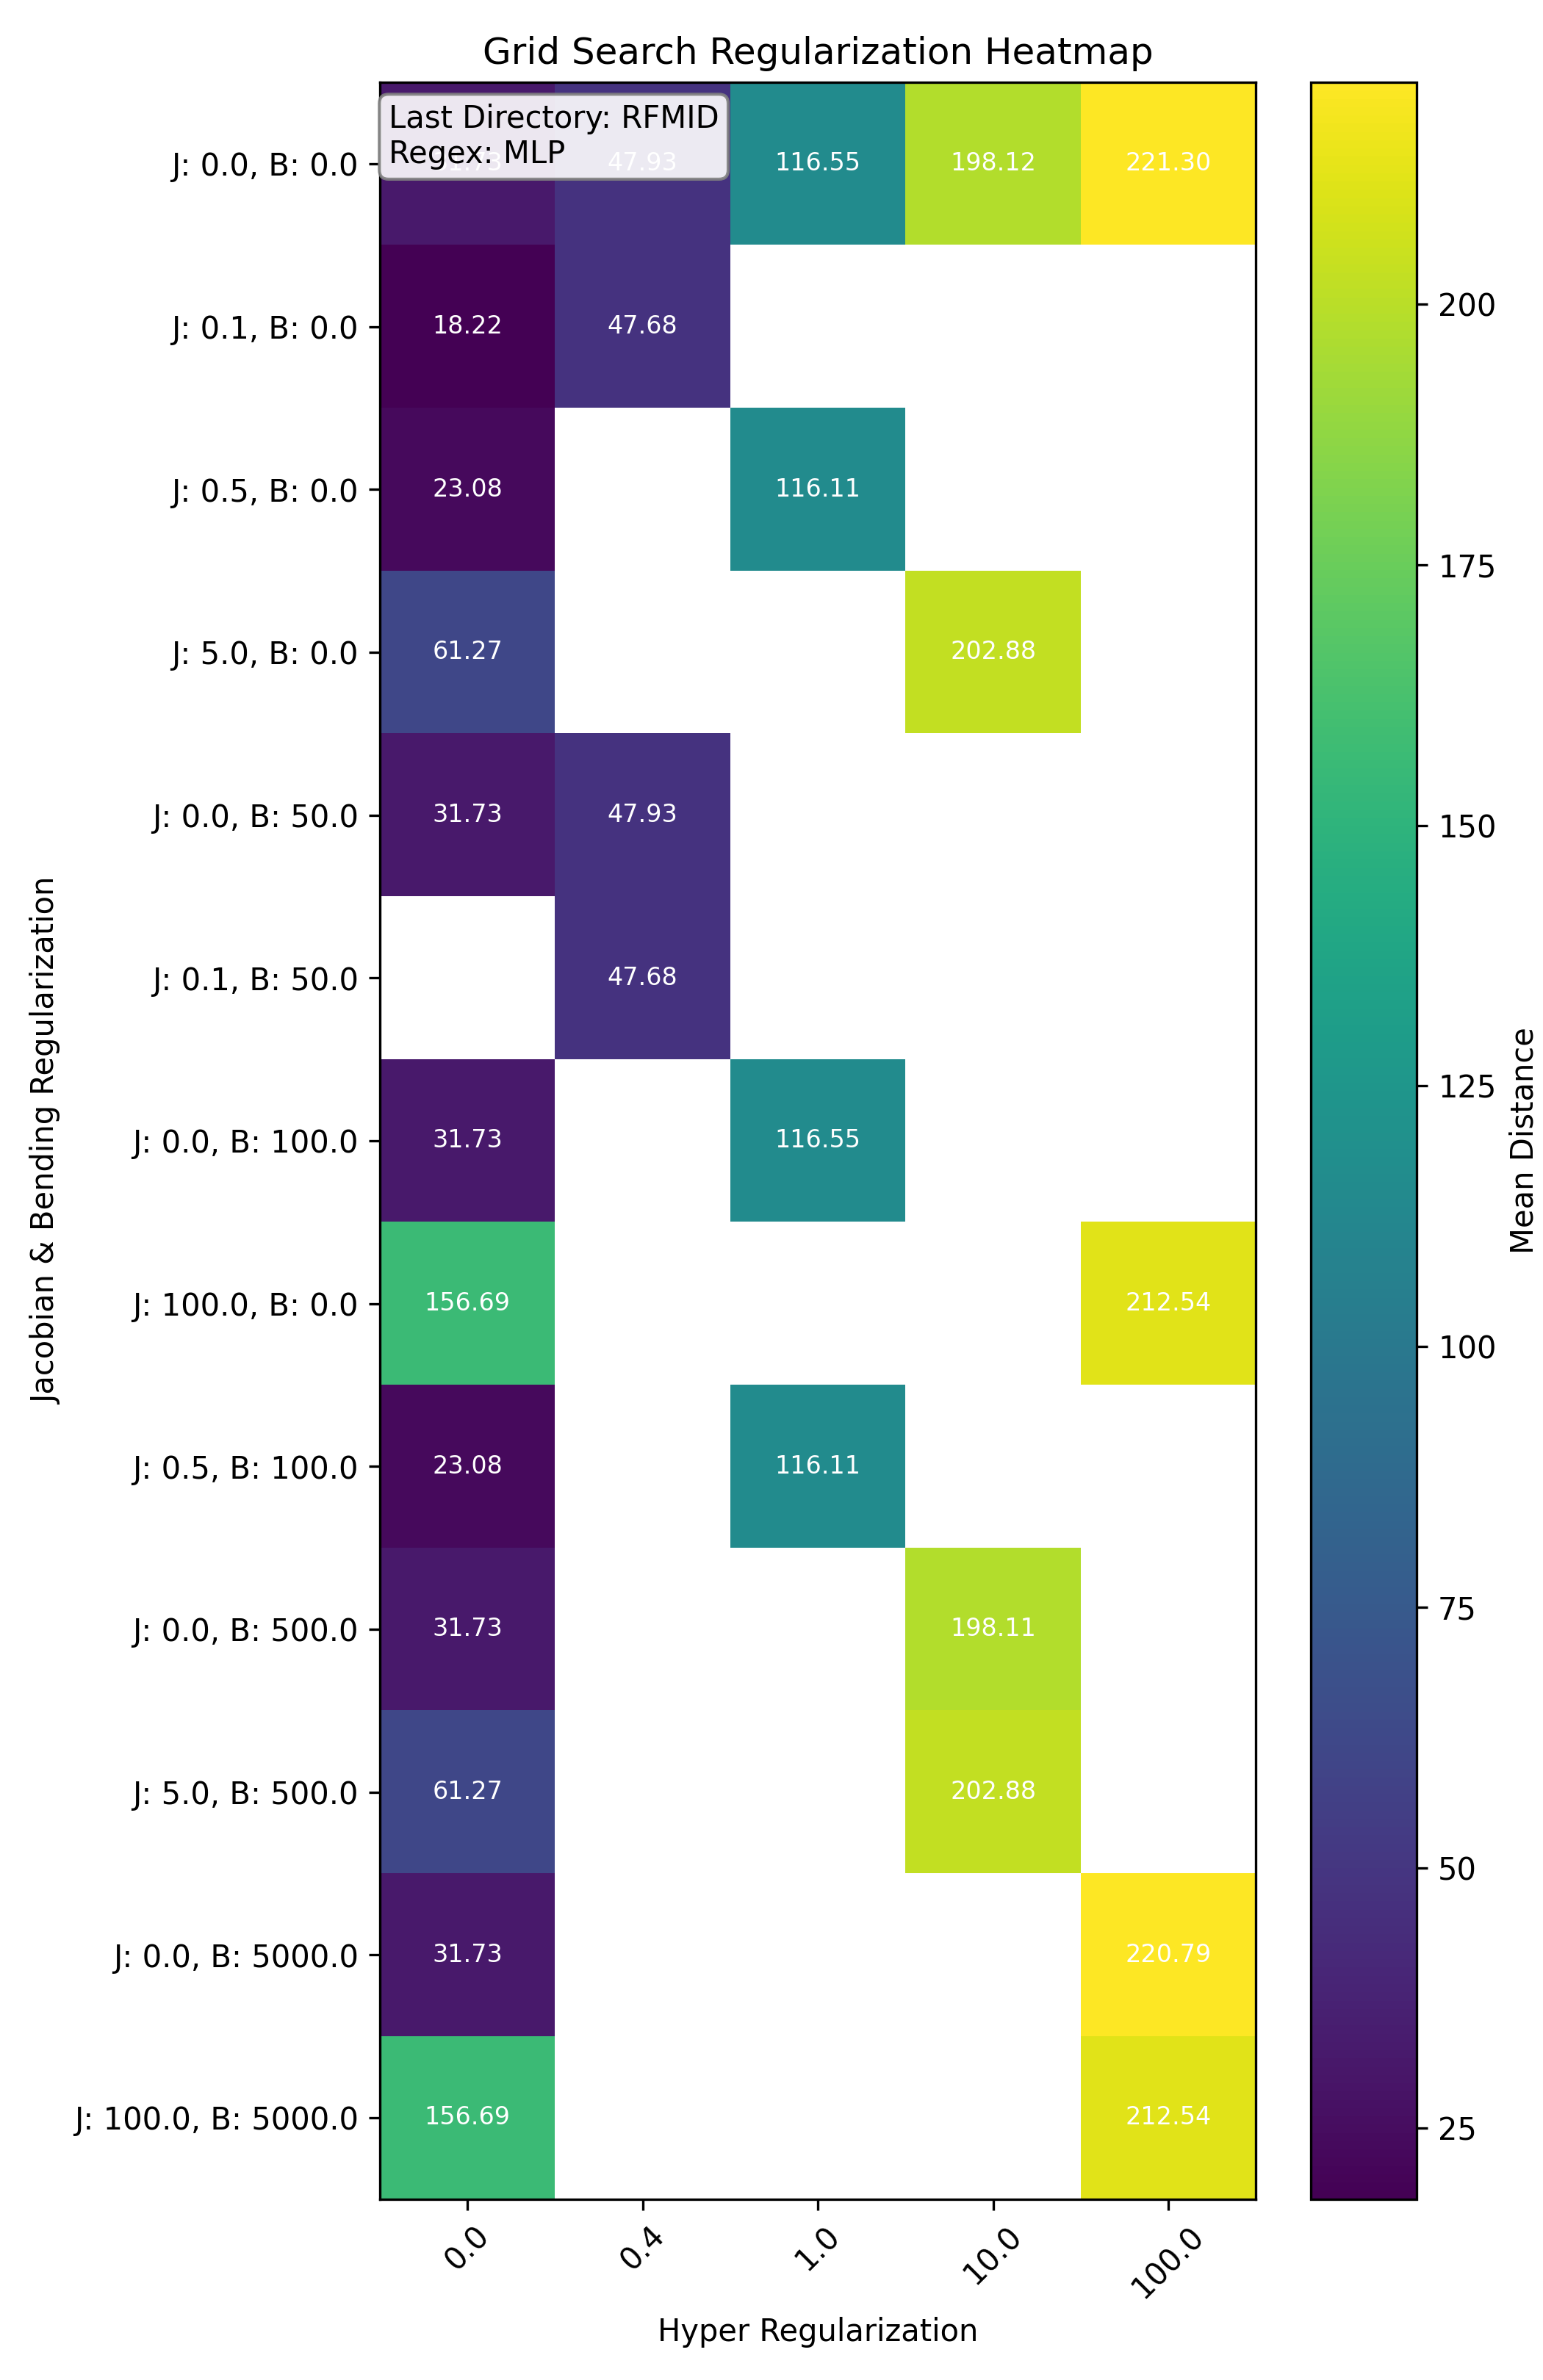
\includegraphics[width=\textwidth]{imaxes/grid_search_single_heatmap_RFMID_MLP.png}
        \caption{RFMID - Relu}
        \label{fig:gs_single_RFMID_MLP}
    \end{subfigure}\hfill
    \begin{subfigure}[b]{0.4\textwidth}
        \centering
        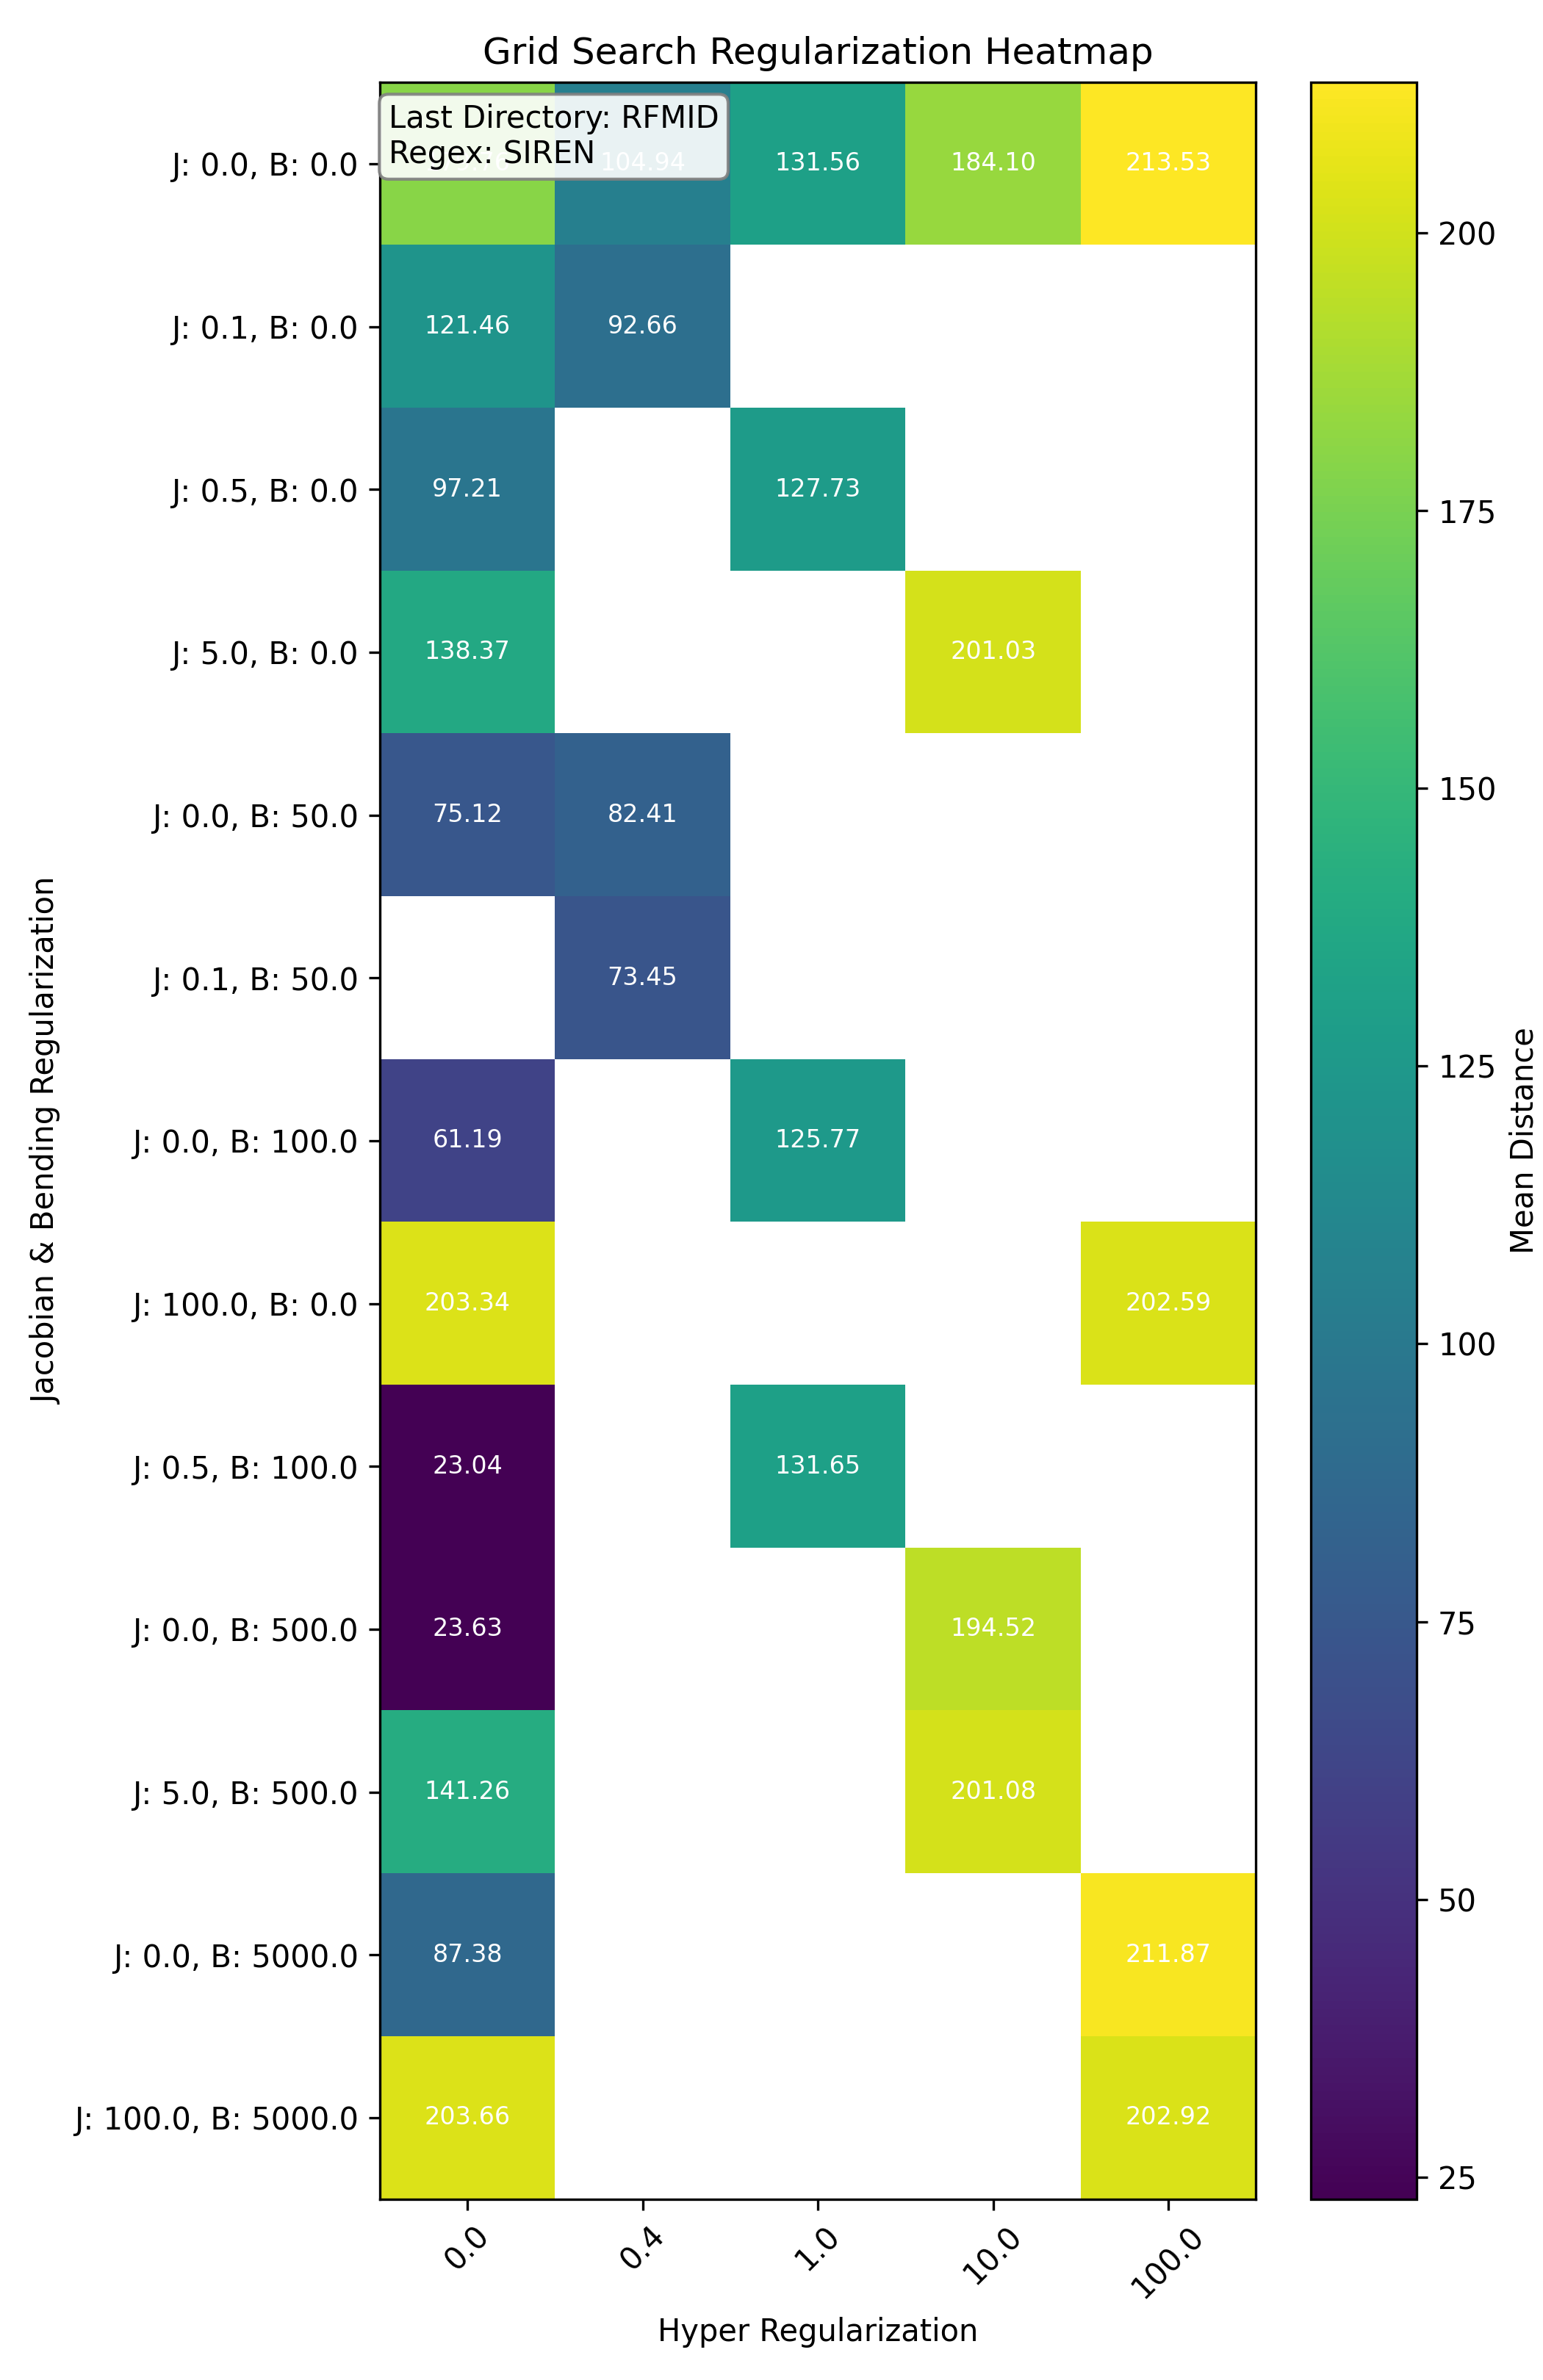
\includegraphics[width=\textwidth]{imaxes/grid_search_single_heatmap_RFMID_SIREN.png}
        \caption{RFMID - SIREN}
        \label{fig:gs_single_RFMID_SIREN}
    \end{subfigure}
    
    \caption{Mapa de calor cos resultados de diferentes combinacións de termos de regularización e funcións de activación sobre os datasets FIRE e RFMID}
    \label{fig:gs_single_heatmaps}
\end{figure}

\paragraph{Discusión}
\label{par:Discusion-reg2}

Os resultados amosan que as interaccións entre os diferentes termos de regularización e as funcións de activación son complexas e moi dependentes da parella de imaxes concreta a rexistrar.

\FloatBarrier
 \chapter{Material adicional}
\label{chap:adicional}

\section{Anexo regularization}
\label{sec:Anexo regularization}

% \begin{table}[h]
%     \centering
%     \begin{minipage}[t]{0.45\linewidth}
%         \centering
%         \scriptsize
%         \setlength{\tabcolsep}{25pt}
%         \begin{tabular}{|c|c|}
%         \hline
%         Resolution & Mean Distance \\ \hline
%         100 & 254.22 \\ \hline
%         250 & 251.29 \\ \hline
%         750 & 250.62 \\ \hline
%         1250 & 250.59 \\ \hline
%         1708 & 249.72 \\ \hline
%         \end{tabular}
%         \caption{Distancias medias para o dataset FIRE ca función de activación Relu}
%         \label{tab:mlp_mean_distances_fire}
%     \end{minipage}
%     \hfill
%     \begin{minipage}[t]{0.45\linewidth}
%         \centering
%         \scriptsize
%         \setlength{\tabcolsep}{25pt}
%         \begin{tabular}{|c|c|}
%         \hline
%         Resolution & Mean Distance \\ \hline
%         100 & 266.43 \\ \hline
%         250 & 263.85 \\ \hline
%         750 & 263.19 \\ \hline
%         1250 & 258.56 \\ \hline
%         1708 & 258.06 \\ \hline
%         \end{tabular}
%         \caption{Distancias medias para o dataset FIRE ca función de activación SIREN}
%         \label{tab:siren_mean_distances_fire}
%     \end{minipage}
% \end{table}

% \begin{table}[h]
%     \centering
%     \begin{minipage}[t]{0.45\linewidth}
%         \centering
%         \scriptsize
%         \setlength{\tabcolsep}{25pt}
%         \begin{tabular}{|c|c|}
%         \hline
%         Resolution & Mean Distance \\ \hline
%         100 & 37.29 \\ \hline
%         250 & 36.18 \\ \hline
%         750 & 36.01 \\ \hline
%         1250 & 35.03 \\ \hline
%         1708 & 35.04 \\ \hline
%         \end{tabular}
%         \caption{Distancias medias para o dataset RFMID ca función de activación Relu}
%         \label{tab:mlp_mean_distances_rfmid}
%     \end{minipage}
%     \hfill
%     \begin{minipage}[t]{0.45\linewidth}
%         \centering
%         \scriptsize
%         \setlength{\tabcolsep}{25pt}
%         \begin{tabular}{|c|c|}
%         \hline
%         Resolution & Mean Distance \\ \hline
%         100 & 68.12 \\ \hline
%         250 & 73.42 \\ \hline
%         750 & 77.55 \\ \hline
%         1250 & 67.33 \\ \hline
%         1708 & 67.31 \\ \hline
%         \end{tabular}
%         \caption{Distancias medias para o dataset RMIFD ca función de activación SIREN}
%         \label{tab:siren_mean_distances_rfmid}
%     \end{minipage}
% \end{table}


\subsection{Figuras experimentos de regularización}
\label{subsec:figuras_experimentos_regularizacion}

\paragraph{Resultados}
\label{par:Resultados-reg2}

Os resultados da experimentación extendida da regularización, realizados sobre os datasets FIRE e RFMID, preséntanse nas figuras \ref{fig:gs_single_heatmaps}.

\begin{figure}[tbp]
    \centering
    \begin{subfigure}[b]{0.4\textwidth}
        \centering
        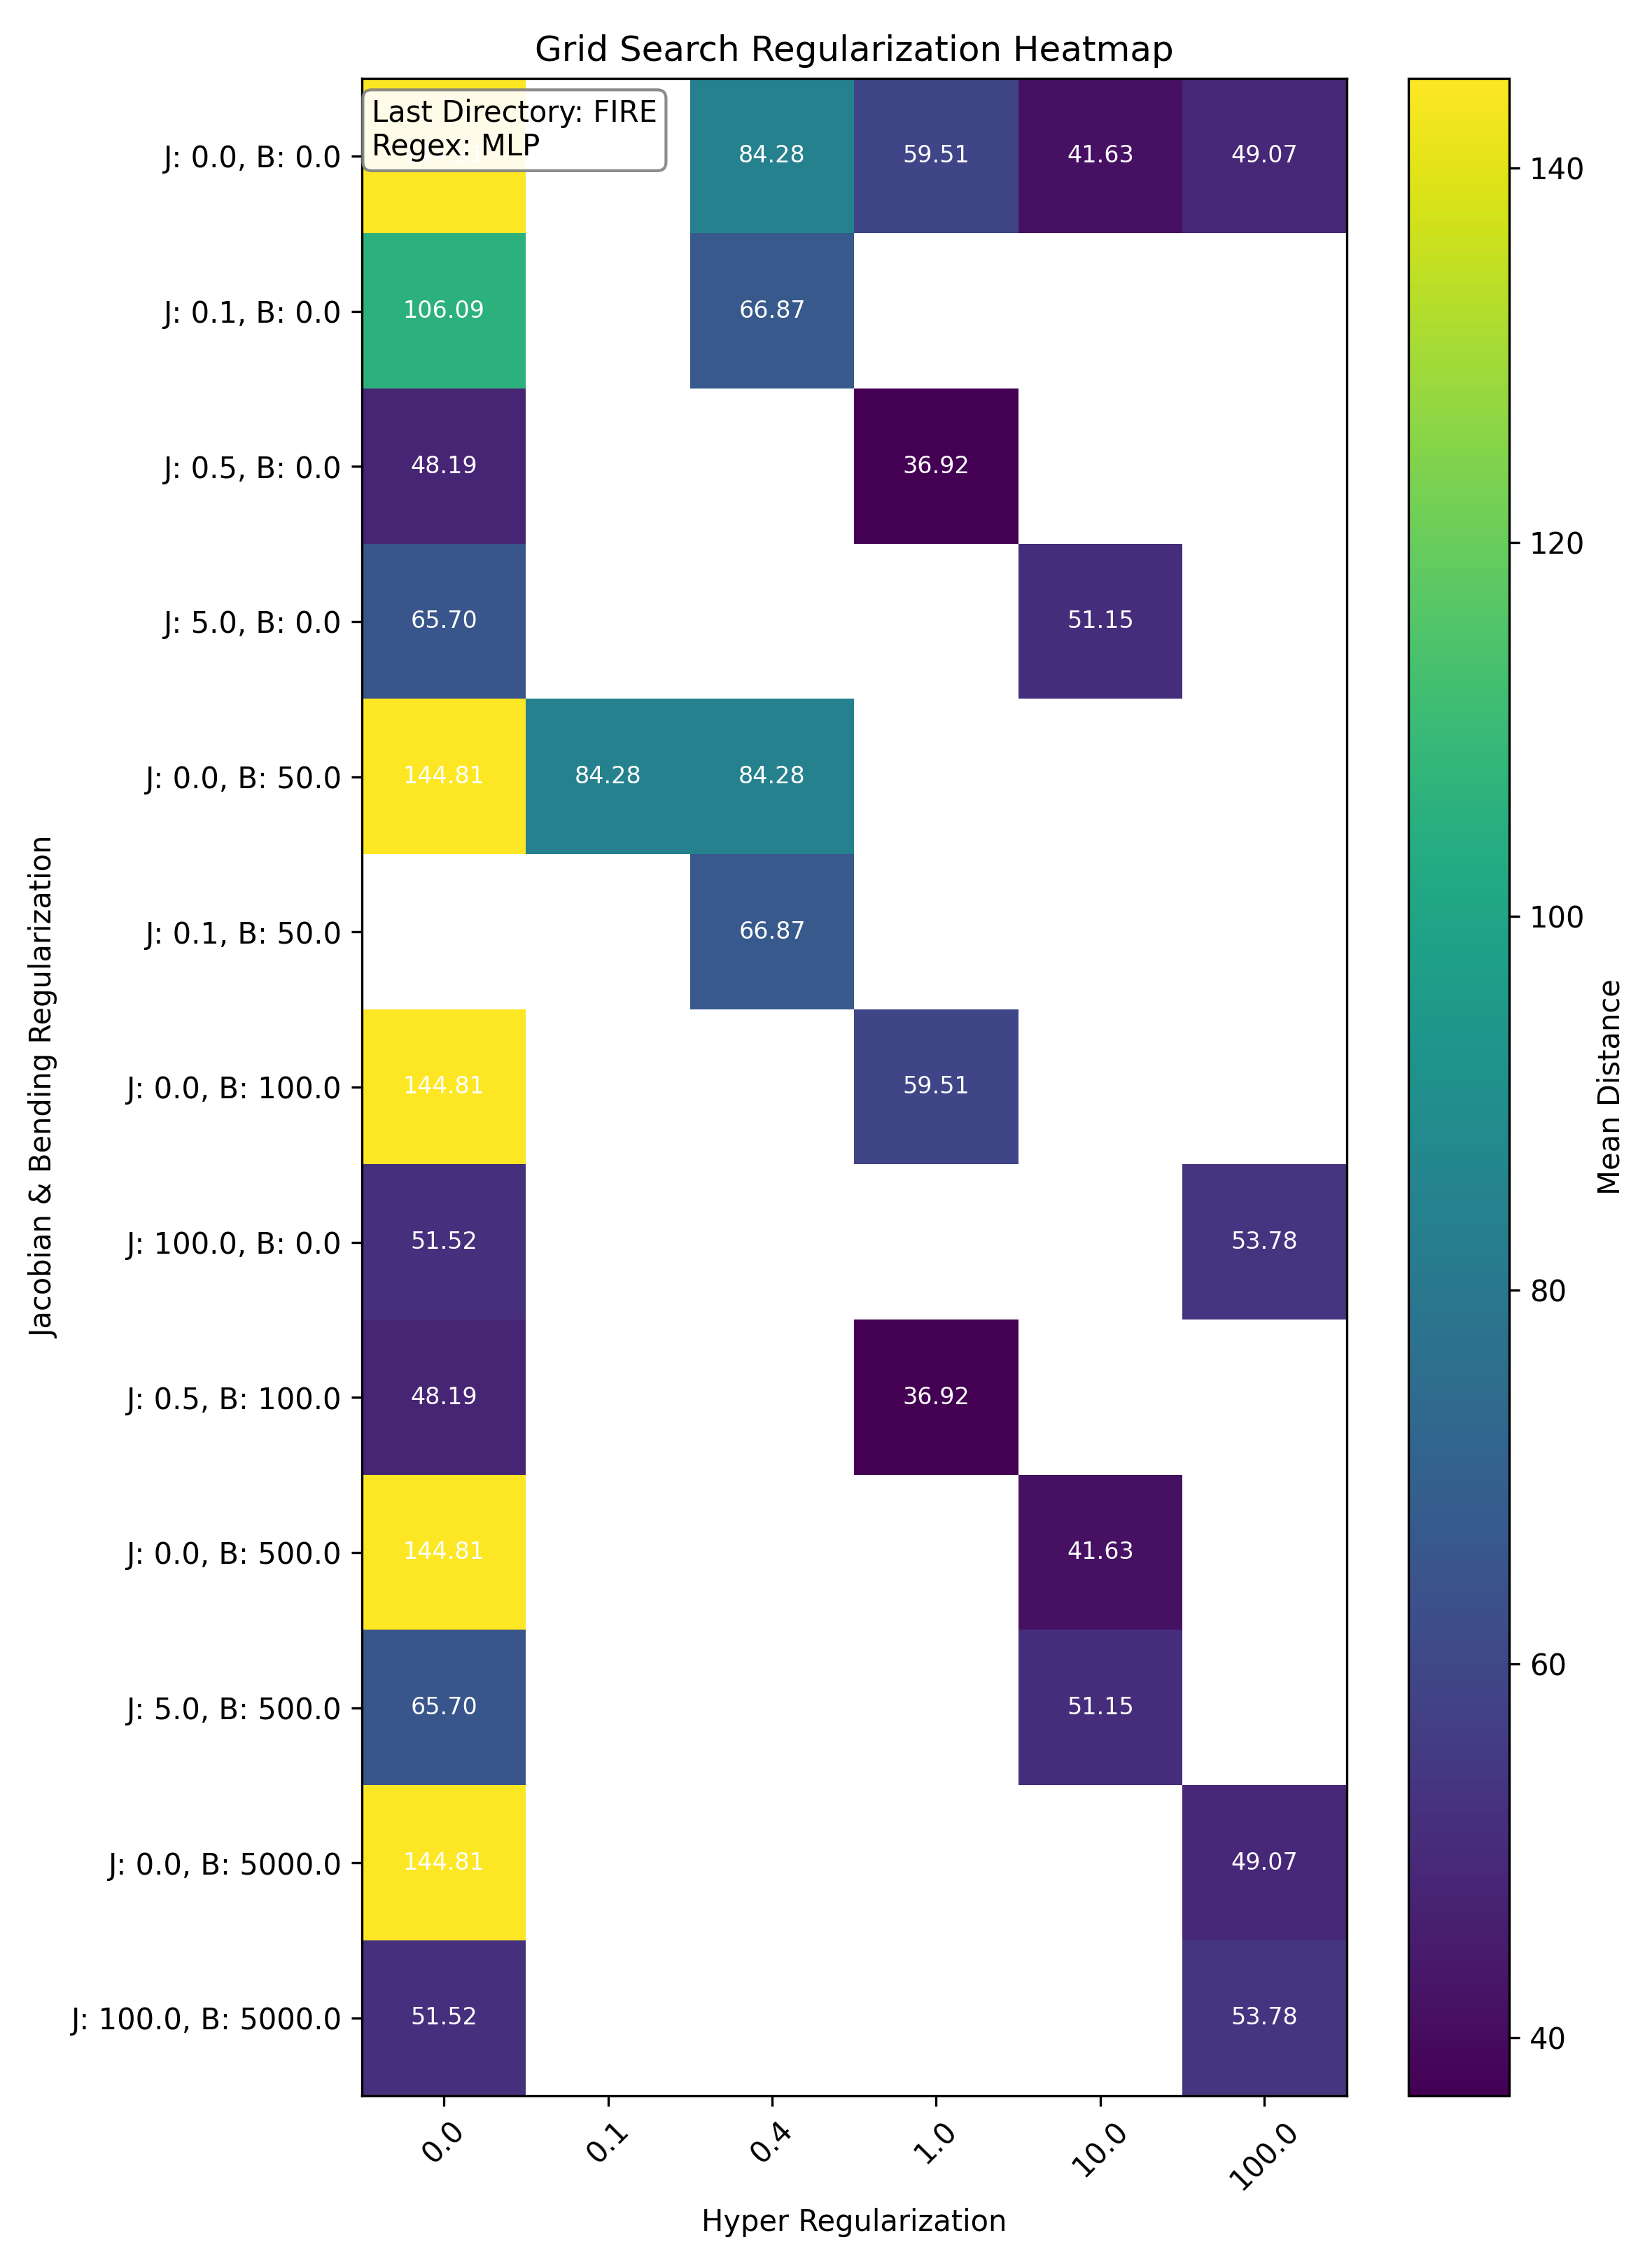
\includegraphics[width=\textwidth]{imaxes/grid_search_single_heatmap_FIRE_MLP.png}
        \caption{FIRE - Relu}
        \label{fig:gs_single_FIRE_MLP}
    \end{subfigure}\hfill
    \begin{subfigure}[b]{0.4\textwidth}
        \centering
        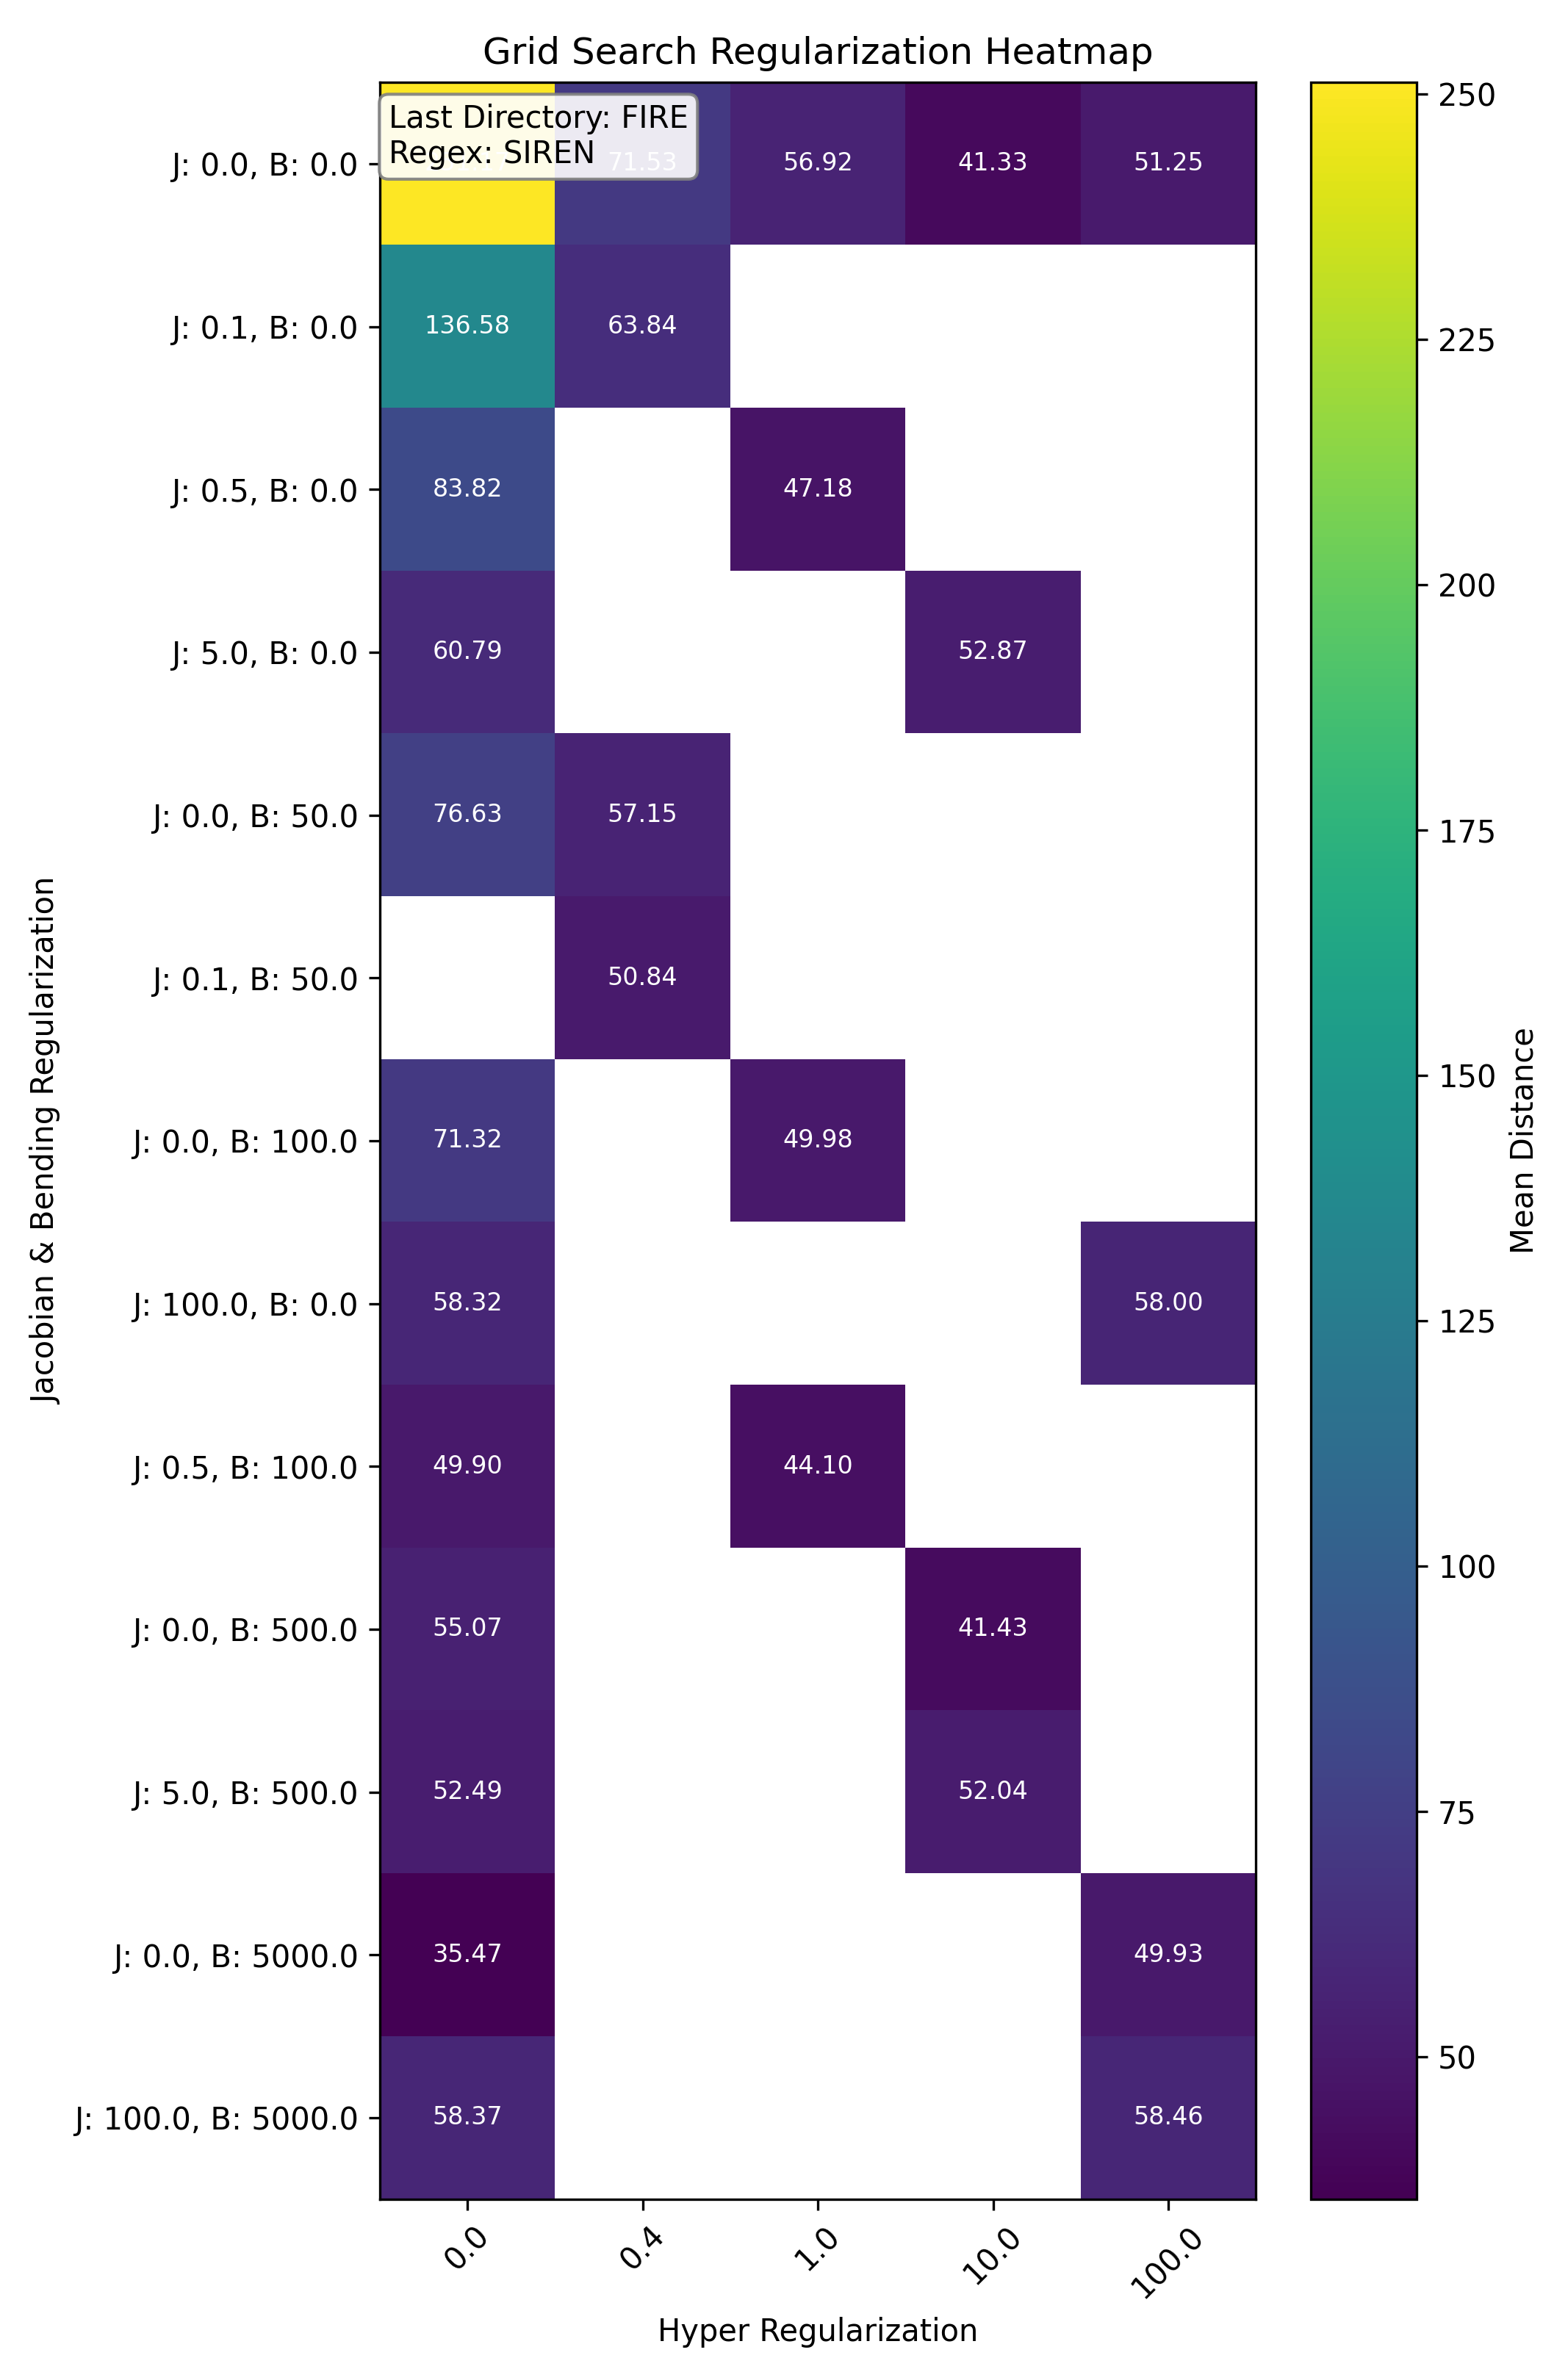
\includegraphics[width=\textwidth]{imaxes/grid_search_single_heatmap_FIRE_SIREN.png}
        \caption{FIRE - SIREN}
        \label{fig:gs_single_FIRE_SIREN}
    \end{subfigure}
    
    \vskip0\baselineskip
    
    \begin{subfigure}[b]{0.4\textwidth}
        \centering
        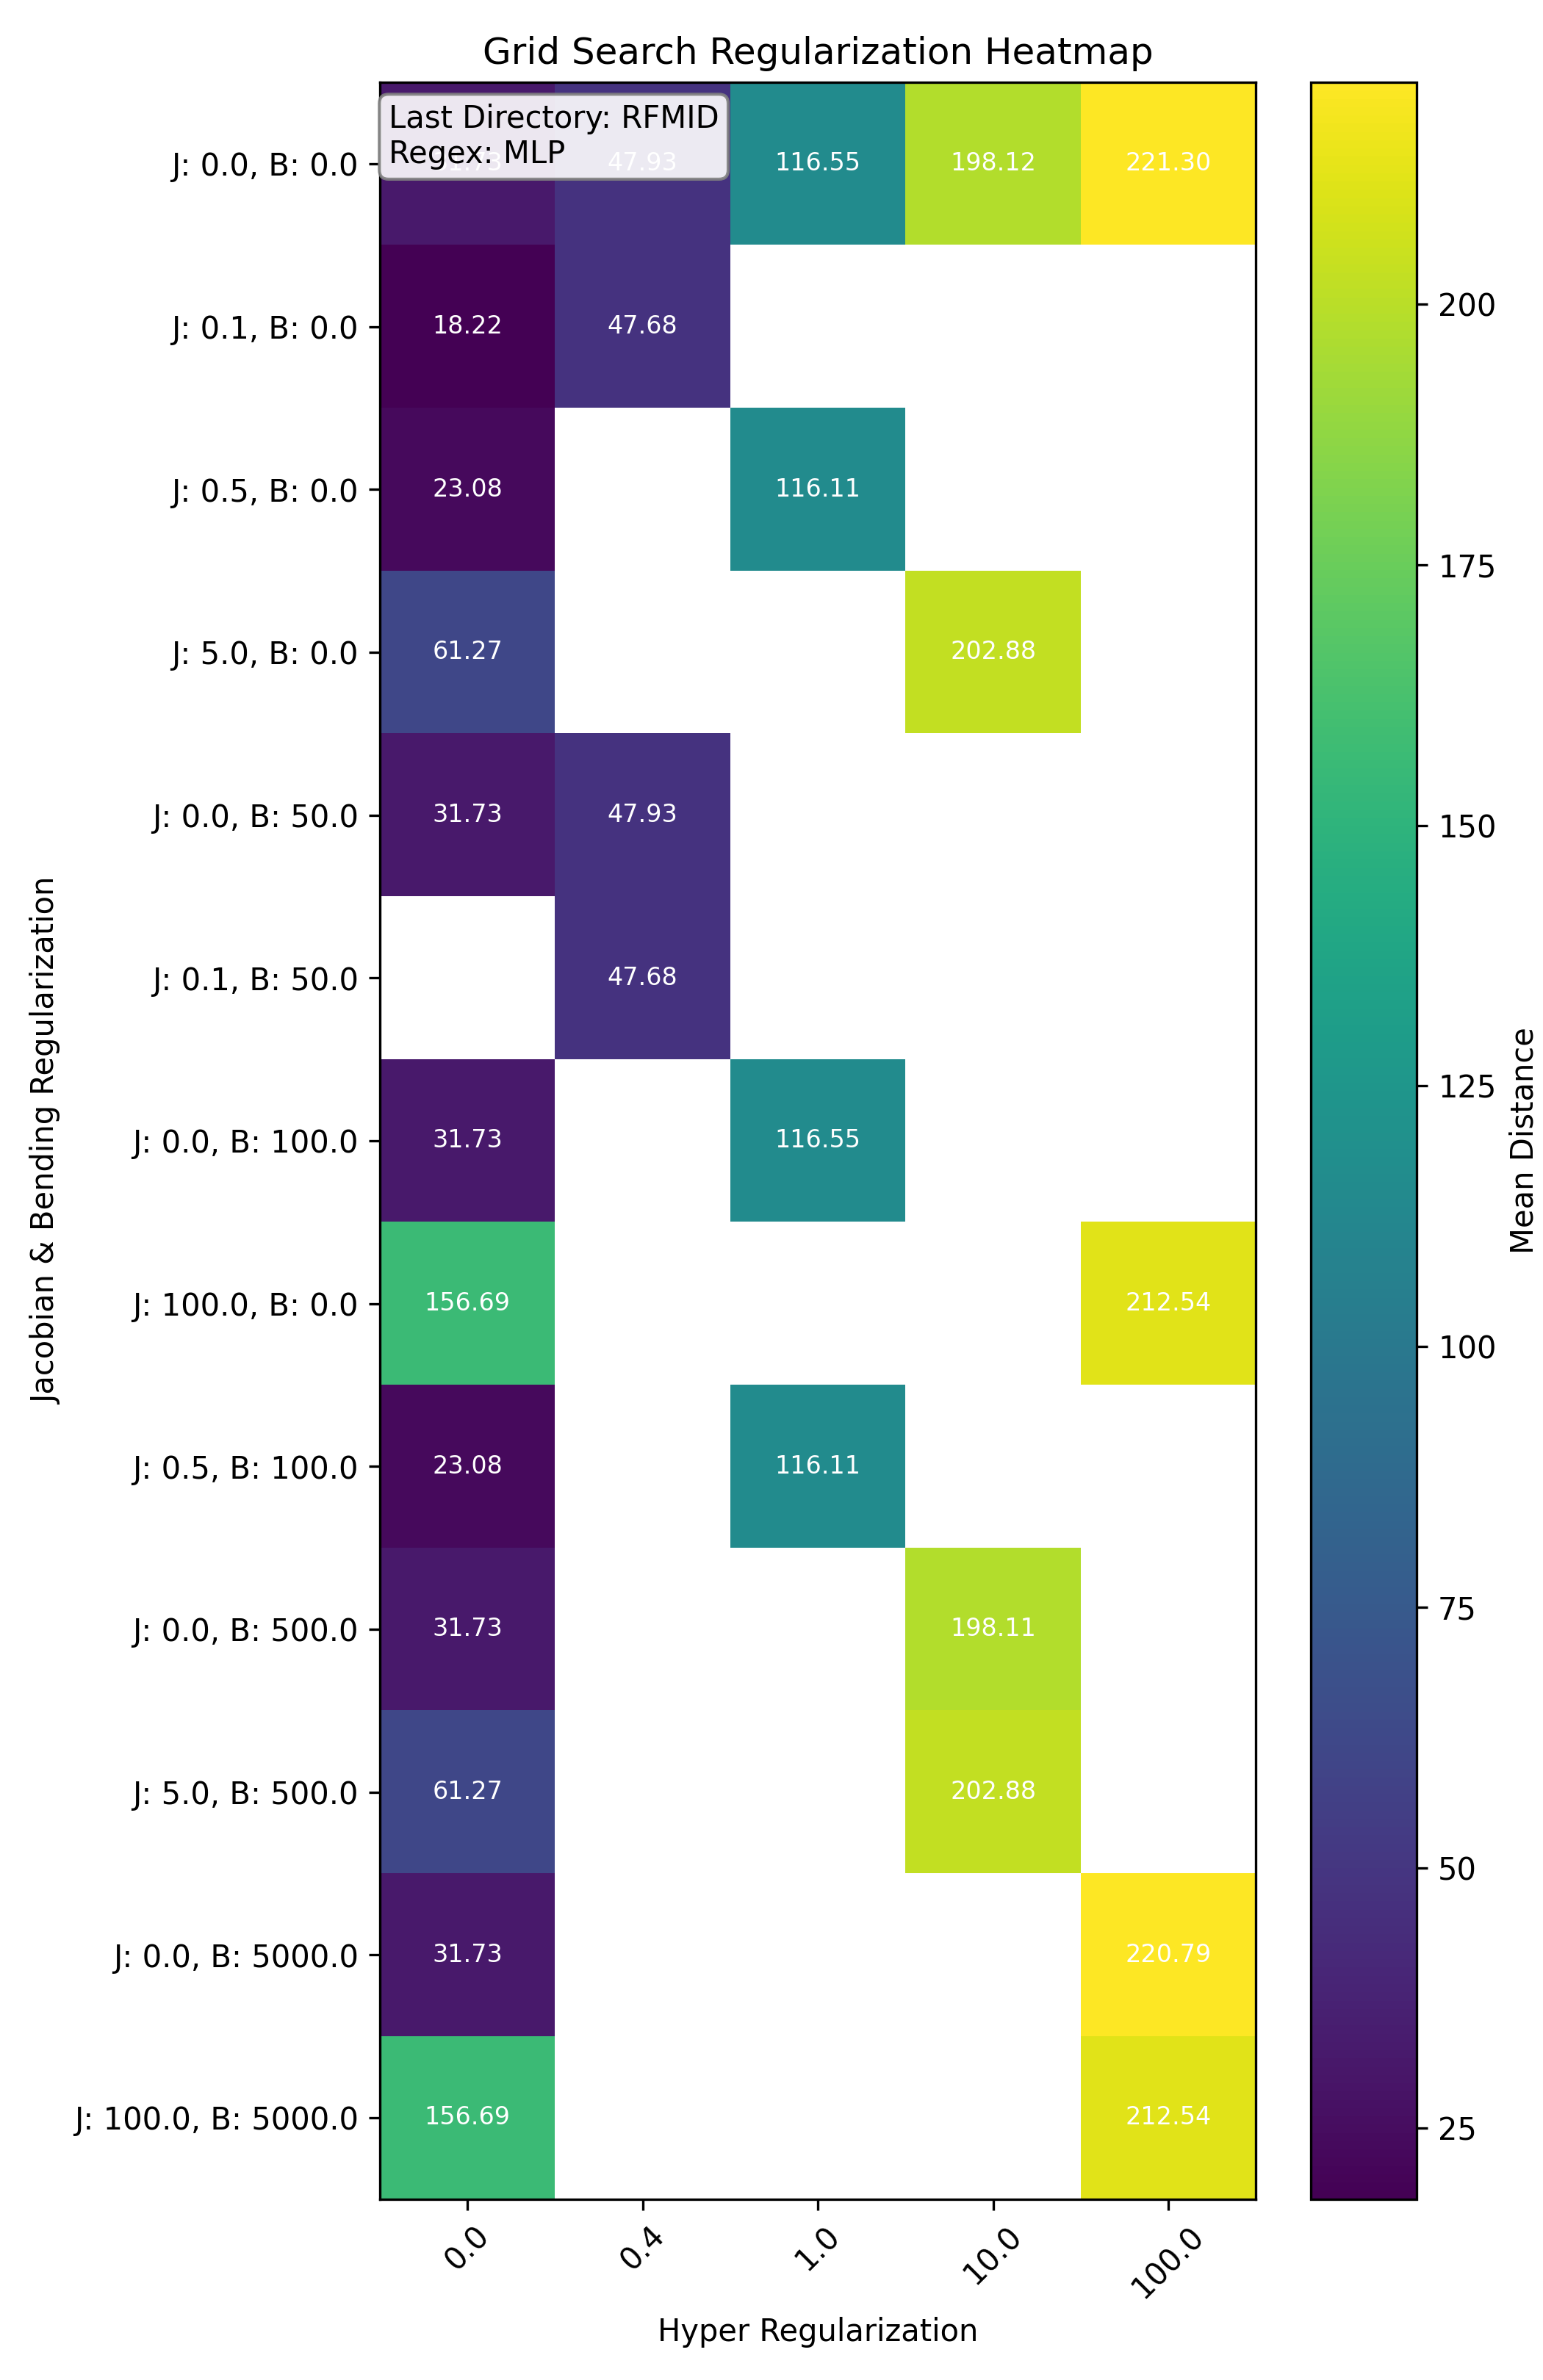
\includegraphics[width=\textwidth]{imaxes/grid_search_single_heatmap_RFMID_MLP.png}
        \caption{RFMID - Relu}
        \label{fig:gs_single_RFMID_MLP}
    \end{subfigure}\hfill
    \begin{subfigure}[b]{0.4\textwidth}
        \centering
        \includegraphics[width=\textwidth]{imaxes/grid_search_single_heatmap_RFMID_SIREN.png}
        \caption{RFMID - SIREN}
        \label{fig:gs_single_RFMID_SIREN}
    \end{subfigure}
    
    \caption{Mapa de calor cos resultados de diferentes combinacións de termos de regularización e funcións de activación sobre os datasets FIRE e RFMID}
    \label{fig:gs_single_heatmaps}
\end{figure}

\paragraph{Discusión}
\label{par:Discusion-reg2}

Os resultados amosan que as interaccións entre os diferentes termos de regularización e as funcións de activación son complexas e moi dependentes da parella de imaxes concreta a rexistrar.

\FloatBarrier

 \printglossary[type=\acronymtype,title=\nomeglosarioacronimos]
 \printglossary[title=\nomeglosariotermos]

 \bibliographystyle{IEEEtranN}
 \bibliography{\bibconfig,bibliografia/bibliografia}
 \clearpage
 
\end{document}

%%%%%%%%%%%%%%%%%%%%%%%%%%%%%%%%%%%%%%%%%%%%%%%%%%%%%%%%%%%%%%%%%%%%%%%%%%%%%%%%
